\chapter{脉搏波的预处理}
\section{引言}
本章将从PPG信号的预处理的角度对本研究过程中的相关工作进行介绍。
介绍了本研究所使用的数据来源,包括采集地点、实验方案,实验设备等。
介绍了脉搏波信号的一般处理流程。基于策略与机制分离设计理念,提出了一种新型PPG波形的初筛-复核-投票检测算法,可对较为复杂的PPG信号的精确检测。
介绍了脉搏波常见的时域描述特征,并在此基础上原创性地提出了多种新型形态学时域特征,构建了完整的脉搏波时域特征描述集合。
\section{数据采集方案设计}
为获取足量脉搏波数据,本研究于2017年6月至2019年4月期间于浙江大学附属妇产科医院进行了数据采集实验。其中,患有PE的孕妇的PPG数据做为此次实验的实验组,而正常妊娠孕妇的PPG数据则做为对照组。
数据采集实验经过浙江大学附属妇产科医院医学伦理委员会的审查并被批准进行(审查编号:20140047)。所有参与实验的孕妇均在知晓本研究目的及具体实验流程的情况下同意参与其中。
需特别引起注意的是,所有实验组孕妇均已确诊PE,出现不同程度的血压升高在内的临床症状。因此,\textbf{实验组所有患有PE的孕妇均已接受过药物治疗在内的临床干预以减轻其症状}。
\subsection{实验设备}
本研究对脉搏波数据采集仪器的专业性、可靠性都有较高要求。在考察实验场地(浙江大学附属妇产科医院麻醉科室)的诸多临床在用设备后,最后选取了美国GE公司生产的GE Healthcare CARESCAPE B650 麻醉监护仪进行数据采集。
B650监护仪可对包括12导联心电、脑电、心输出量、血氧饱和度、血压、呼出气体中$CO_{2}$与$O_{2}$成份及熵指数等专业参数进行监测,如\autoref{fig:monitor}所示。此外,B650监护仪还提供了基于血氧的表征动脉血压变化的
收缩压变化参数(Systolic pressure variation,SPV)和脉压变化参数(pulse pressure variation,PPV)\cite{GE2021,Michard1999}。
\begin{figure}[htbp]
      \centering
      \subfigure[B650监护仪及其配件]{
      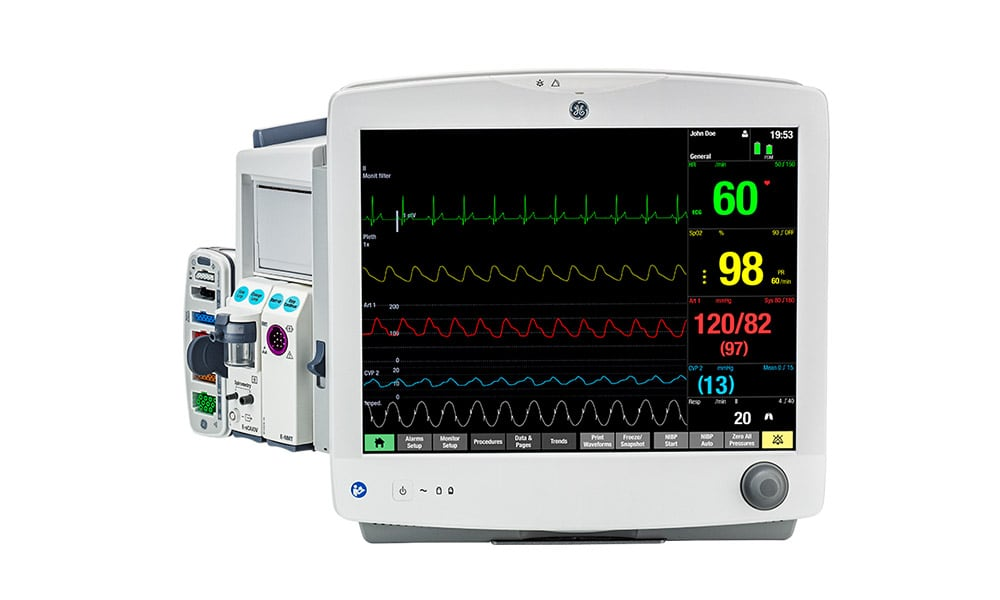
\includegraphics[width=7cm]{data_plan/monitor1}
      }
      \quad
      \subfigure[B650监护界面]{
      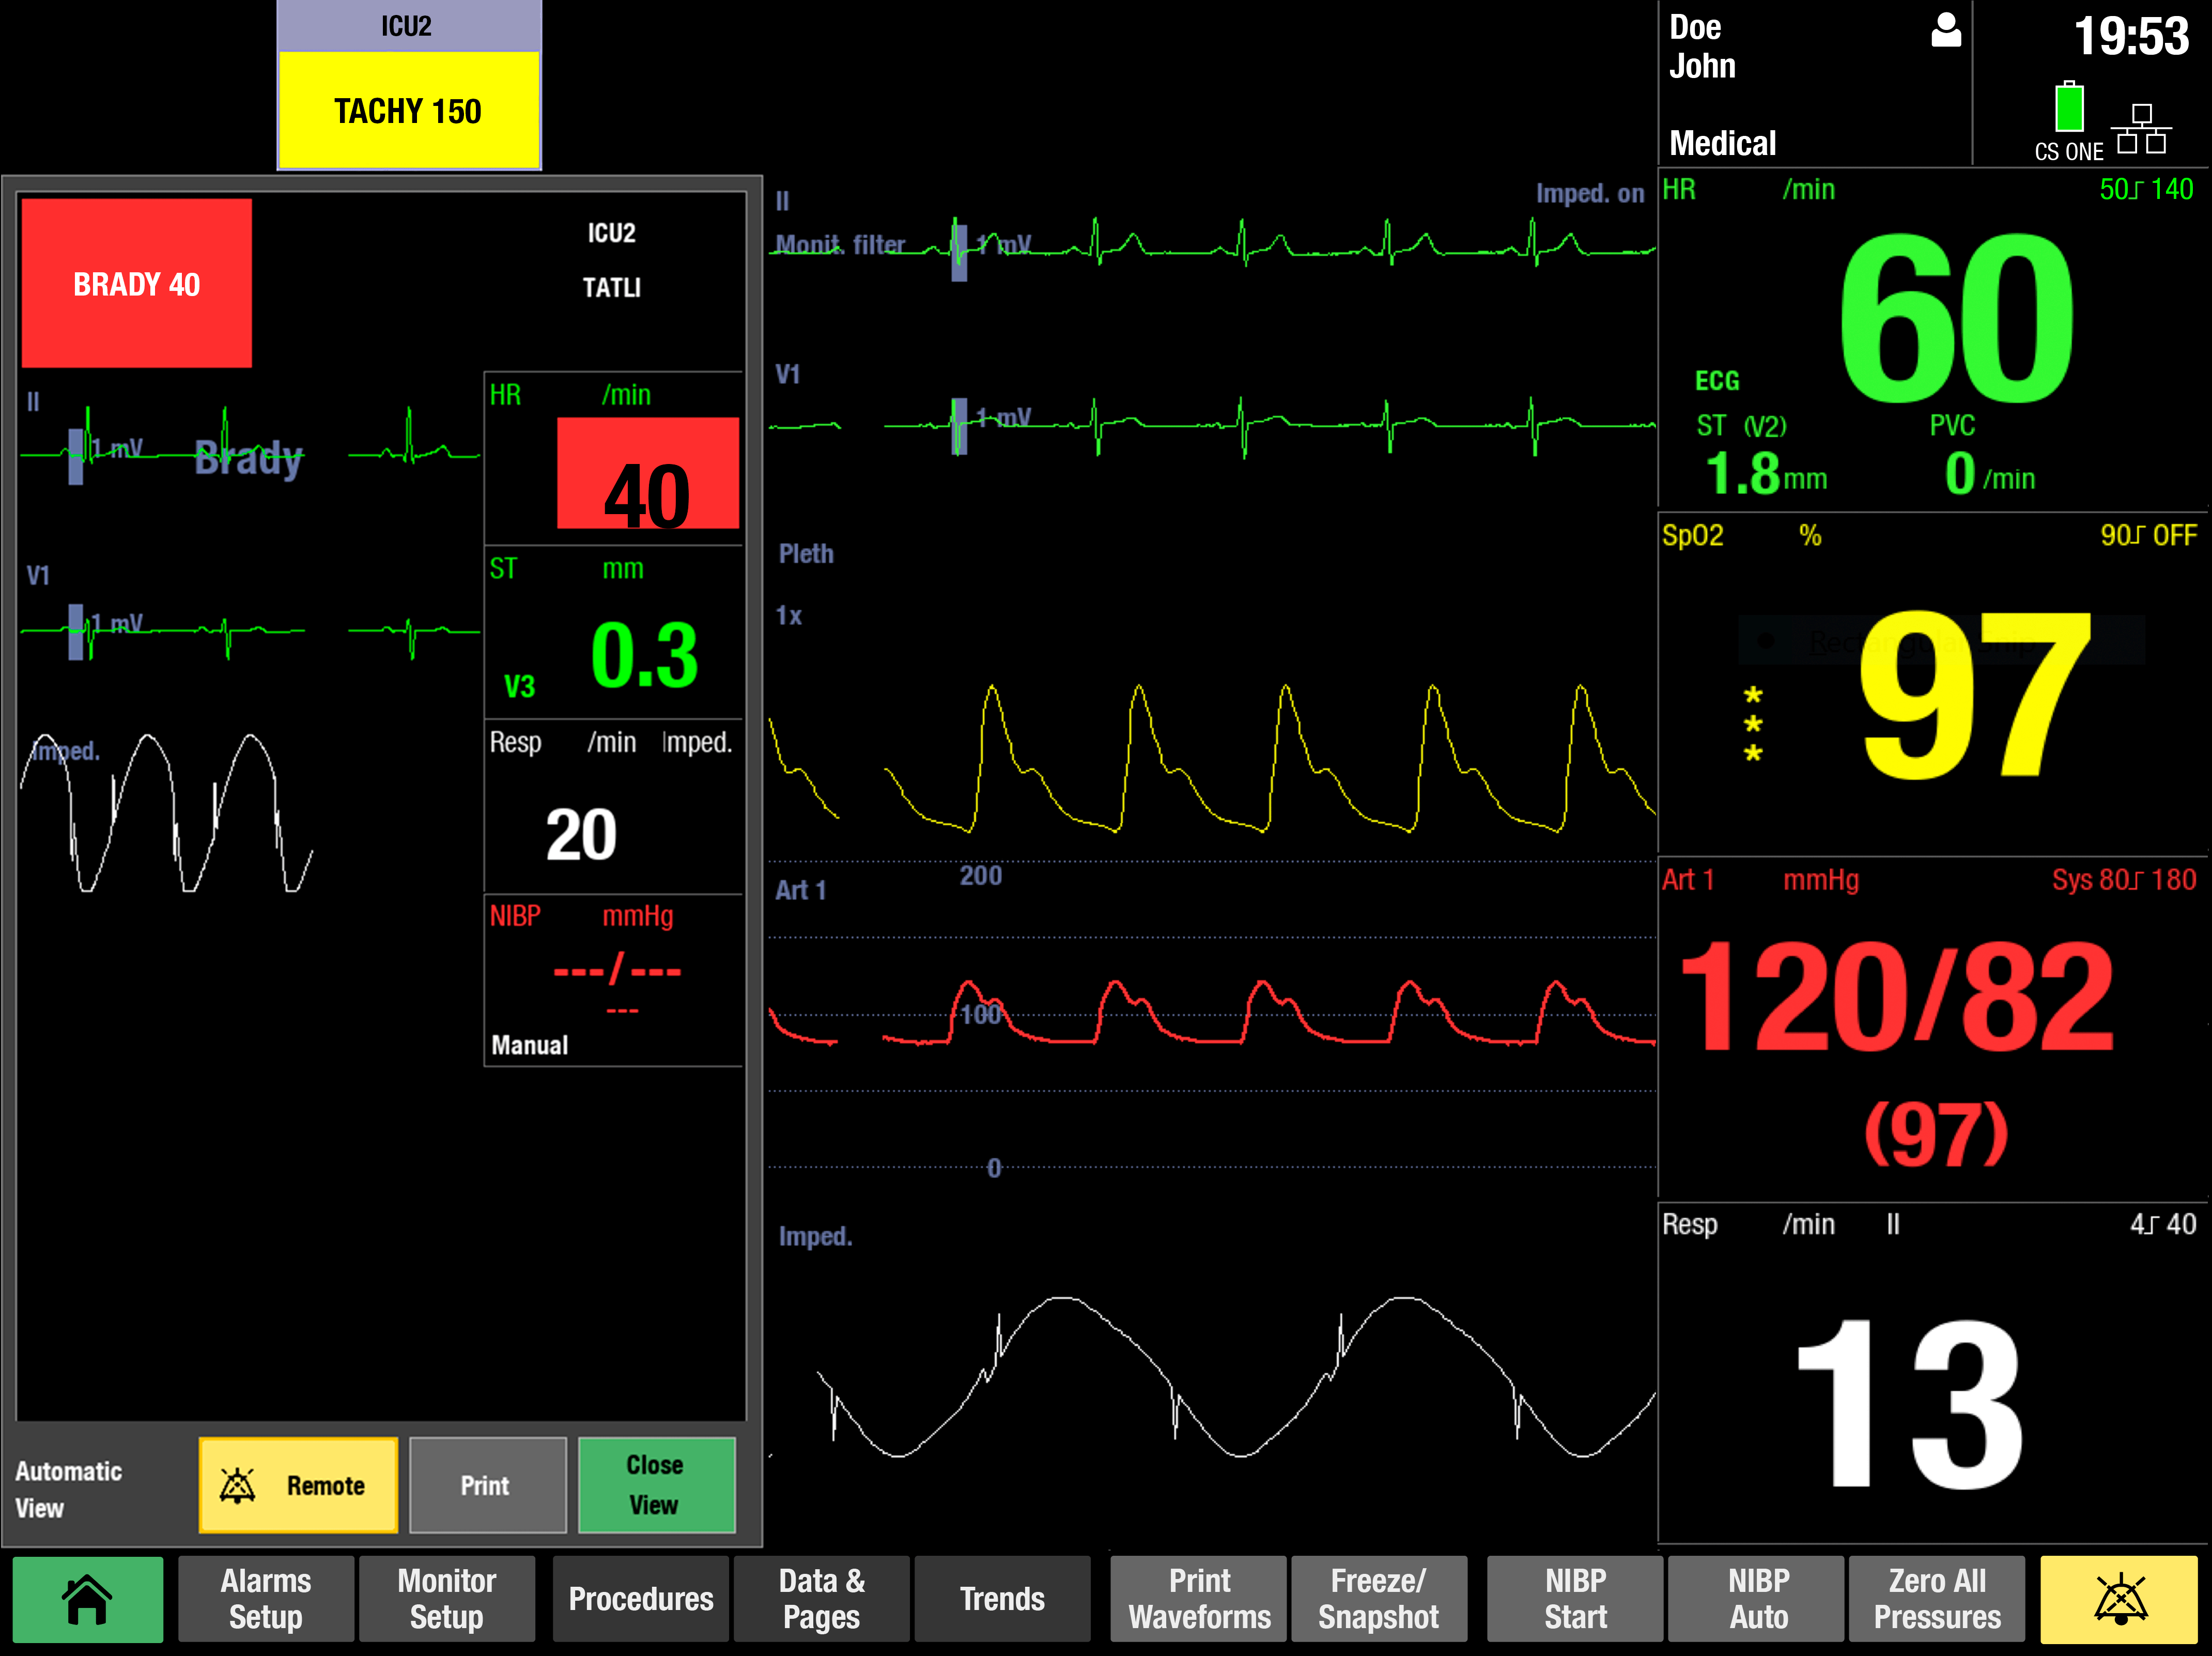
\includegraphics[width=5.5cm]{data_plan/monitor2}
      }
      \caption{\label{fig:monitor}GE Healthcare CARESCAPE B650监护仪}
\end{figure}
\subsection{实验流程}
被试人员到达数据实验采集现场后,首先实验人员会登记被试人员包括姓名、年龄、孕产史等一般信息。接着实验人员会告知被试人员本研究的研究背景与实验过程。
在征得被试人员同意后,采集人员会按前文操作规范为被试佩戴血氧采集探头\cite{Chen2021}。与血压采集过程类似\cite{FIGO},被试人员在实验全程需保持坐姿。
数据采集时选取在被试孕妇的左手食指进行使用透射式血氧探头进行采集。若被试孕妇的左手食指有损伤,则将测量部位替换为左手中指。测量时把手指放入指套内部,
指甲与传感器表面有指甲标记的部位正对,指尖触及但不超出指套顶端,确保发光管发出的所有光线全部通过被试的组织。其中,使用的血氧采集探头美国泰科公司旗下的Nellcor DS-100A型血氧传感器。 
在被试孕妇休息至少5分钟后,PPG数据开始正式记录,单次采集时长不低于1分钟。
\subsection{数据导出及复核}
由于GE公司并没有公开B650数据通讯协议,无法直接获取该设备可采集的全部生理参数的原始数据信息。通过产商技术支持提供的第三方软件,可将B650监护仪采集得到的血氧脉搏波数据以
(时间-脉搏波相对幅值)键值对的形式以CVS的文件格式导出供后续分析。其中,导出的PPG信号采样率为100$Hz$。

本研究共采集得到了80例孕妇的PPG原始数据。经复核校验,有1例正常妊娠孕妇数据因为采集时间过短、信号质量过低等原因被剔除。
最终,79例有效PPG数据进入下一阶段的分析研究,其中实验组患有PE的孕妇有效数据44例,对照组正常妊娠孕妇有效数据35例。
\section{被试孕妇人口统计学特征分析}
本小节使用了统计分析的一般方法对本研究过程中被试孕妇的多种风险因子及人口统计学特征进行了相关分析,包括被试的年龄、孕周、身高、体重、BMI指数、血压及心率等。
\subsection{变量分析方法}
在对以上风险因子展开分析之前,有必要先介绍下统计分析过程中最常用的工具与方法。

一、相关性分析

相关性分析是指对两个具备相关性的变量元素进行分析,衡量两个变量因素的相关密切程度\cite{Zhang2019}。相关性的元素之间需要存在一定的联系或者概率才可以进行相关性分析。一般可以通过散点图即可直接观察变量之间的联系,如\autoref{fig:relation}所示。
统计学上引入了相关系数$r$以量化表征变量之间的密切程度。$r$的取值范围为[-1,1],其绝对值大小反映了两变量之间相关性的强弱:当$r$>0时,表明两个变量正相关;反之,则两个变量变化趋势相反,呈负相关。

\begin{figure}[htbp]
      \centering
      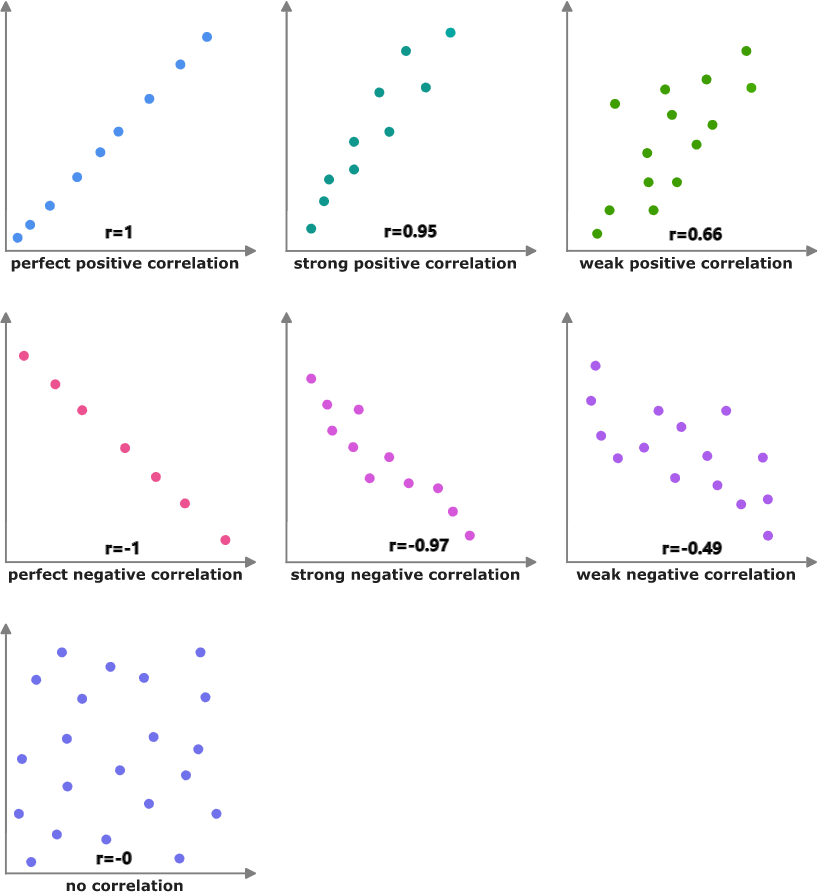
\includegraphics[width=.6\linewidth]{data_plan/relation}
      \caption[二元变量之间常见的相关关系]{\label{fig:relation}二元变量之间常见的相关关系\cite{IXL2022}}
\end{figure}

常用的相关性分析方法有皮尔逊(Pearson)相关性分析法与斯皮尔曼(Spearman)相关性分析法,利用这两种方法计算得到的相关系数也对应被称为皮尔逊相关系数$r_p$与斯皮尔曼相关系数$r_s$:
\begin{equation}
      \label{equ:spearman}
      r_s=1-\frac{6\sum_{i=1}^{n}(x_{i}-y_{i})^2}{n(n^2-1)}
\end{equation}
\begin{equation}
      \label{equ:pearson}
      r_p=\frac{\sum_{i=1}^n{(x_i- \mathop{x} \limits^-)(y_i- \mathop{y} \limits^-)}}{\sqrt{{\sum_{i=1}^n}{{(x_i- \mathop{x} \limits^-)^2\sum_{i=1}^n}{(y_i- \mathop{y} \limits^-)^2}}}}
\end{equation}

一般认为,斯皮尔曼相关性分析适用于对存在单调性关系的变量进行检测,而皮尔逊相关性分析适用于对正态分布的变量进行检测。
由于斯皮尔曼相关系数的计算对变量的分布特性要求并不严格,因而应用得也更为广泛。
如\autoref{equ:spearman}所示,为计算斯皮尔曼相关系数,需要对长度为$n$的待检二元变量$X$与$Y$按升序排列,得到原始数据在排序后的序次$x$、$y$。特别地,若出现多个数据排序相同,则用这些数据的平均序次统一表征后再进行计算。

二、参数检验与非参数检验

数据的集中趋势、离散程度与分布形态是对一组数据进行描述时最常用的三个角度\cite{Hu2021}。而参数检验(parametric test)通常都是在假设数据总体服从正态分布、样本统计量服从T分布的前提下,对总体分布中的总体均值、方差及样本差等未知参数做出统计推断。
而面对总体分布类型未知或分布类型已知,但不对称或变量无法精准测量的数据,或样本容量小、无法运用中心极限定理进行相关参数检验时,
另一类不以特定的总体分布为前提、不针对总体分布参数做任何推断的分析方法也发展起来,此类分析方法被统一称为非参数检验(nonparametric test)\cite{Guo2017,Hu2021,Zhang2019}。

一般而言,参数检验的精确度高于非参数检验,因此在条件允许的情况下,应优先采用参数检验。若由于各种原因导致参数检验的条件不满足,可以应用非参数检验方法对数据进行分析。
常见的非参数检验方法及其适用情形如\autoref{tab:nonparametric-test}所示。
\begin{center}
    \zihao{-4}
      \begin{longtable}{m{1.8cm}<{\centering}m{2.5cm}<{\centering}m{5cm}<{\centering}m{6cm}<{\centering}}
		\caption{常见的非参数检验方法}\\
		\label{tab:nonparametric-test}\\
		\toprule
            \textbf{样本数目}&\textbf{样本相关性}&\textbf{检验方法}&\textbf{检验方法英文名}\\
            \midrule
            \endfirsthead
            \caption[]{(续)}\\
            \toprule
            \textbf{样本数目}&\textbf{样本相关性}&\textbf{检验方法}&\textbf{检验方法英文名}\\
            \midrule
            \endhead 
            \hline
            \endfoot
            \bottomrule
            \endlastfoot
            单样本   & /     & 卡方检验  & Chi-Squared Test \\
            单样本   & /     & 二项分布检验 & Binomial Test \\
            单样本   & /     & K-S检验 & Kolmogorov–Smirnov Test \\
            单样本   & /     & 符号秩检验 & Wilcoxon Signed-Rank Test \\
            单样本   & /     & 游程检验  & Wald–Wolfowitz runs Test \\
            两样本   & 独立    & Wilcxon W等级和检验 & Mann-Whitney U Test \\
            两样本   & 独立    & 摩西极端反映差异检验 & Moses Extreme Reaction Test \\
            两样本   & 独立    & K-S检验 & Kolmogorov–Smirnov Test \\
            两样本   & 独立    & 游程检验  & Wald–Wolfowitz runs Test \\
            两样本   & 相关    & 符号检验  & Sign Test \\
            两样本   & 相关    & 符号秩检验 & Wilcoxon Signed-Rank Test \\
            两样本   & 相关    & 变化显著性检验 & McNemar's Test \\
            两样本   & 相关    & 边缘一致性检验 & Marginal Homogeneity Test \\
            多样本   & 独立    & K-W平均秩检验 & Kruskal-Wallis H Test \\
            多样本   & 独立    & 中位数检验 & Median Test \\
            多样本   & 独立    & 分组分布检验 & Jonckheere-Terpstra Test \\
            多样本   & 相关    & 双向等级方差分析 & Friedman Test \\
            多样本   & 相关    & 肯德尔和谐系数检验 & Kendall's W Test \\
            多样本   & 相关    & 二分变量检验 & Cochran's Q Test \\
      \end{longtable}
\end{center}

\begin{table}[htbp]
      \centering
      \zihao{-4}
      \caption{\label{tab:factors_res}被试孕妇风险因子统计结果}
      \begin{tabular}{cccc}
      \toprule
      \textbf{检验变量(单位)}      & \textbf{实验组(n=44)} & \textbf{对照组(n=35)} & \textbf{p值} \\
      \midrule
      年龄(years) & 32.3±3.6 & 33.8±4.6 & 0.108 \\
      孕周(weeks) & 32.7±3.8 & 34.3±4.3 & 0.053 \\
      身高(cm) & 158.1±5.0 & 160.0±3.3 & 0.089 \\
      体重(kg) & \textbf{75.7±12.9} & \textbf{67.1±8.2} & 0.002* \\
      BMI(kg/cm) & \textbf{30.2±4.5} & \textbf{26.2±3.3} & <0.001* \\
      收缩压(mmhg) & \textbf{160.1±19.5} & \textbf{111.2±9.8} & <0.001* \\
      舒张压(mmhg) & \textbf{96.1±14.5} & \textbf{66.8±10.4} & <0.001* \\
      心率(bpm) & 87.0±11.9 & 87.5±13.1 & 0.656 \\
      \bottomrule
      \end{tabular}%
\end{table}%
\subsection{分析结果}
在此前数据采集阶段得到的关于所有被试的年龄、孕周、身高、体重、BMI指数、血压及心率等风险因子之间的联系关系等不属于本研究内容,故未作任何相关性分析。而
诸多风险因子等待检参数存在样本量较小、具体分布未知等客观限制因素,故对这些变量的分析均采用了非参数检验中的Wilcxon W等级和检验,亦即Mann-Whitney U检验。
U检验的基本思想是将全部样本混合后一起求秩,然后根据两组样本的秩分情况判断是否存在差异。

被试孕妇涉及的PE风险因子的经U检验后的统计结果如\autoref{tab:factors_res}所示,所有待分析变量均以平均值±标准差的形式表征。从\autoref{tab:factors_res}不难发现,实验组与对照组的被试孕妇在年龄、孕周、身高、心率等风险因子
上均无明显统计意义上的差别(p>0.05),但在收缩压与舒张压的数值上有显著差异(p<0.001),这也与被试孕妇的PE患病状态一致,符合预期。

\section{脉搏波的预处理}
本研究采集得到的一段有代表性的数据波形如\autoref{fig:samplesignal}所示。
可以看到,数据采集实验经由GE B650监护仪采集得到的PPG信号质量较高,但仍然存在着基线偏移、PPG信号重博波特征不明显等问题。这些问题可能与实验使用的传感器种类、监护仪硬件检测电路及监护仪软件处理算法等因素有关。
除此之外,某些数据样本中存在着一定的干扰无效数据(如\autoref{fig:samplesignal}中40s-55s内数据段),在进行后续处理前必须设法对其进行剔除。

鉴于此,本小节将按照\autoref{fig:process}所示的信号分析预处理流程对相关研究工作进行介绍,阐述解决原始信号的波形准确甄别及PPG波形相关特征点定位等问题过程中的的具体算法方案及技术手段。
\begin{figure}[htbp]
    \centering
    \includegraphics[width=\linewidth]{pulse_preprocess/samplesignal}
    \caption{\label{fig:samplesignal}一名被试实采PPG信号(片段)}
\end{figure}
\begin{figure}[htbp]
    \centering
    
\includegraphics[width=\linewidth]{pulse_preprocess/process.pdf}
    \caption{\label{fig:process}信号预处理流程示意}
\end{figure}

\subsection{信号滤波}
通常而言,数字滤波是信号处理的重要手段,可以依据具体使用需求,获取原始信号中特定频段的信号成分。而在人体电生理信号分析领域,滤波更是必不可少的处理步骤,此前的诸多学者们也针对特定信号结合具体使用环境设计提出了多种不同的滤波算法。
对本研究而言,如\autoref{fig:samplesignal}所示的原始PPG信号质量高、干扰噪声较少。因此,本小节中仅使用了较为简单的滑动平均滤波器对其进行了处理。

平滑滤波器本质上是一个低通滤波器,若以$X$表示原始信号,$Y$表示滤波后信号,$N$表示其滤波阶数,则有
\begin{equation}
    \label{equ:filter}
    Y(k)=\frac{1}{N}\sum_{i=0}^{N-1}X(k+i)
\end{equation}
其截止频率(cut-off frequency)与滤波阶数$N$存在以下关系\cite{malp2011,malp2022}
\begin{equation}
    \label{equ:malpf}
    f_{co} \approx 0.443 \cdot \frac{f_s}{N}    
\end{equation}
其中,$f_s$为原始信号采样率。由此可知,当滤波器的阶数越高,值越均匀,截止频率越低,滤波效果越好。在本研究中,其阶数$N$被设置为5。
由\autoref{equ:malpf}可知此时的截止频率约为89$Hz$。经此滑动滤波前后的PPG信号对比如\autoref{fig:filter}所示。

信噪比(signal-noise rate,SNR)与均方误差(root mean square error,RMSE)是最常用的评估滤波效果的两个指标,其定义分别为
\begin{equation}
    \label{equ:snr}
    SNR=10 \cdot \log_{10}\frac{\sum_{i=1}^{n}{(X_i-\mathop{X} \limits^-})^2}{\sum_{i=1}^{n}{(X_i-Y_i})^2}
\end{equation}
\begin{equation}
    \label{equ:rmse}
    RMSE=\sqrt{\frac{\sum_{i=1}^{n}{(X_i-Y_i})^2}{n}}
\end{equation}
对\autoref{fig:filter}信号段进行检测,可得$SNR=33.19$,$RMSE=6.27$。此时,PPG信号波形特征已比较清晰,可以满足后续分析需求。
\begin{figure}[htbp]
    \centering
    \subfigure[原始PPG信号]{
    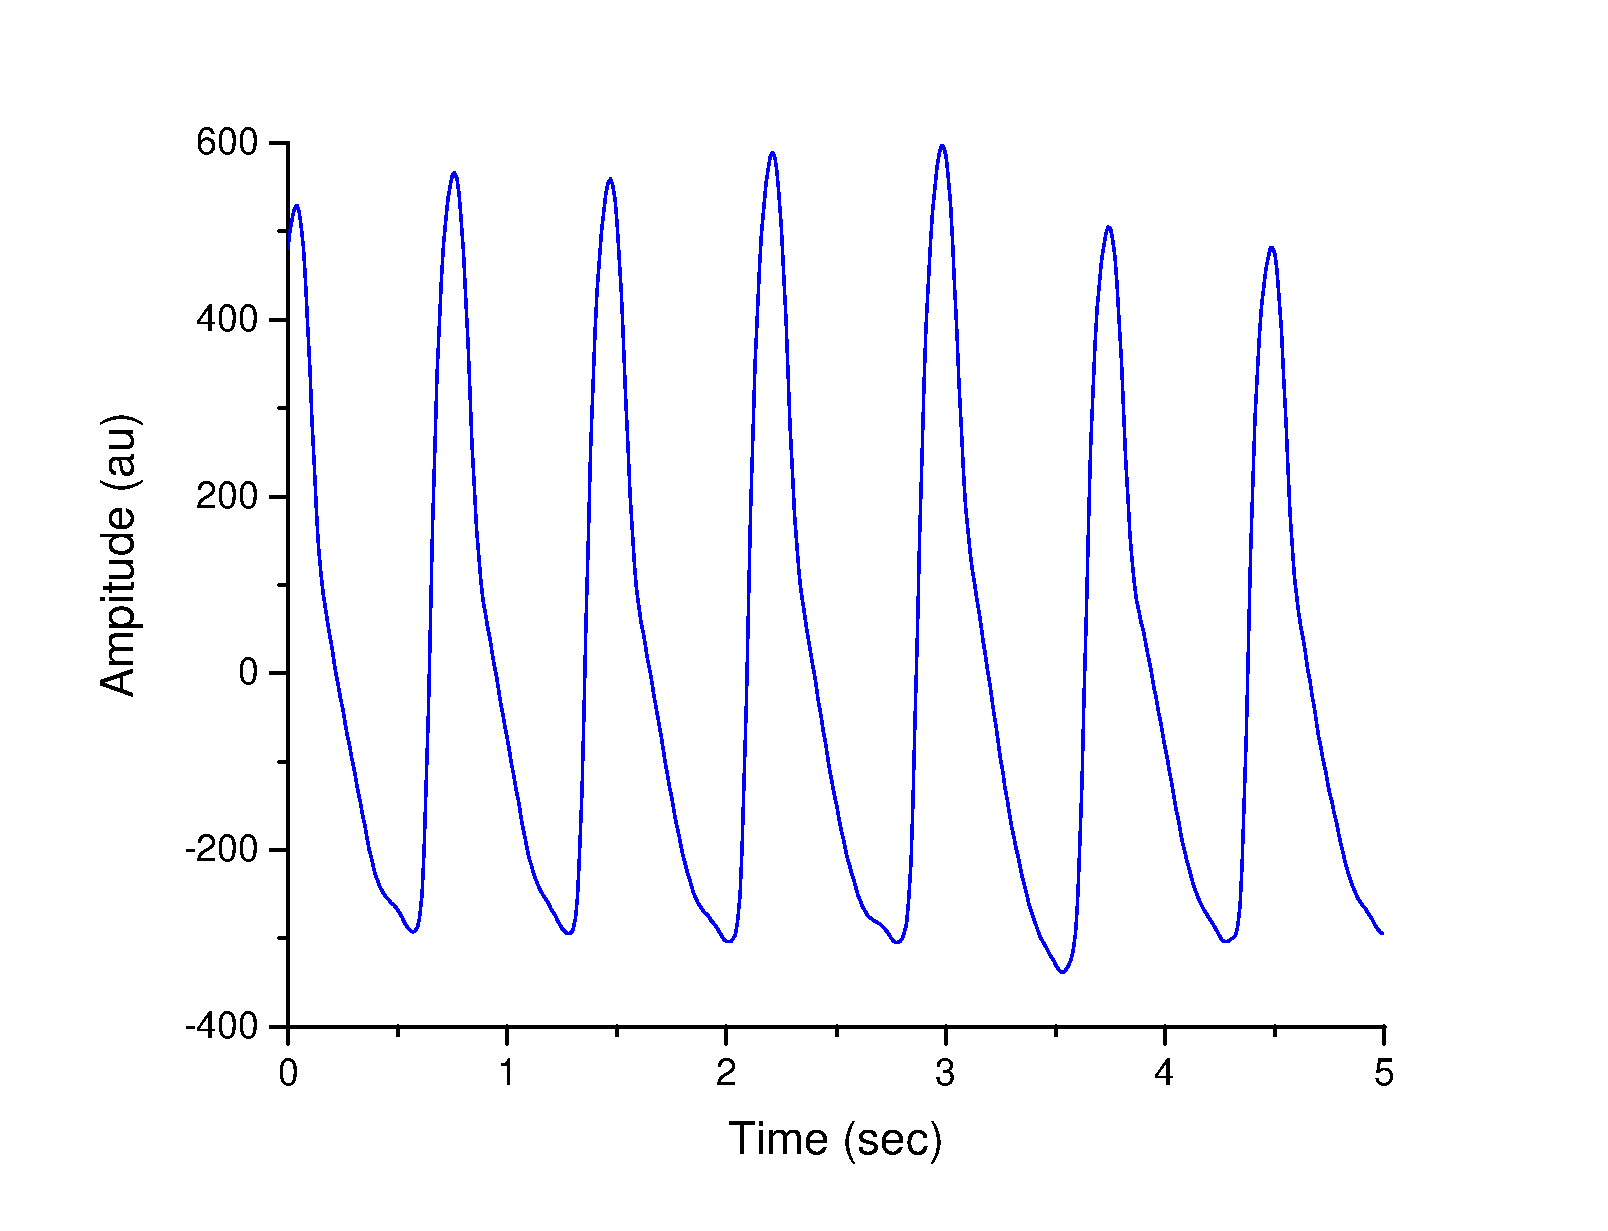
\includegraphics[width=6cm]{pulse_preprocess/before}
    }
    \quad
    \subfigure[平滑滤波后PPG信号]{
    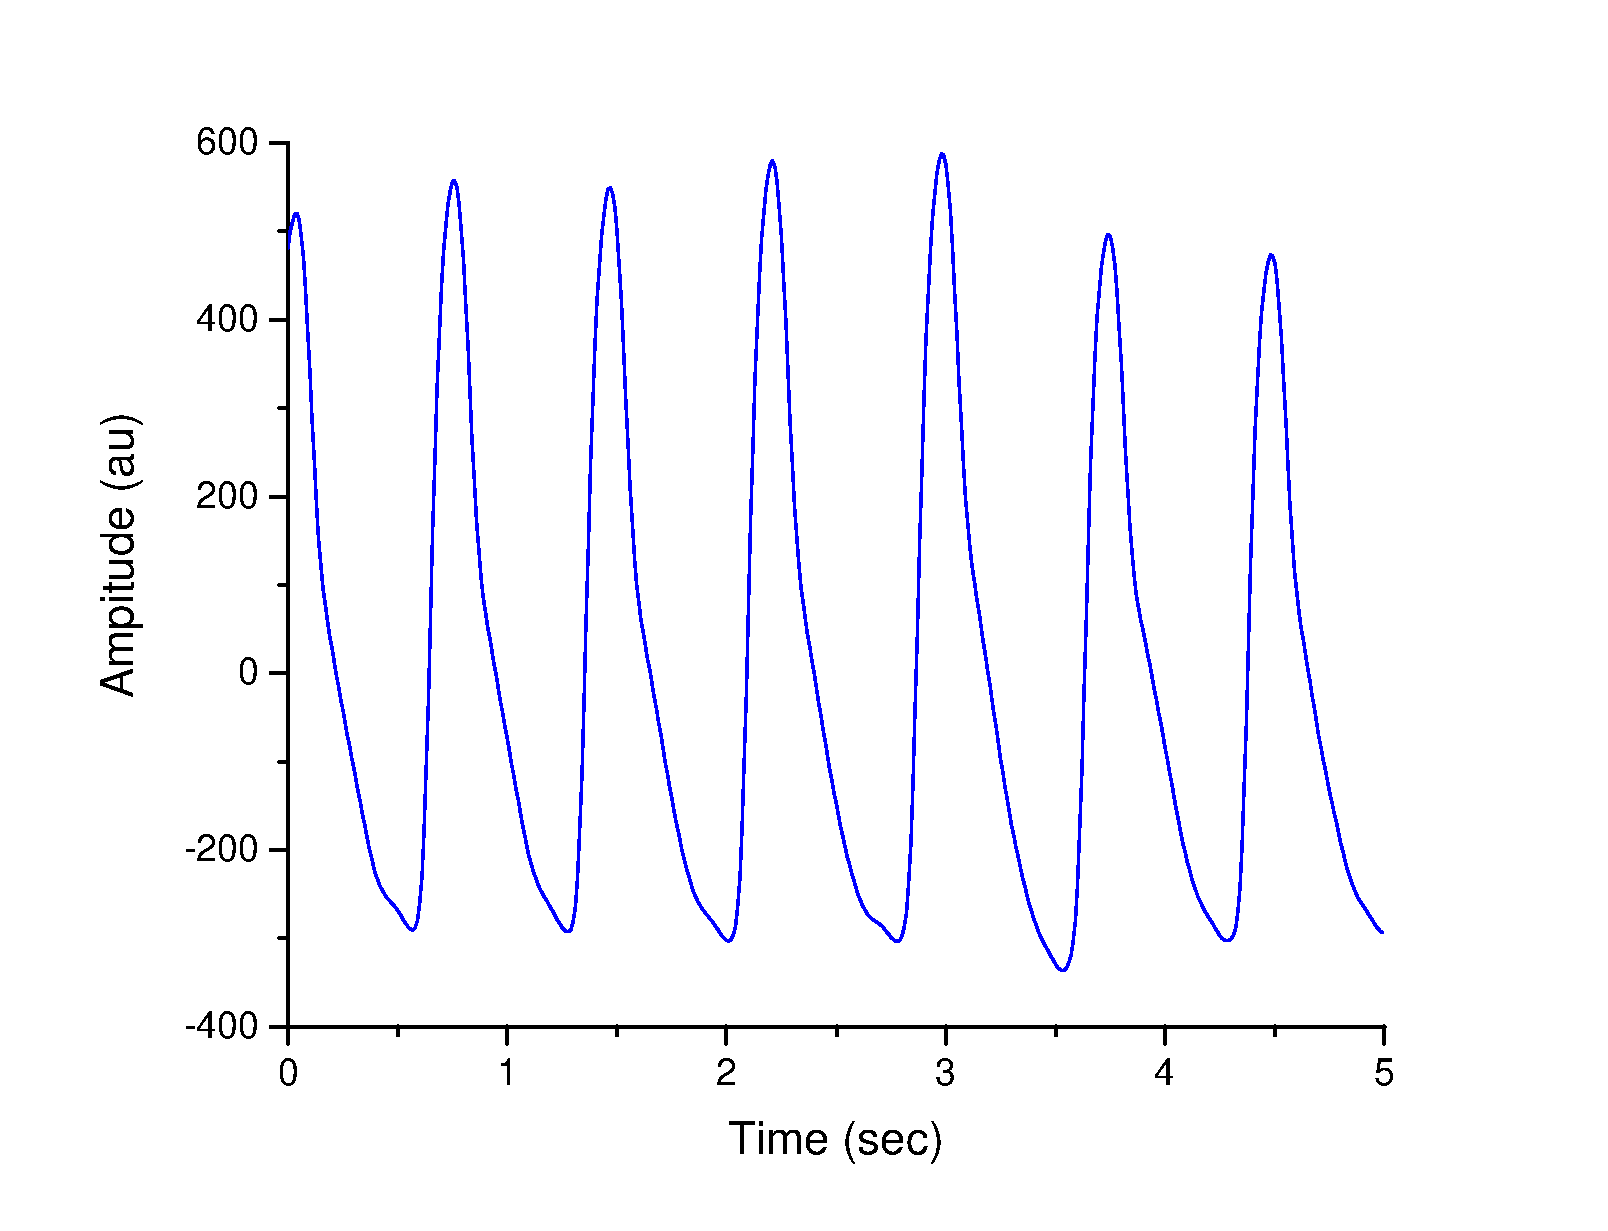
\includegraphics[width=6cm]{pulse_preprocess/after}
    }
    \caption{\label{fig:filter}平滑滤波前后PPG信号对比}
\end{figure}

\subsection{波形检测}
脉搏波波形的正确检测是后续所有特征计算的基础,因此,PPG波形检测算法的准确性及抗干扰能力显得尤为重要。传统的检测算法一般都是对波形进行一次性检测,然后再人工判别检测的准确性。
这种检测算法在应对较为复杂的信号时检测性能有所欠佳。
本小节借鉴了计算机科学领域的机制与策略分离的设计思想,
改进了上述PPG波形检测流程,提出了一种新型PPG波形检测算法,即初筛-复核-投票(Screen-Check-Vote,SCV)算法。

机制与策略分离是计算机系统领域的一项重要设计原则,被广泛应用于一系列资源分配问题(如CPU调度、内存分配、服务质量)以及软件抽象的设计等问题中\cite{Wulf1974,Levin1975,Brinch2001}。
这里的机制可以理解成决定如何做(how),而策略则决定具体做什么(what)。
SCV算法在对PPG波形进行检测时,充分利用“宽进严出”的筛选原则,预先设计了初筛、复核及投票等机制,而对每个机制下具体使用的策略不做过多限制,可有效增强对复杂信号的处理能力、提高算法的检测准确度,
同时极大地保证了算法的适配性与调整的灵活性,这一过程如\autoref{fig:detect}所示。
\begin{figure}[htbp]
    \centering
    
\includegraphics[width=\linewidth]{pulse_preprocess/detect}
    \caption{\label{fig:detect}SCV算法检测流程示意}
\end{figure}

在本研究中,SCV算法主要依据PPG波峰的局部最大值原理进行波形初筛,引入了针对PPG波形的多标准二次复核与最终决策确认机制以减少错检发生的概率。
所有初筛得到的“可疑波形”经特定标准复核后均会得到基于该标准的一个输出判定结果。由检测算法的决策模块负责对多个标准的复核结果进行裁决判定,将“可疑波形”判断识别为正确波形或错检干扰段。
以下是各个机制下使用策略的具体介绍。

一、波形检测

波峰与波谷是脉搏波的最基本特征点,也是检测波形其他特征点的基础。顾名思义,波峰是特定PPG波形内的最大值,在其左邻域内PPG幅值单调递增,右邻域内PPG幅值单调递减,则显然波峰与波谷必然是原始数据中的局部极大值与局部极小值点。
故对PPG波形特征点定位可按以下步骤进行。

1. 波峰定位

计算并遍历原始信号的一阶导数$X^{'}$,若出现$X_i^{'}\ge 0$且$X_{i+1}^{'}\le 0$,则说明出现了极大值。此时,定义时长一长一短的两个搜索窗,分别以当前数据点为窗中心,向前后双向检测并返回窗内最大值的位置。
若两个搜索窗的返回结果一致,则说明返回值就是一个波峰点。为防止同一波峰被多次检测,只有与上一成功检测的波峰位置点不同返回值才会被加入波峰缓存数组$Peaks$中。

在实际检测时,常会出现一阶导数在某邻域内多次出现过零点,导致多个极大极小值连续出现。为避免连续调用搜索窗、提高算法效率,本研究针对性进行了以下剪枝优化设计:

\Rnum{1}.采用中心对称搜索窗

窗口进行最大值搜索时是以当前搜索位置中心对称前后双向搜索,实际当第一个过零点出现时,这一邻域内的所有极值点均已被检索过,得到的局部最值已经是该邻域内最值。

\Rnum{2}.合理设置搜索窗时长

结合正常波形的形态特点,本研究将搜索窗时长分别设置为0.1s与0.3s。前者可以直接剔除掉时间跨度过小的局部极值,后者是基于此前PPG波峰与其重博峰时间间隔的经验值,可以保证重博峰点不会被误检为整个波形的波峰。

\Rnum{3}.搜索窗步进值策略调整

若长窗在当前位置$C$以中心沿时间轴延伸方向找到了局部极大值的坐标$L$后,下一次的搜索窗位置可直接从该$L$处开始。具体而言,若此时短窗返回结果$S=L$,则返回值必然是检测得到的波峰位置$P$,下次搜索可直接从波峰后开始;若$S\ne L$,
此时从$C$至$L$再进行搜索已经不可能再更新$L$坐标。而由于长窗搜索必然包含短窗,故下次搜索也可以同样调整检索位置从$L$处开始。

2. 波谷定位

一般而言,在波峰的位置确定之后,波谷的定位相对简单,一种可行的处理思路是将两个连续波峰之间的最小值定义为PPG波形的波谷。但该思路对复杂信号的处理效果欠佳,因为这种处理思路已经默认了所有的波形均已被正确无误地检测出来且
波形之间有连续性,即任意两个波形之间不存在其他干扰段。
因此,本研究对波谷的定位仍然按照先寻找定位再二次确认的思路进行,其中,波谷在满足上述条件的基础上,需要进一步满足其出现位置必须在这两个波峰之间的后半段。
此步得到的PPG波谷位置也被保存至缓存数组$Troughs$中,这一过程如\autoref{alg:troughs_detect}所示。
\begin{breakablealgorithm}
    \caption{PPG波形波谷定位检测}
    \label{alg:troughs_detect}
    \begin{algorithmic}[1] %每行显示行号
        \Require 待检原始数据数组$Points$,原始数据的一阶差分数组$D$,波峰数组$Peaks$
        \Ensure 正常形态下记录脉搏波波谷位置的数组
        \Function {DetectTroughs}{$Points, D, Peaks$}
            \State 初始化$Troughs$
            \For{$i\gets 0,Peaks.length()-1$}
                \State $leastX \gets (Peaks[i].x + Peaks[i+1].x )/2$
                    \For{$j \gets Peaks[i+1].x)-1, leastX$}
                        \If {$D[j-1]<0 \And D[j]\le 0$}
                            \State $lastT \gets Points[j]$
                            \State \textbf{break}
                        \EndIf
                    \EndFor
                \State $Troughs \gets lastT$
            \EndFor
            \State \Return{$Troughs$}
        \EndFunction
    \end{algorithmic}
\end{breakablealgorithm}

3. 完整波形确认

前两步已经分别得到了原始信号中所有波峰与波谷点,此时仅需按照波谷(start)——波峰(peak)——下一波谷(end)组合成完整波形即可。针对某些异常信号,\autoref{alg:troughs_detect}会出现两波峰之间无法有效检出波谷的极端情况。
因此,有必要对可能组合成完整波形的波峰波谷再次进行检查。本研究以PPG波形必定符合一定的时间规则对上述波峰波谷进行了“组合”。参考以往研究对PPG波形对经验统计,最终组合的波形起点与波形终点间期$P_{S2E}\ge 0.4s$,
波形峰值点与波形终点间期$P_{P2E}\ge 0.3s$。换言之,最终经过确认的波形的间期必定在上述数值内。

4. 其他特征点定位

由于波形其他特征点的定位依赖于波形的正确检测,因此,初筛阶段不做除波峰波谷外的其他特征点检测。这些特征点的检测被推迟到SCV算法检测完成后才进行。

二、多标准评估

上述PPG检测算法与此前的诸多研究中的算法性能接近,改进提高有限。具体而言,对质量高的PPG信号有着较好的检测效果,但对类似\autoref{fig:samplesignal}中的异常段仍难以避免错检漏检等情况的出现。
鉴于此,本研究引入了对PPG波形对二次审核评估机制,以进一步增加检测算法对各种干扰信号的检测能力、对畸变信号的识别判断能力。

如绪论中所述,PPG信号可以视为平稳随机信号的一种,短时间采样得到的有效PPG波形信号理应具有较高的相似性\cite{Qiu2012}。另外,有效PPG信号与干扰信号、畸变信号在形态特征、统计特征方面均存在较大差异,存在设计算法实现自动区分的理论可行性。
基于以上前提,为使具有且仅具有PPG波形一般特征的初筛“可疑波形”可以通过复核评估,本研究特设计并提出了以下复核标准:

1.能量与功率标准

易知脉搏波的相对幅值$A$是采样时间$t$的函数,将其表示为$A(t)$。参考信号与系统中对信号能量的定义\cite{Alan2019}
\begin{equation}
    \label{equ:energy}
    E=||f(t)||^2=\int_{-\infty}^{+\infty}{|f(t)|^2}\,d t
\end{equation}
类似地,单个PPG信号的能量可表示为
\begin{equation}
    \label{equ:ppge}
    E=\sum_{t=t_{start}}^{t_{end}}|A(t)|^2
\end{equation}
同理可得该PPG波形在其持续时间内的平均功率为
\begin{equation}
    \label{equ:ppgp}
    P=\frac{E}{t_{end}-t_{start}}=\frac{\sum_{t=t_{start}}^{t_{end}}|A(t)|^2}{t_{end}-t_{start}}
\end{equation}
能量与标准标准基于PPG波形在原始采集数值上,即PPG信号中交直流信号成份总和(AC与DC)的相似性。若所有初筛波形的功率求其均值,可得筛选波形的平均功率$P_{mean}$。
本研究规定通过能量标准复核的波形其功率必须在$P_{mean}$的一定倍数区间内$[0.4 \cdot P_{mean},1.8 \cdot P_{mean}]$。

2.方差与标准差标准

若原始PPG信号中DC成份波动较大(如基线严重漂移),会使部分波形功率数值偏离上述正常$P_{mean}$合理倍数区间,导致这部分波形被能量与功率标准错误识别为干扰。因此,本研究引入了方差与标准差标准以重点关注PPG波形AC成份的相似性。
若将特定PPG波形持续时间内所有采样点均值定义为$\mathop{A} \limits^-$,则该波形的标准差可表示为
\begin{equation}
    \label{equ:ppgstd}
    S=\sqrt{\frac{\sum_{i=1}^{n}{(A_i-\mathop{A} \limits^-})^2}{n}}=\sqrt{\frac{\sum_{i=1}^n{A_i}^2}{n}-{\mathop{A} \limits^-}^2}
\end{equation}
类似地,可以计算所有初筛波形的标准差均值为$S_{mean}$。本研究规定通过标准差复核的波形其相应数值必须在$S_{mean}$的一定倍数区间内$[0.4 \cdot S_{mean},1.8 \cdot S_{mean}]$。

3.时间关系标准

时间关系标准是对PPG波形间期、波形上升支与下降支及重博波峰相关特征时长间期做出对限定,是所有合格波形筛查所共有的一般范式。

由于时间标准通常与特征点的联系紧密,部分时间标准已经在
波形定位阶段得到了应用。如波形检测阶段,搜索窗的窗长已经限定了重博波峰与主波峰间期$T_{P2R}\ge0.3s$;
完整波形在进行确认时也限定了波形周期$T_{S2E}\ge 0.4s$、下降支时长$T_{P2E}\ge 0.3s$。
若参照心率定义,将一分钟中内有效脉搏波的数量规定为脉率(Pulse Rate,PR)。那么,原则上该算法可对$PR \le 150$的原始脉搏波数据进行波形检测。

此外,由于血管回流作用,PPG波形的下降支较上升支更长,因此,波峰位置必然在整体的前半段,在此基础上,波峰在波形中的位置可用下式表征
\begin{equation}
    \label{equ:timestd}
    PP = \frac{t_{end}-t_{start}}{t_{peak}-t_{start}}
\end{equation}

为排除异常极值的影响,本研究在计算出所有波形的$PP$数值并按升序排列后,取前$20\%$-$80\%$的波形计算其均值${PP}_{mean}$。
本研究规定通过基线偏移复核的波形其$PP$数值必须在${PP}_{mean}$的一定倍数区间内$[0.8 \cdot {PP}_{mean},1.2 \cdot {PP}_{mean}]$。

4.基线偏移标准

基线偏移最值标准是对PPG波形的起点与终点幅值差异程度的衡量。若两者的差值过大说明基线漂移严重,而这往往意味着波形处于一段较强的干扰中,具有较大的信号畸变可能,如\autoref{fig:samplesignal}所示。
若规定PPG波形起点与终点中幅值的较大的为$A_G$,较小值为$A_L$,同时规定$A_P$、$A_S$与$A_E$分别为波形波峰幅值、起点幅值与终点幅值,则基线偏移程度可用下列公式衡量
\begin{equation}
    \label{equ:baselinestd}
    \left \{
    \begin{aligned}
        \delta B &=A_G-A_L \\
        \Delta B &=\frac{A_G-A_L}{A_P-A_L}=\frac{\delta B}{A_P-A_L}\\
        \Delta B' &=\frac{A_P-A_S}{A_P-A_E}
    \end{aligned}
    \right.
\end{equation}
其中,$\delta B$是对偏移的绝对值的衡量,$\Delta B$与$\Delta B'$则是对偏移程度归一化的衡量。

由于正常PPG波形$\Delta B$数值较小,而基线严重漂移时$\Delta B$数值显著增大,甚至达到正常波形的数十倍以上。
为消除漂移波形对最终均值的影响,本研究在计算出所有波形的$\Delta B$数值并按升序排列后,取前$80\%$的波形计算其均值${\Delta B}_{mean}$。
本研究规定通过基线偏移复核的波形其$\Delta B$数值必须在${\Delta B}_{mean}$的一定倍数区间内$[0,10 \cdot {\Delta B}_{mean}]$,
类似地,$\delta B$数值必须在${\delta B}_{mean}$的一定倍数区间内$[0,8 \cdot {\delta B}_{mean}]$。
而对$\Delta B'$而言,计算均值再排序的意义不大,由于$A_S$与$A_E$在\autoref{equ:baselinestd}中的对称性,最终数值的上下限必定互为倒数关系,本研究规定的倍数区间为$[0.5,2]$。

5.其他标准

目前为空,待补充。
由于不同人群、不同采集设备、不同采集环境下采集得到的PPG信号可能形态上千差万别,与之对应的干扰信号也往往不尽相同。上述标准仍有不足以甄别区分有效信号与无效干扰的可能。
故在此特保留其他标准占位,供后续研究视情况开发设计新标准从而进行功能性拓展。

三、投票决策

当初检波形经过上述PPG评估标准后,均会生成一定的输出,即基于当前标准判断的正确检测波形或错检干扰。为获取最终的评判结果,需要综合以上多个评估标准的输出,
形成最终的裁定。本研究借鉴了机器学习领域中集成学习中的投票策略(voting)来完成这个裁定过程,常见的策略有绝对多数投票法、相对多数投票法及
加权投票法等$f$\cite{Zhou2016}。
在实际处理PPG波形的复核时,会出现某些特定的标准的输出组合即可直接判断波形是否异常的情况。
另外,标准功率与标准差在定义上就有着极高的相似性,实际检测结果也十分相近,在与其他标准综合决策前有进一步调整压缩的可能与必要。
基于上述考虑,本研究最终对加权投票的策略进行了一定程度的改良如\autoref{tab:voting}所示。

上文介绍的能量标准、标准差及方差标准等被压缩成三个新的综合标准。
综合标准在进行计算时,使用原标准基于波形是否异常的0或1的输出直接进行数值加法,而非基于各项原始数值。在进行加权投票时,\autoref{tab:voting}中综合标准的类概率是基于本实验数据得到的经验数值,综合标准加权
计算结果超过0.5的波形会被判断为干扰。
\begin{table}[htbp]
    \centering
    \zihao{-4}
    \caption{\label{tab:voting}经改良的加权投票法}
    \begin{tabularx}{\linewidth}{X<{\centering}X<{\centering}cX<{\centering}}
        \toprule
        \textbf{综合标准}&\textbf{计算方式}&\textbf{类概率权重}&\textbf{直接判为异常条件}\\
        \midrule
        能量类标准&     $ES=P+S$               &0.3& $ES =2$ \\
        时间类标准&     $TS=PP$&0.2&/\\
        基线类标准&     $BS=\delta B+\Delta B+\Delta B'$&0.5& $BS\ge 2$  \\
        \bottomrule
    \end{tabularx}
\end{table}

四、检测算法性能评估

SCV算法并不保证检测波形在时间上的连续性,在初筛阶段就会忽略明显不符合时间标准的PPG数据段,而肉眼可辨别的明显异常的波形也在复核阶段被检测出来。
此外,由于实际中对异常的波形的漏检的代价远高于对正常波形的漏检,因此,SCV算法在设计时便对异常波形及其前一个波形一并视为异常处理,这可能会导致某些漏检的发生。
为精确评估本研究提出的PPG波形的SCV算法的性能表现,这里以本次研究得到的实验数据及公开数据库的PPG数据分别对其进行了测试。

1. 基于本次实验数据

如第二章中所述,本次实验共采集到有效数据79条,经统计分析,最终得到有效PPG波形共计7864个。而使用SCV算法对其进行检测,结果显示,SCV算法共计错检波形26个、漏检波形7个,
整体的准确率高达$99.6\%$以上。
\autoref{fig:detect_details}给出了展现SCV算法优异的检测性能的一些典型案例。由于篇幅所限,更多典型案例可参见\pageref{fig:detect_details2}页附录A。
此外,\pageref{fig:detectcheck}页附录B也给出了展现SCV算法具体检测过程的一个详尽实例。
\begin{figure}[h]
    \centering
    \subfigure[\label{fig:c_cll}被试CLL的波形检测结果]{
        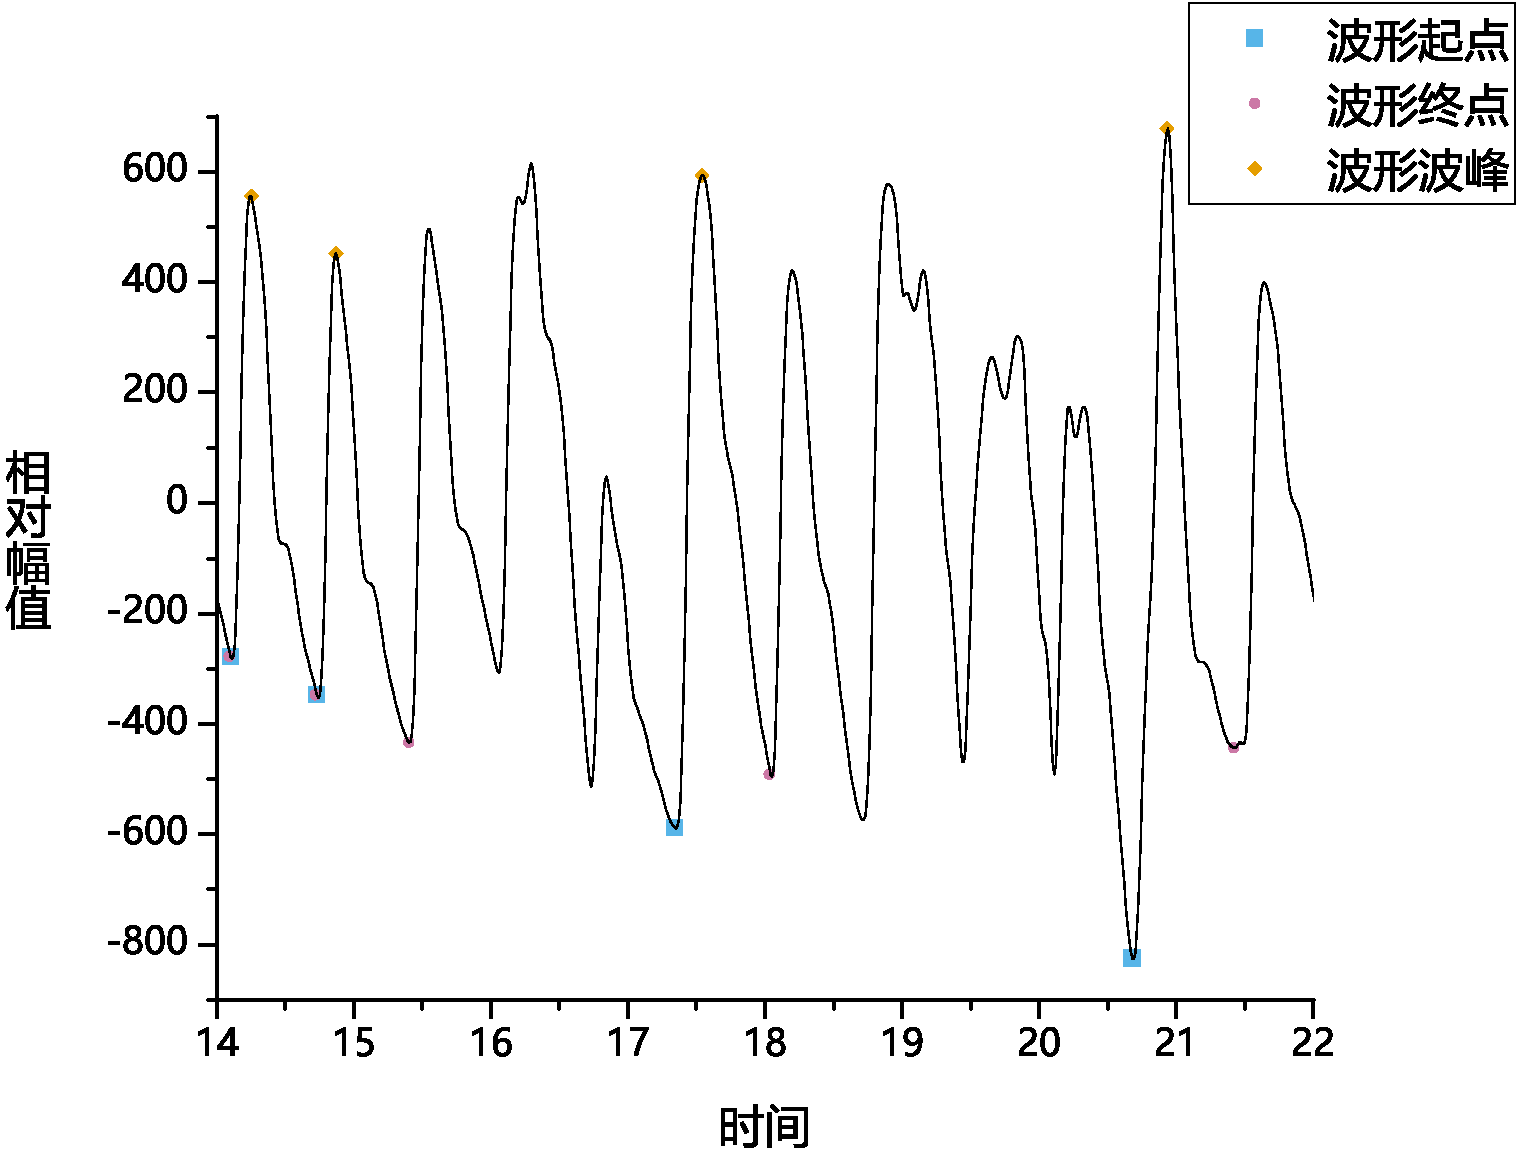
\includegraphics[width=7.5cm]{pulse_preprocess/check/cll}
    }
    \quad
    \subfigure[\label{fig:c_cww}被试CWW的波形检测结果]{
        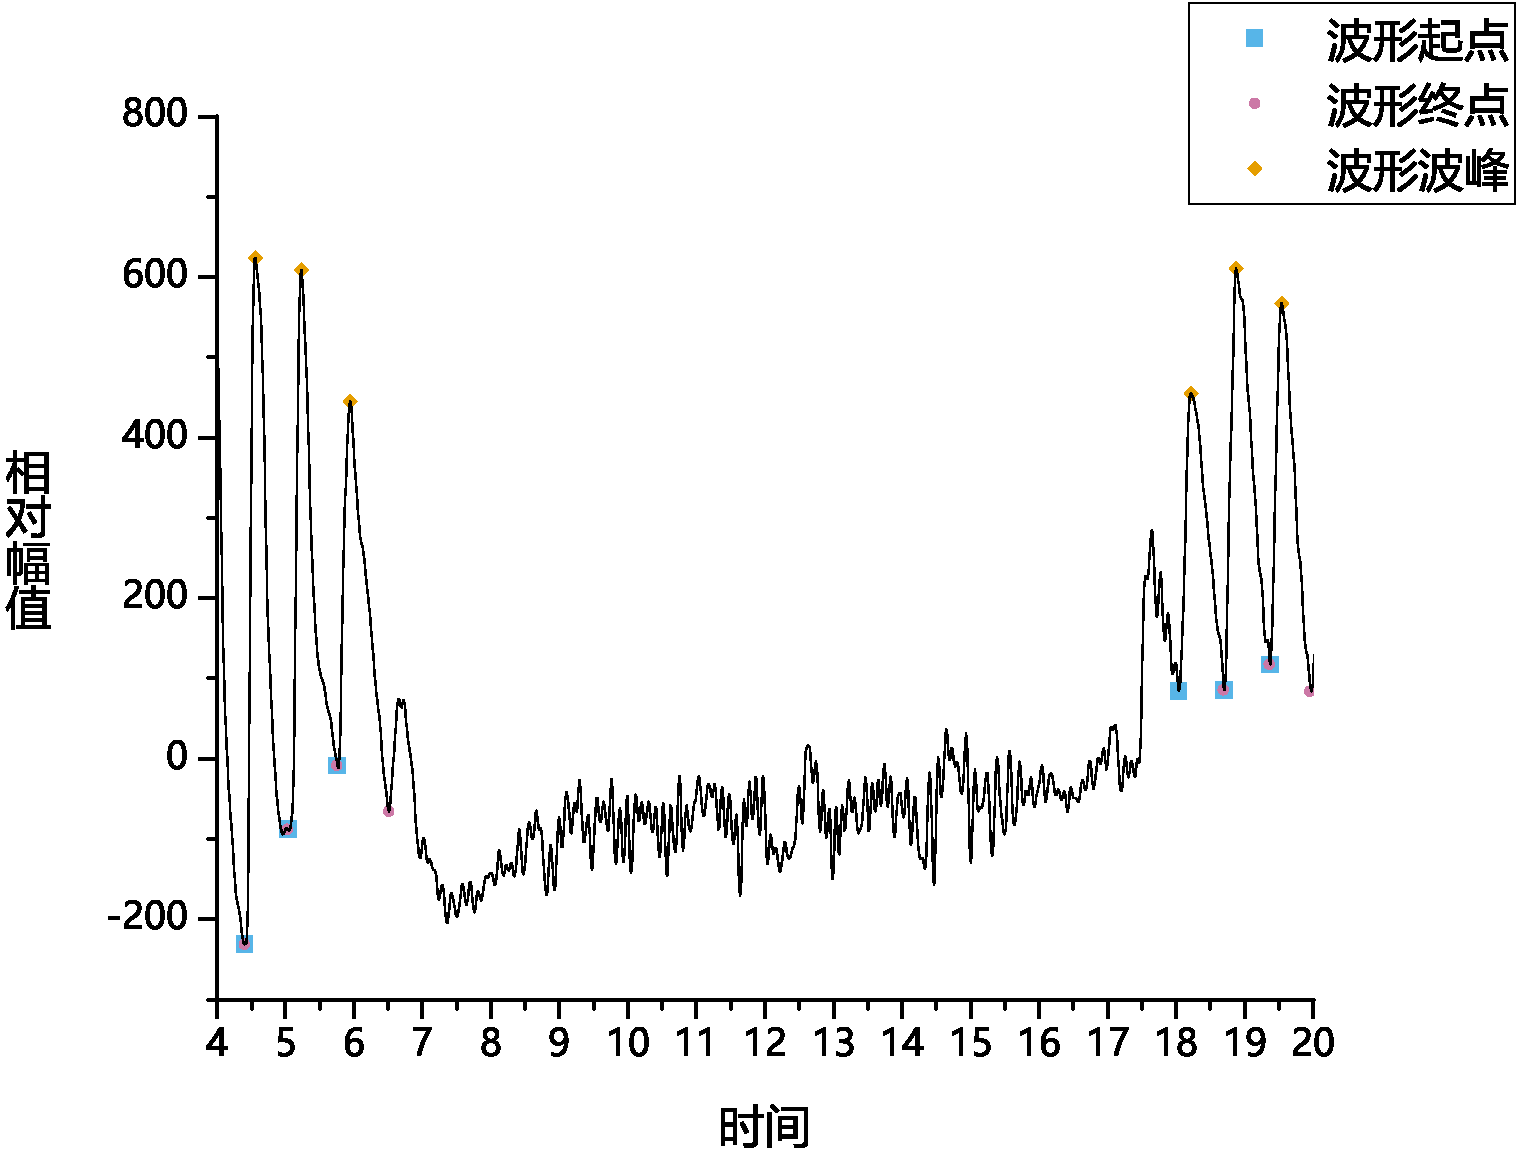
\includegraphics[width=7.5cm]{pulse_preprocess/check/cww}
    }
    \quad
    \subfigure[\label{fig:c_flh}被试FLH的波形检测结果]{
        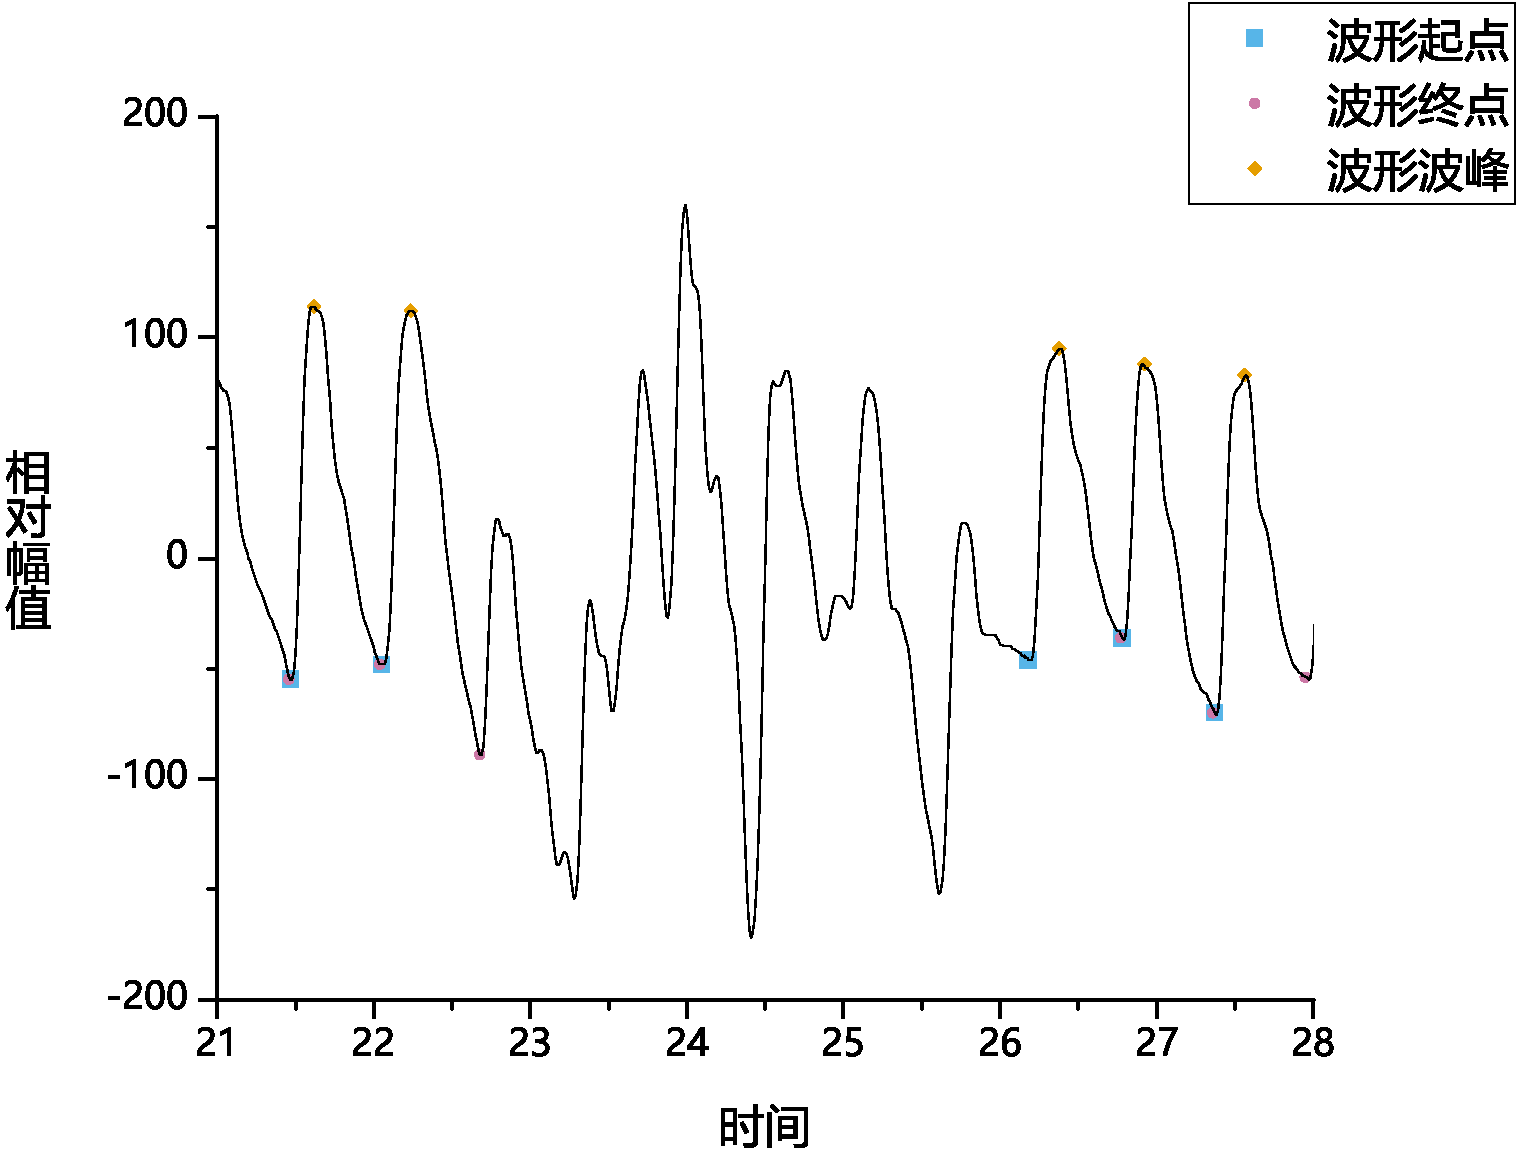
\includegraphics[width=7.5cm]{pulse_preprocess/check/flh}
    }
    \subfigure[\label{fig:c_ly}被试LY的波形检测结果]{
        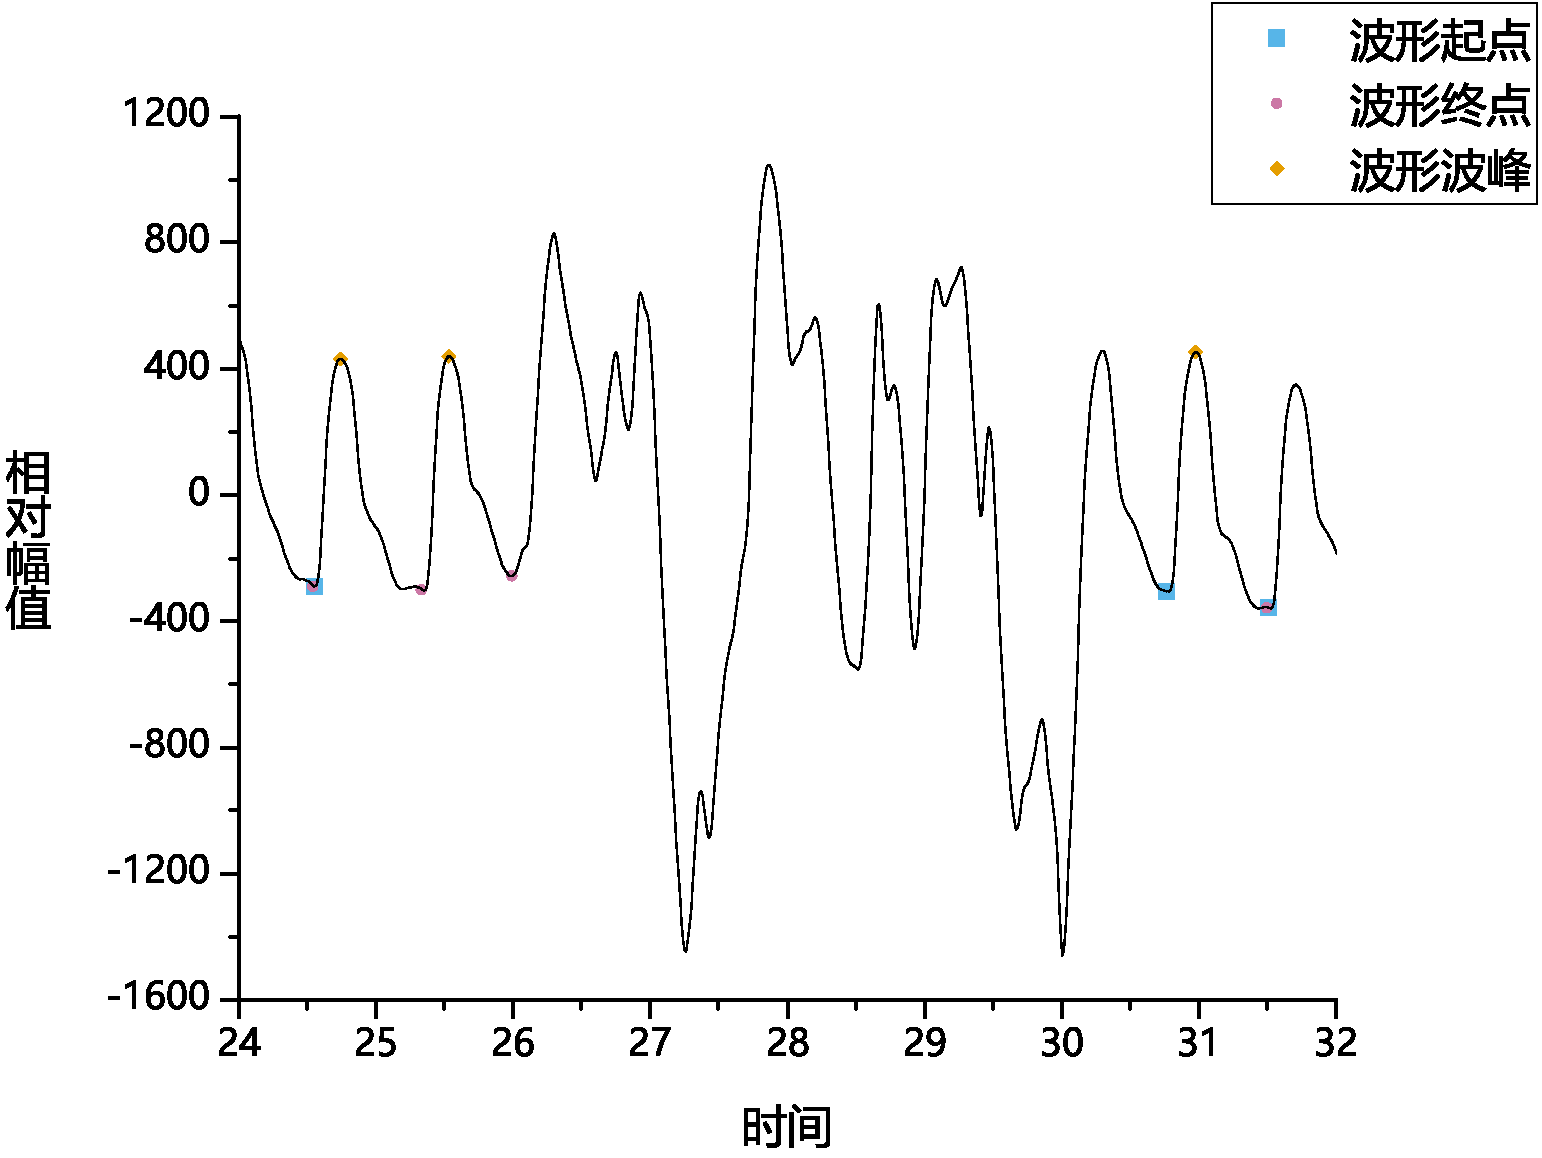
\includegraphics[width=7.5cm]{pulse_preprocess/check/ly}
    }
    \quad
    \caption{\label{fig:detect_details}SCV算法对复杂信号的检测效果示意}
\end{figure}

2. 基于公开数据库UCI-BP

MIMIC(Medical Information Mart for Intensive Care)是生物医学工程领域开源社区PhysioNet上最为知名的一个大型公开数据库\cite{mit2022,Goldberger2000,johnson2018mimic}。该数据库记录了2001年
至2019年期间贝斯以色列女狄肯斯医疗中心重症监护病房患者的相关数据,拥有超过40,000名患者的医疗健康数据记录\cite{johnson2018mimic}。目前,其最新版本为2022年6月发布的MIMIC-IV v2.0\cite{mimic4}。
2015年,Kachuee Mohamad等人在MIMIC-II的基础上进行了二次开发,他们在原始信号的基础上进行了一定的预处理与数据清洗,构建了无袖带血压估计验证数据集即UCI-BP数据集\cite{Kachuee2015,ucibp2022}。
UCI-BP数据集一共包含12,000条数据记录,每个记录包含脉搏波、有创动脉血压及心电等三通道数据,采样率均为$125Hz$,单条数据记录时长从1分钟内至10分钟不等。
UCI-BP数据集由于其出色的易用性而被广泛使用,本研究亦采用该数据集进行SCV算法的评估与验证。

由于UCI-BP数据记录量大,这里仅以该数据集来自\path{Part_1.mat}文件的前50条数据记录进行了SCV算法的性能评估。在不调整此前SCV算法涉及的各参数的基础上,使用SCV算法这部分数据其进行检测验证。
最终得到有效PPG波形共计17562个,而错检波形仅有50个,整体的准确率高达$99.7\%$以上,其中,共有35条数据记录实现了$100.0\%$的检测率,占参与验证的数据量的$70.0\%$。
这部分数据的统计详情及典型检测案例参见\pageref{tab:ucibp_details}页附录C。

值得一提的是,由于UCI-BP数据集本身包含了某些重症监护下的特殊病人,部分PPG数据异常畸形,已经明显异于正常波形,SCV算法对这部分异常数据的检测能力有限(或者说SCV算法“成功地”将这些畸形波形识别为异常),
如\autoref{fig:ucibp_abnormal}所示。
\begin{figure}[h]
    \centering
    \subfigure[\label{fig:c_0179}编号0179原始数据波形(局部)]{
        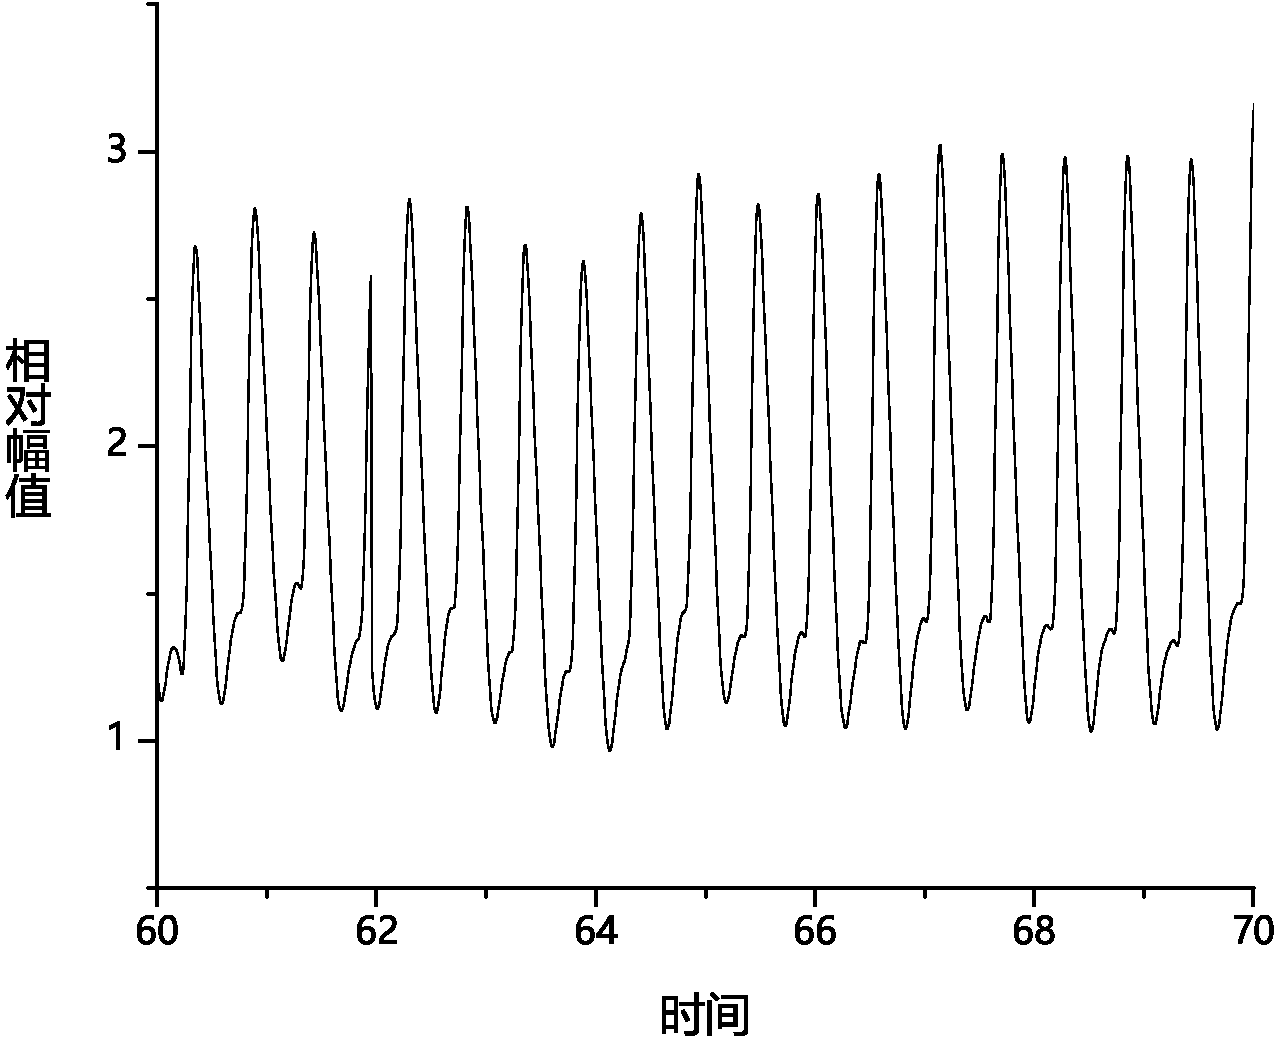
\includegraphics[width=7.5cm]{pulse_preprocess/check/0179}
    }
    \quad
    \subfigure[\label{fig:c_0533}编号0533原始数据波形(局部)]{
        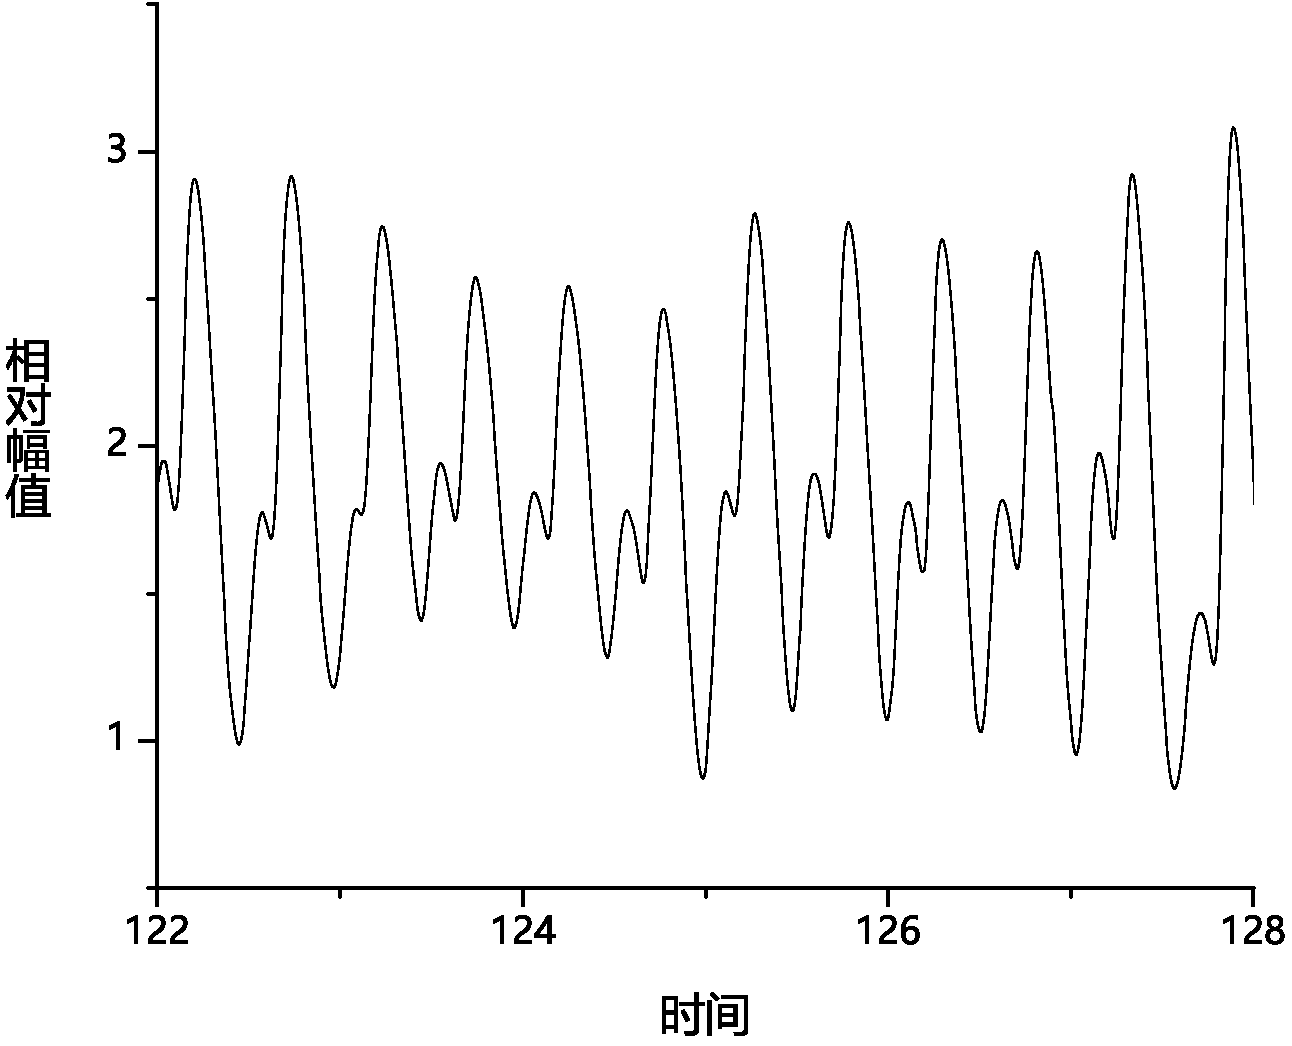
\includegraphics[width=7.5cm]{pulse_preprocess/check/0533}
    }
    \quad
    \caption{\label{fig:ucibp_abnormal}UCI-BP数据库中畸形信号示意}
\end{figure}

五、综合评价

综上所述,SCV算法在PPG波形检测问题上的检测性能优异,抗干扰能力强。其中,SCV算法复核阶段采用的功率、标准差、时间与基线等四类复核标准
设计合理,均可按照设计初衷识别出特定的异常干扰段,达到数据分析预期。另一方面,由于SCV算法整体采用模块化设计,各模块均具有良好的拓展性,
不论是对已获取的数据进一步提高检测性能,还是对新的存在特定干扰待检信号的准确检测,SCV算法都有着可进一步挖掘的潜力。

\subsection{重搏波与切迹检测}
重博波是脉搏波最具标志性的波形特征之一,其波峰与切迹的检测是一个完整的脉搏波检测算法必不可少的定位项之一\cite{Wang2012}。但在实际应用中,并不是每个人的PPG信号都有着明显的重搏波,特别是当被试出现外周阻力增加、血管壁弹性下降的情况后\cite{mmt}。
此时,随着PPG波形向外周传播,尖锐的重搏波切迹(incisura)常会变形甚至丢失,退变成一简单拐点,甚至重搏波波峰都会在下降支中不显著,导致最后无法从采集得到的信号中对两者直接进行精准定位,如\autoref{fig:samplesignal}所示。

由于本次实验数据中有大量重博波及切迹不明显的信号段,因此本研究借鉴了王选等人于2012年提出的一种基于曲率$K$(curvature)的定位算法对上述特征点进行检测\cite{Wang2012}。
该算法的核心思想是PPG信号在切迹退化成的变形点的邻域内具有最大的曲率值,如\autoref{fig:incisura}所示。
数学中将一般曲线函数在点$(x,y)$处的曲率$K$定义为
\begin{equation}
    \label{equ:curvature}
    K=\frac{|y^{''}|}{{(1+{y^{'}}^2)}^{3/2}}
\end{equation}
其中,$y^{'}$与$y^{''}$分别是曲线函数在该点的一阶导数与二阶导数。王选等人的算法检测过程可概括如\autoref{alg:incisuras_detect}所示\cite{Wang2012}。
\begin{figure}[htbp]
    \centering
    \subfigure[重博波明显的PPG波形]{
    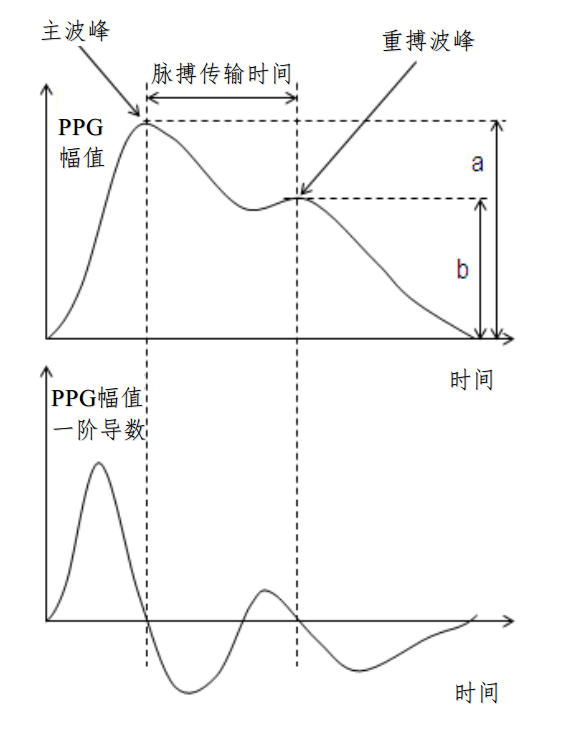
\includegraphics[width=5.5cm]{pulse_preprocess/ri1}
    }
    \quad
    \subfigure[重博波不明显的PPG波形]{
    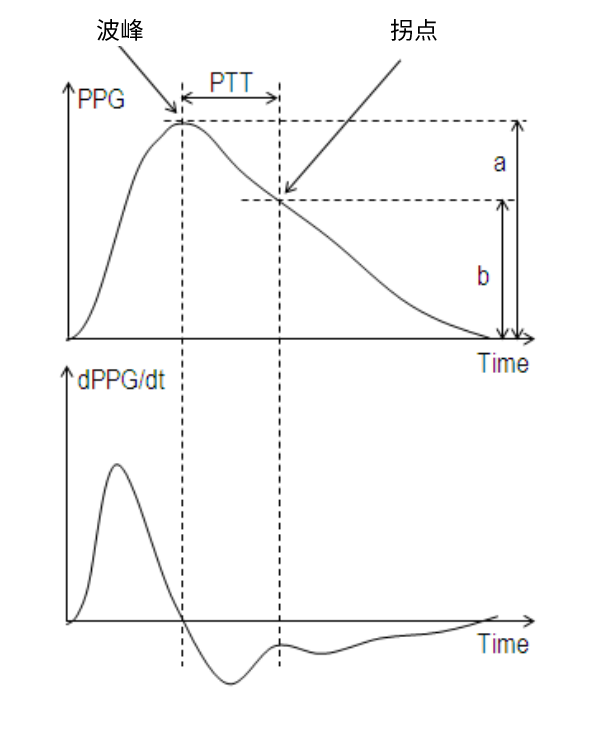
\includegraphics[width=5.5cm]{pulse_preprocess/ri2}
    }
    \caption[重搏波及切迹定位原理]{\label{fig:incisura}重搏波及切迹定位原理\cite{Wang2012,Su2014}}
\end{figure}

\begin{breakablealgorithm}
    \caption{PPG波形切迹定位检测}
    \label{alg:incisuras_detect}
    \begin{algorithmic}[1] %每行显示行号
        \Require 原始数据数组$Points$,检测完毕的波形$pulse$,原始数据的一阶差分数组$D$
        \Ensure 当前波形的切迹位置
        \Function {DetectIncisura}{$Points, pulse, D$}
            \State $s \gets pulse.peak.x + \frac{3}{10}(pulse.trough.x-pulse.peak.x)$
            \State $e \gets pulse.peak.x + \frac{9}{10}(pulse.trough.x-pulse.peak.x)$
            \State \Comment 切迹可能出现的位置为波形的下降支中后部分。
            \State $M  \gets \Call{Max}{$D[s],D[e]$}$
            \State \Comment 寻找到上述区间内一阶导数最大值点记为$M$。
            \If{$D[M] >0$}
                \State \Comment 下降支中存在明显的重搏波。
                \State $Incisura \gets \Call{Min}{Points[s],Points[M]}$
                \State \Comment 重搏波波峰即为点M至脉搏波终点之间的极大值点,切迹为脉搏波波峰至点M之间的最小值点。
            \Else
                \State \Comment 下降支一直单调下降,不存在明显的重搏波。
                \State $Incisura \gets \textproc{Min}({\Call{Curvature}{Points[M],Points[e]}})$
                \State \Comment 重搏波波峰定义为点M至脉搏波终点之间的曲率最大处,切迹定义为脉搏波波峰至点M之间的曲率最小处。
            \EndIf
            \State \Return{$Incisuras$}
        \EndFunction
    \end{algorithmic}
\end{breakablealgorithm}

\subsection{去除基线漂移}
由于呼吸干扰等原因,实际得到的PPG波形的两个波谷的幅值(即该波形的始末位置的幅值)很难保持一致。这种差异最终会导致PPG信号的基线出现波动漂移,如\autoref{fig:drift}所示。为满足后续特定PPG形态特征计算需求,
需要消除基线漂移的影响。此时可借助一种基于线性变换的思路完成相应处理。
\begin{figure}[htbp]
    \centering
    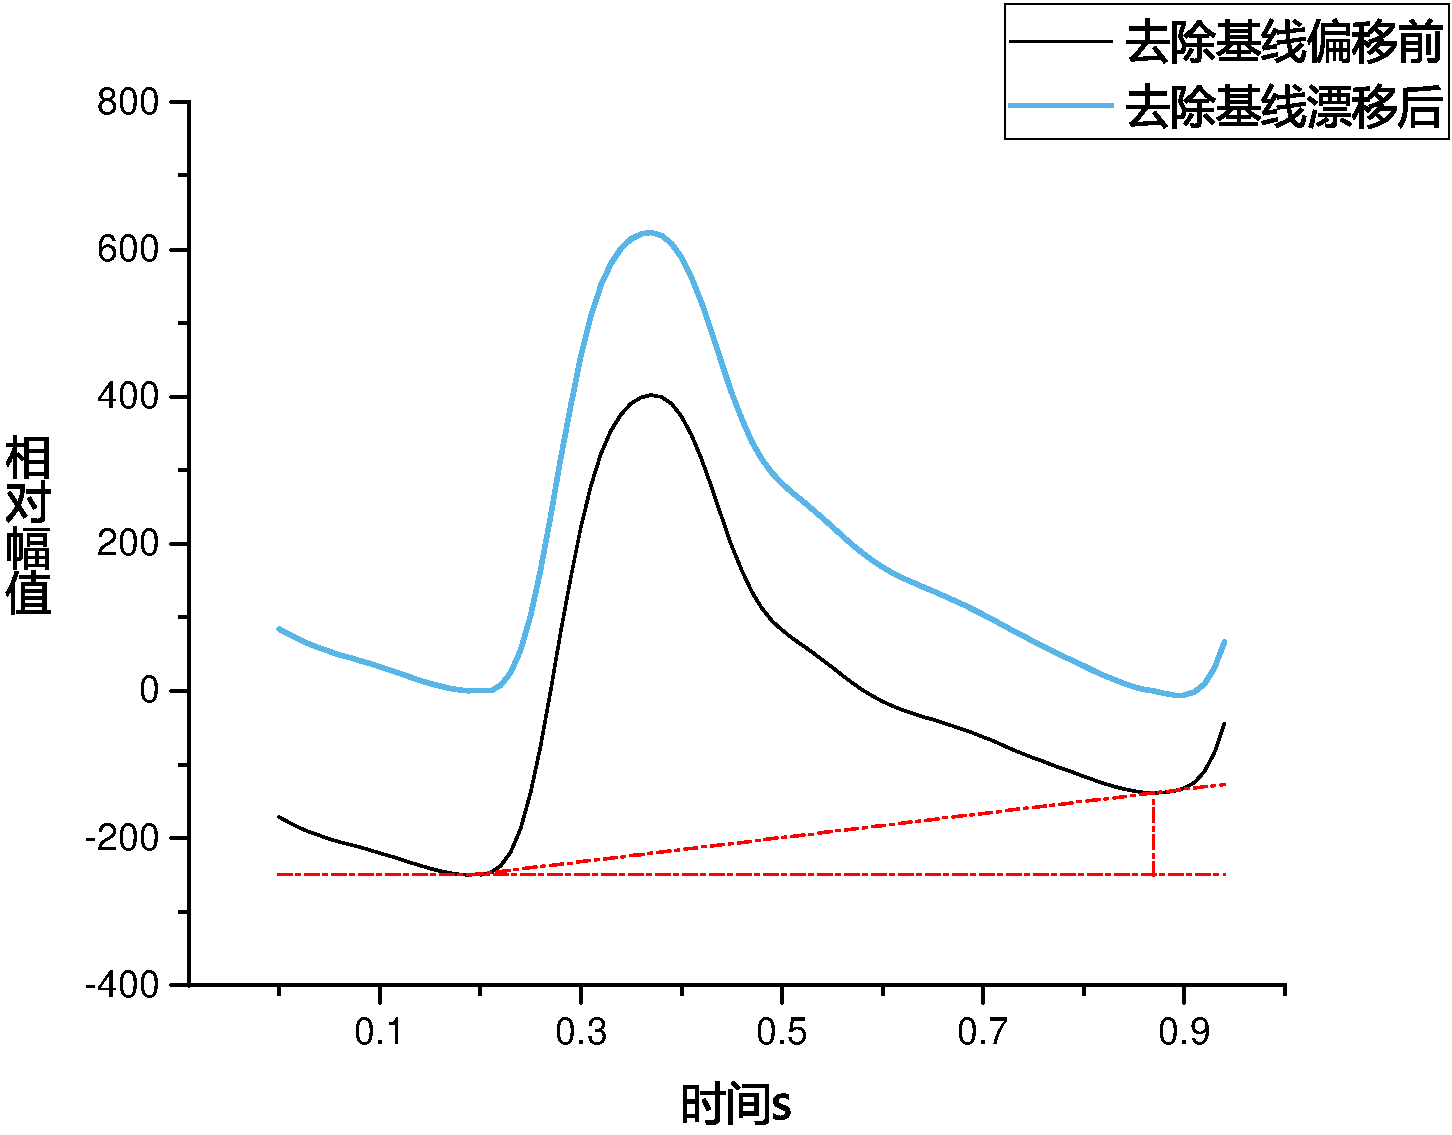
\includegraphics[width=.6\linewidth]{pulse_preprocess/baselineadjust}
    \caption{\label{fig:drift}基线漂移去除原理示意及处理前后对比}
\end{figure}

易知脉搏波的相对幅值$A$是采样时间$t$的函数,将其表示为$A(t)$。对任一特定波形,其起始点与终止点处对应的幅值可分别表示为$A(t_{start})$与$A(t_{end})$。
由于始末位置脉搏波幅值不等,则明显两者之间存在一条斜率$k \ne 0$的直线,其中
\begin{equation}
    \label{equ:linek}
    k=\frac{A(t_{start})-A(t_{end})}{t_{start}-t_{end}}
\end{equation}
则该直线上任意点即代表了在该时刻脉搏波波形与水平基线的偏移量,即
\begin{equation}
    \label{equ:liney}
    \Delta(t)=k(t-t_{start})+A(t_{start})
\end{equation}
此时,去除基线漂移后的脉搏波信号可标示为
\begin{equation}
    \label{equ:adjusta}
    A_{adjsut}(t)=A(t)-\Delta(t)
\end{equation}

\subsection{信号的重采样}
通常而言,脉搏波数据的采样率是固定不变的。但在某些情况下,原始数据采样率不能满足实际需求,在进行相应数据处理任务前需要先进行采样率调整。
如在本研究自行定义设计的多种新型脉搏波时域特征的计算时,经由GE B450设备导出的原始脉搏波数据的采集频率仅为100$Hz$,难以满足后续计算看,需要进行额外处理以提高信号采样率。
其中,减少抽样率的过程称为信号的抽取,也称抽样率压缩;增加抽样率的过程则称之为信号的插值,也即抽样率扩张\cite{Cheng2008}。信号的抽取与插值都会导致原始信号出现频谱迁移,即改变信号的频率成份\cite{Cheng2008}。

相对而言,信号的抽取过程更容易理解。若需要用整数$D$对$x(n)$进行抽取,以使抽样率降低到原始值的$1/D$,可按照每连贯的$D$个抽样中取出一个信号值。这样的处理称为整数$D$抽取\cite{Cheng2008}。
插值是抽取的逆过程,通过某些已知的数据点去推断一个(系列)特定的函数,使得所有已知数据点均在该函数图像上,从而去推断更多未知数据点,这一过程如\autoref{fig:spline}所示。若不考虑可能出现的信号失真,理论上
可以通过调整抽取与插值的数值对原始信号的采样率进行任意的调整。
\begin{figure}[htbp]
    \centering
    \subfigure[经过点(1,2),(2,1),(4,4)和(5,3)的线性样条]{
    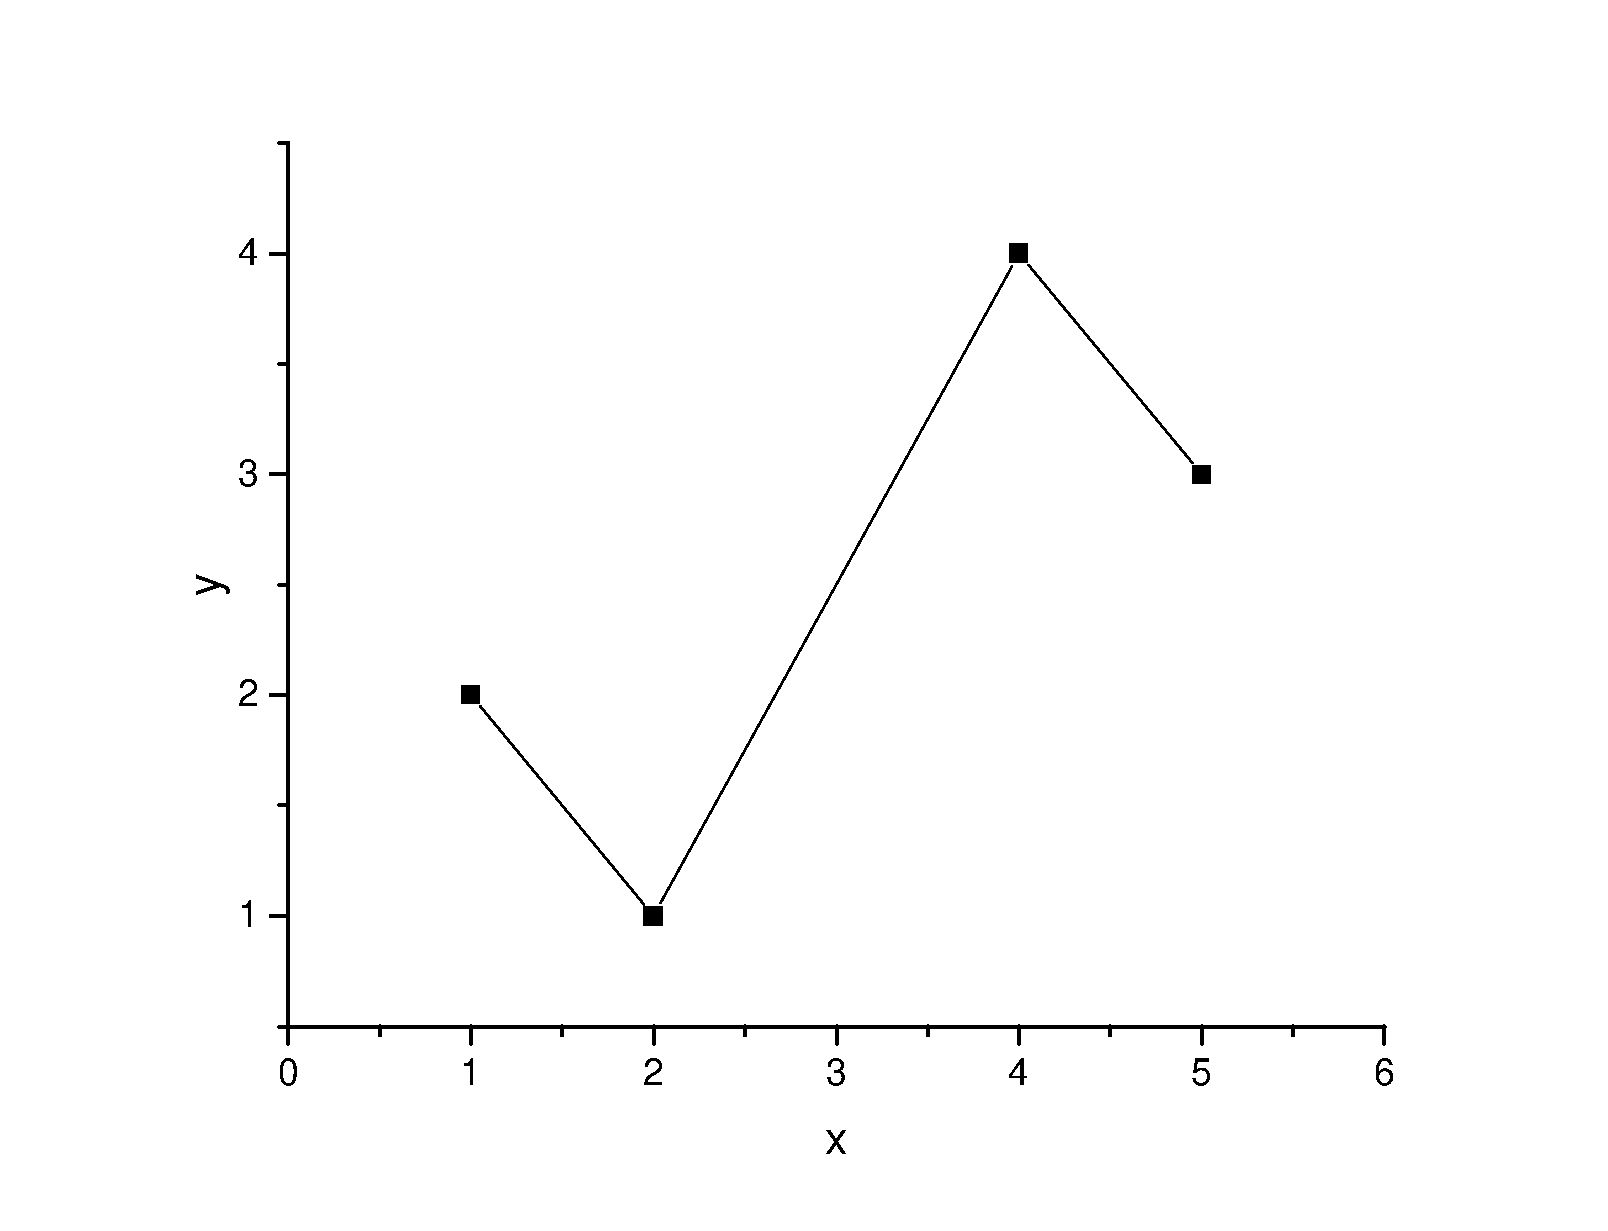
\includegraphics[width=5.5cm]{pulse_preprocess/spline1}
    }
    \quad
    \subfigure[经过相同点的一种可能的三次样条插值]{
    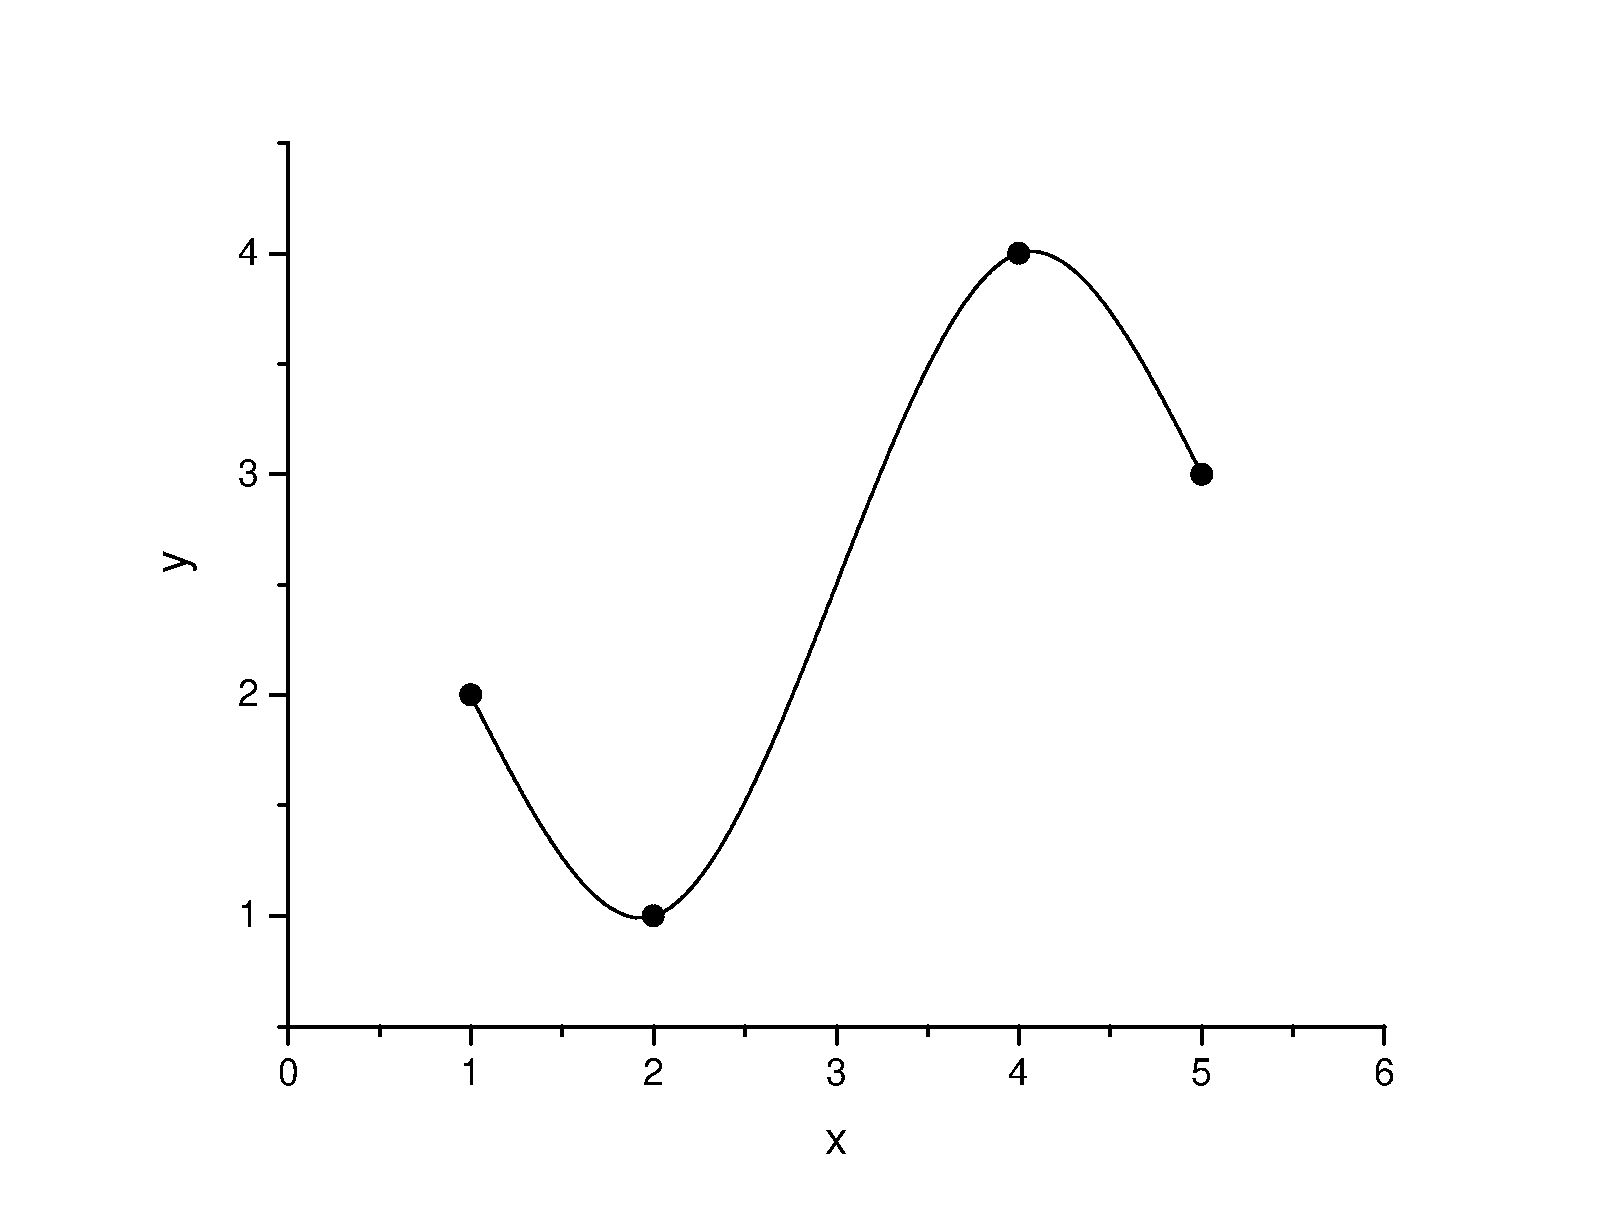
\includegraphics[width=5.5cm]{pulse_preprocess/spline2}
    }
    \caption{\label{fig:spline}经过4点的线性样条插值与三次样条插值对比}
\end{figure}

多项值插值与样条插值是插值最常用的两种算法\cite{Timothy2018,Carl2008}。多项式插值给出满足所有原始数据点的单一公式,由于此过程中仅涉及浮点数加法与乘法,可以很方便的在PC及嵌入式设备上实现,因而得到广泛应用。
而样条插值则使用多个公式来通过所有数据点,其中每个公式均为低阶多项式。三次样条插值是样条插值在工业领域应用最广泛的算法之一,可以得到光滑的拟合插值曲线。
具体而言,对原始数据点$(x_1,y_1),(x_1,y_1),\cdots,(x_n,y_n)$,三次样条的插值曲线$S(x)$在每两个数据分段区间$[x_i,x_{i+1}]$内均使用三阶多项式
\begin{equation}
    \label{equ:spline}
    S_{i}=y_{i}+b_{i}(x-x_{i})+c_{i}{(x-x_{i})}^2+d_{i}{(x-x_{i})}^3
\end{equation}
并保证每两个多项式在端点(即原始数据点)处不仅数值相等,相应的斜率与曲率均相等,即
\begin{equation}
    \label{equ:cubiccha}
    \left \{
    \begin{aligned}
        S_{i}(x_{i})&=y_i,&\text{i=1,$\cdots$,n-1}\\
        S_{i}(x_{i+1})&=y_{i+1},&\text{i=1,$\cdots$,n-1}\\
        S_{i}^{'}(x_{i-1})&=S_{i}^{'}(x_{i}),&\text{i=2,$\cdots$,n-1} \\
        S_{i}^{''}(x_{i-1})&=S_{i}^{''}(x_{i}),&\text{i=2,$\cdots$,n-1}
    \end{aligned}
    \right.
\end{equation}
使用微积分的定义,将\autoref{equ:spline}代入\autoref{equ:cubiccha}化简整理后,可以得到包含$3n-5$个独立方程的方程组。另一方面,由于每个局部$S_i$中有三个未知参数,一共有$3n-3$个待解参数,则此时由线性代数相关知识可知,该方程组有无穷多组解。
即此时可以构造处无穷多条通过所有数据点$(x_i,y_i)$的样条曲线。因此,需要添加额外的方程对样条曲线进行约束,一般的约束条件都是对样条左右端点处进行限定 ,常见的附加边界条件如\autoref{tab:splinekind}所示\cite{Timothy2018}。
\begin{table}[htbp]
    \centering
    \zihao{-4}
    \caption{\label{tab:splinekind}几种常见的三次样条端点条件}
    \begin{tabularx}{\linewidth}{X<{\centering}X<{\centering}}
        \toprule 
        \textbf{样条种类}&\textbf{端点条件}\\
        \midrule 
        自然三次样条&
        $
            S_{1}^{''}(x_{1})=0,
            S_{n-1}^{''}(x_{n})=0
        $
        \\
        曲率调整三次样条&
        $\left \{
        \begin{aligned}
            &S_{1}^{''}(x_{1})=v_1,&v_{1}\neq0\\
            &S_{n-1}^{''}(x_{n})=v_n,&v_{n}\neq0
        \end{aligned}
        \right.
        $
        \\
        钳制三次样条&
        $\left \{
        \begin{aligned}
            &S_{1}^{'}(x_{1})=v_1,&v_{1}\neq0\\
            &S_{n-1}^{'}(x_{n})=v_n,&v_{n}\neq0
        \end{aligned}
        \right.
        $
        \\
        抛物线端点三次样条&
        $
            d_1=0,d_{n-1}=0
        $
        \\
        非纽结三次样条&
        $
            d_1=d_2, d_{n-2}=d_{n-1}
        $
        \\
        \bottomrule
    \end{tabularx}
\end{table}

在补充\autoref{tab:splinekind}中的两个端点条件公式后,即可完成上述方程组求解,从而确定唯一的三次样条插值曲线。本研究中三次样条算法基于自然边界条件对PPG信号进行均匀插值\cite{ttk2021},使信号采样率被提高至2000$Hz$。
\subsection{数据标准化}
在上述各项预处理过程完成后,此时得到的PPG数据在波形幅值上仍然有很大的个体差异,即使对同一被试对象,其波形在幅值上也会有一定的波动。为消除个体差异对特定波形特征计算的影响,需要对脉搏波信号进行归一化处理。

时间标准化与幅值标准化是PPG标准化两类常见的方式\cite{mmt}。时间标准化的基本原理是将PPG信号进行分组并计算每组信号的平均心动周期,随后对每组内的PPG信号进行时间尺度上的缩放,使最终的总平均心动周期保持一致。
由于不同个体的时间尺度上的缩放比例不一致,很容易导致PPG信号波形发生畸变失真,严重影响后续特征计算。故本研究采取了幅值标准化的处理方式对PPG信号进行处理。

由第二章PPG信号光学采集的基本原理可知,PPG信号的波形幅值对不同个体而言并无实际的生理意义,这保证了对PPG信号幅值标准化的合理性。与去除基线漂移过程类似,对待处理的特定PPG波形内所有采样点进行一次线性变换即可完成处理。
为使后续特征计算各项数值不会出现大量的小数,本研究没有采用最常见的归一化处理,而是将单个波形内所有数据点按同一尺度缩放映射到$[0,1000]$区间内。
另一方面,对于同一被试的不同PPG波形而言,其幅值的相对高低变化可能蕴含了一定的生理信息。因此,在标准化过程中,所有波形的标准化系数即缩放比例也同时被保存记录下来。

\section{脉搏波的描述}
绪论中已经介绍过,PPG信号本身蕴含着丰富的血液动力学信息,其形态、强度、速率、节律等特征可以反映心脏的功能与状态,也可以反映出各级动脉及分支中血管壁弹性、血管阻力、血液黏度等信息,是评价人体心血管系统生理病理状态的重要依据\cite{PPGYY}。
换言之,脉搏波信号携带了能够表征人体心血管系统生理病理状态的全部信息,这些信息蕴藏在了PPG波形的变化之中。因此,用何种方式描述、获取、挖掘这些信息,是基于脉搏波的分析工作能够开展的前置条件。
\begin{figure}[htbp]
    \centering
    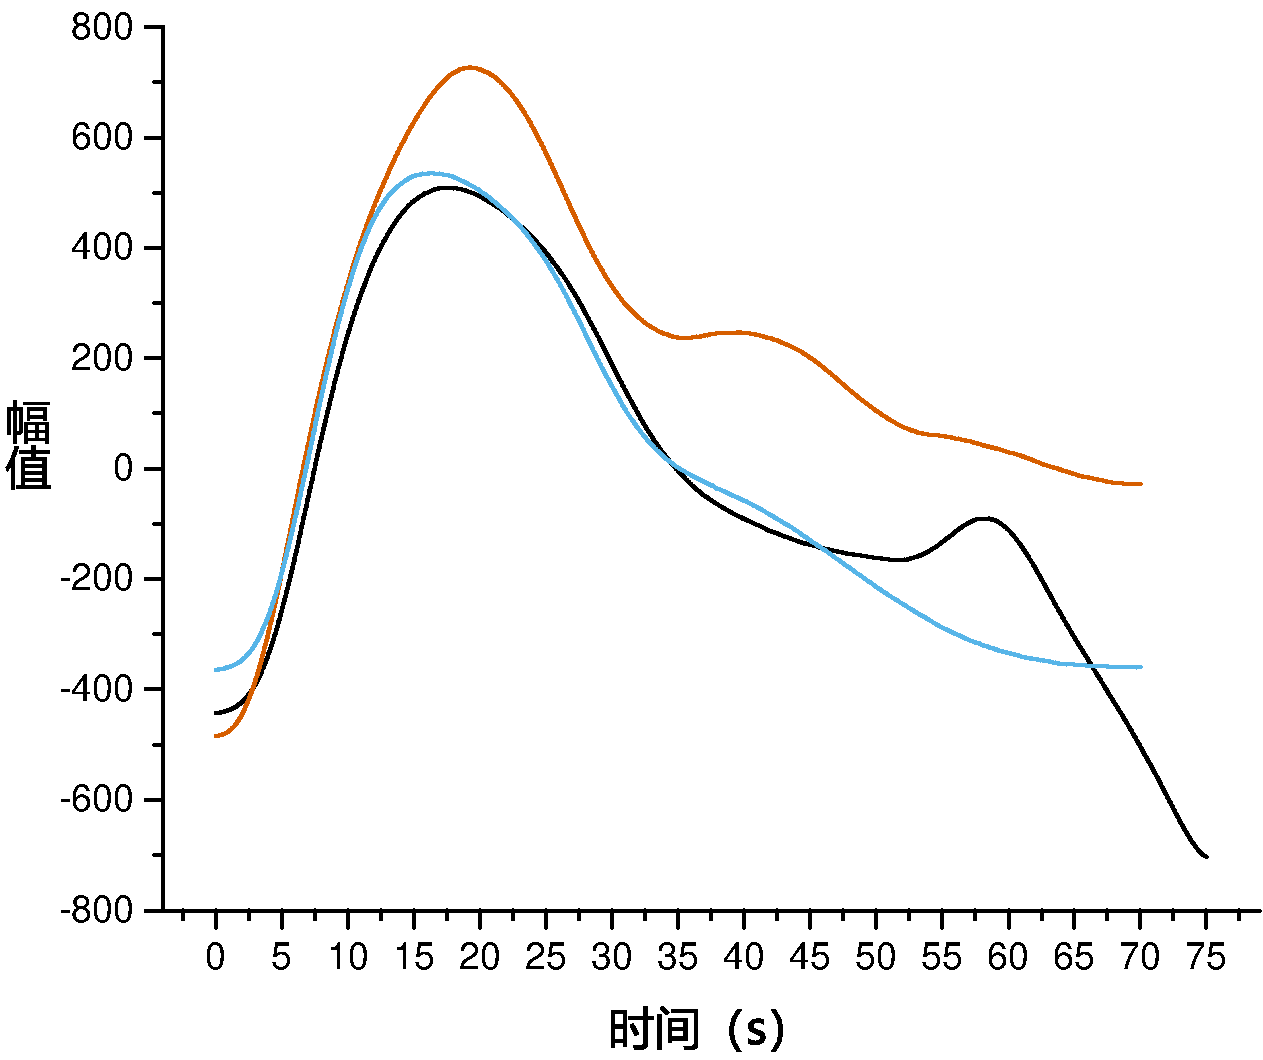
\includegraphics[width=.6\linewidth]{pulse_preprocess/pulsecontrast}
    \caption[同一名被试PPG信号三段波形对比]{\label{fig:pulsecontrast}同一名被试PPG信号三段波形对比。波形按起点时间对齐,此外无任何其他预处理操作。可以看到三段波形在重搏的显著程度、时长、幅值等方面均有所差异。}
\end{figure}
\subsection{时频特征的取舍}
通常而言,对生理信号进行分析可以采取时域-频域联合分析方法,分别从时域及频域提取相关特征进行参数描述及后续分析工作。
针对本研究而言,由于使用的是脉搏波信号,其频域带宽窄,且数据采集实验得到的数据已经在硬件采集设备上进行过频段选择,频率成分
构成相对简单,故不适用频域特征分析方法。此外,本实验得到的数据长度有限,单条数据长度约1-3分钟,因此,另一类常见的非线性参数特征参数的分析在此情况下也不适用。
故本研究主要仅从\textbf{时域角度}对脉搏波进行特征提取与描述工作。

\subsection{脉搏波时域特征}
本小节将前人提出的脉搏波时域特征进行了汇总整理,将PPG相关描述特征按计算时是否基于完整PPG波形分为基于波形与基于时间窗等两大类。其中,基于时间窗的特征又可进一步细分为基于5s、10s等固定窗长与不定窗长等两大类。
特别地,本小节也对已在子痫前期的相关研究中得到应用的脉搏波(含压力脉搏波)特征参数进行了详细说明。

一、基于波形的时域特征

在诸多PPG波形形态学特征参数中,时间类参数、幅度类参数与面积类参数往往定义清晰明了、意义明确易于理解、且易与脉搏波产生原理过程联系起来,从而具有一定的生理学意义。
因此,这些参数在基于PPG的各类研究中得到了最广泛的应用\cite{cwl,mmt}。除这三类参数外,斜率类参数也在描述脉搏波形态特征领域占有一席之地。
最后,在信号分析领域得到广泛使用的通用无量纲参数与高阶统计参数也可在一定程度上反应PPG信号特征。
以下是各类参数的具体介绍。

1. 时间类特征参数

时间类特征参数描述了PPG波形中某些特殊点之间的时长值或多个这样时长之间的比例关系。脉搏传导时间(Pulse Transit Time,PTT)则是其中最有代表性的时间类参数之一。
如\autoref{fig:ri}所示,PTT是对脉搏波主波峰与重博波波峰或反射波导致的拐点之间的时间间隔的量化描述\cite{Brumfield2005,Su2014}。PTT在基于PPG的各类研究中得到了广泛应用。
\begin{figure}[htbp]
    \centering
    \subfigure[\label{fig:ri1}重博波明显的PPG波形]{
    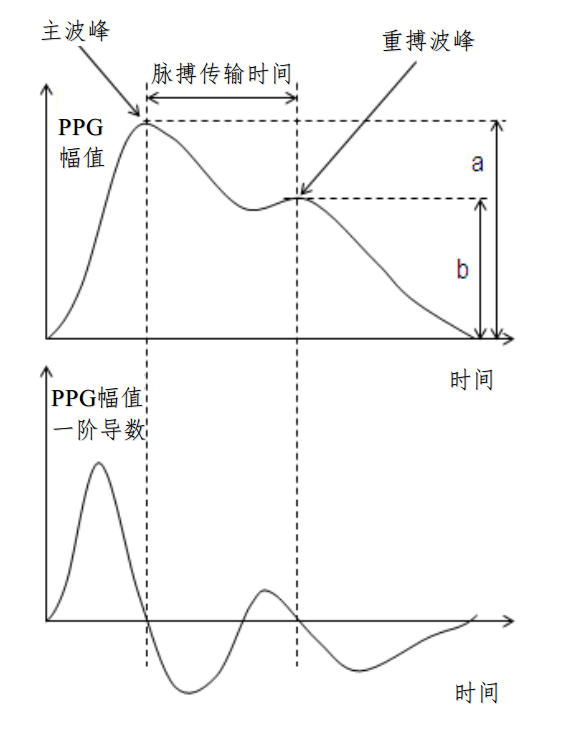
\includegraphics[width=5.5cm]{pulse_preprocess/ri1}
    }
    \quad
    \subfigure[\label{fig:ri2}重博波不明显的PPG波形]{
    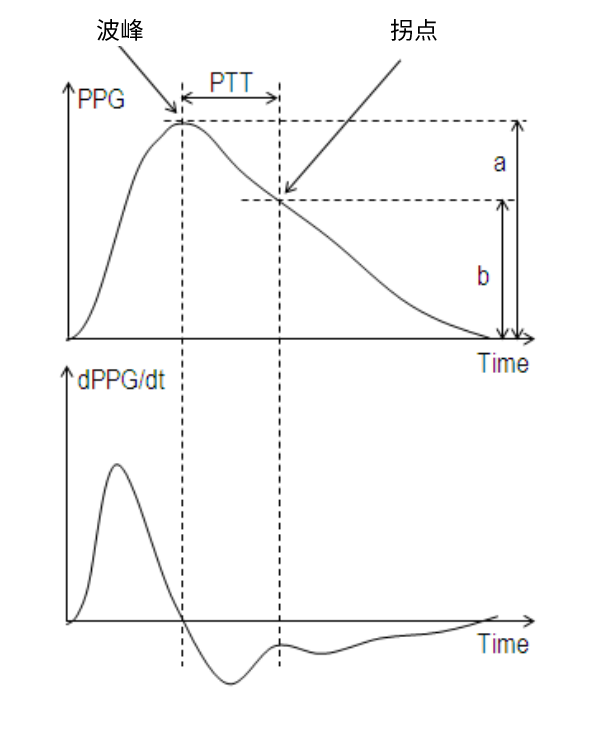
\includegraphics[width=5.5cm]{pulse_preprocess/ri2}
    }
    \caption[PTT及RI计算原理示意]{\label{fig:ri}PTT及RI计算原理示意\cite{Su2014}}
\end{figure}

除PTT外,时间类特征参数还包含脉搏波脉动周期、上升支间期、下降支间期等。2016年,王梦婷提出了一种描述动脉内高压力水平维持的时间参数,并在此基础上归一化处理后得到了多项衍生参数,
包含动脉高压力持续时间、血管硬度指数、心肌收缩系数及心博出系数等\cite{mmt}。
2018年,陈婉琳等人基于斜率极值提出了上升支最大斜率间期、下降支最小斜率间期等参数\cite{cwl}。以上参数的定义参见\autoref{fig:timefeature}及\autoref{tab:timefeature}所示。
\begin{figure}[htbp]
    \centering
    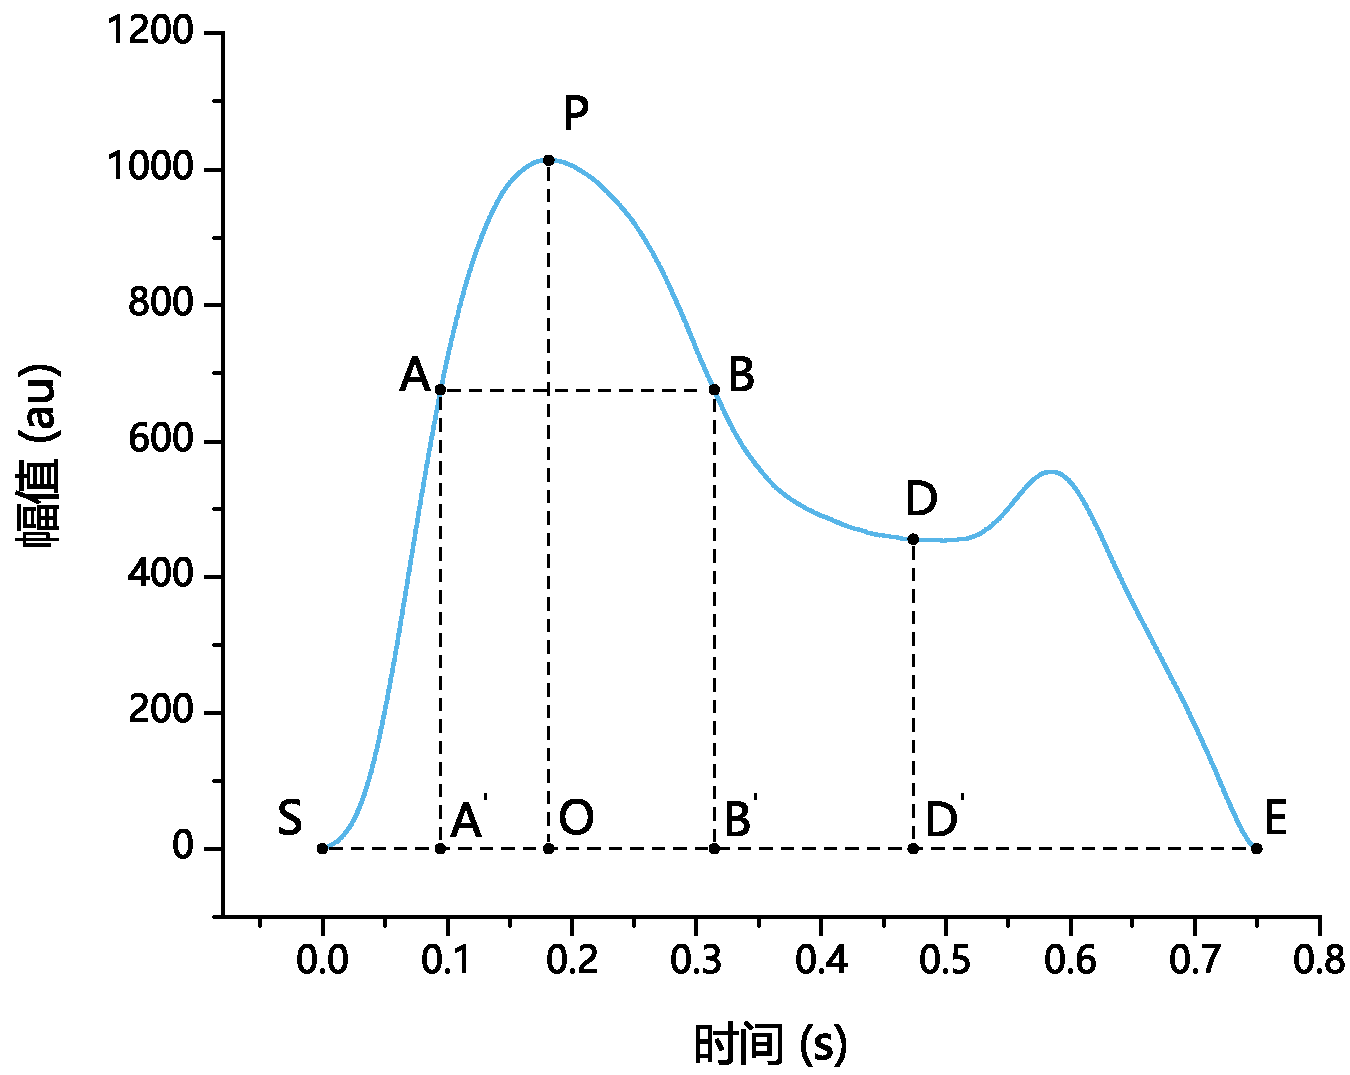
\includegraphics[width=.6\linewidth]{pulse_preprocess/timefeature}
    \caption[PPG时间及幅值类参数示意]{\label{fig:timefeature}PPG时间及幅值类参数示意。其中,AA'的幅值为主波峰值的2/3,D点为降中峡。}
\end{figure}
\begin{table}[h]
    \centering
    \zihao{-4}
    \caption{\label{tab:timefeature}常见PPG时间类参数定义}
    \begin{tabularx}{\linewidth}{cX<{\centering}c}
    \toprule
    \textbf{参数} & \textbf{物理意义} & \textbf{表达式} \\
    \midrule
    脉动周期      &  相邻两个波谷之间的时间间隔         &  $SE$\\
    上升支间期      &  从波形起点(波谷)至主波峰之间的时间间隔         &  $SO$\\
    下降支间期      &  从主波峰至波形终点(波谷)之间的时间间隔        &  $OE$\\
    动脉高压力持续时间    &  主波维持在峰值幅值2/3高度的时间间隔         &    $A'B'$   \\
    血管硬度指数    &  动脉高压力持续时间与脉动周期的比值         &   $\frac{A'B'}{SE}$    \\
    心肌收缩系数    &  上升支间期与脉动周期的比值         &  $\frac{SO}{SE}$    \\
    心搏出系数      &   从波峰至降中峡的时间间隔与脉动周期的比值       &   $\frac{OB'}{SE}$\\
    上升支最大斜率间期      &   上升支波谷与上升支斜率最大点之间的时间间隔      &   /    \\
    下降支最大斜率间期      &   下降支斜率最小点与下降支波谷之间的时间间隔      &    /  \\
    \bottomrule
    \end{tabularx}
\end{table}

2. 幅值类特征参数

幅值类特征参数描述了PPG波形中某个时刻的幅值高度或多个时刻幅值高度之间的比例关系。在各项研究中得到普遍应用的脉搏波增强指数(Augmentation Index,AIX)、反射指数(Reflection Index,RI)及K值等
均属于幅值类参数。

AIX指心脏收缩期早期与晚期拐点之间的差值与峰值之比,计算的关键需要先找到表征脉搏波反射波上升冲程(up-stroke)的拐点$P1$,如\autoref{fig:aix}所示\cite{Su2014}。
\begin{equation}
    \label{equ:aix}
    AIX = \pm \frac{\Delta P}{PP}
\end{equation}
特别地,\autoref{equ:character}中$\pm$的取值视拐点$P1$与峰值点的相对位置而定。当拐点在脉搏波波峰点左侧时,AIX符号取正,表示主波峰是经过叠加得到的,如图\autoref{fig:aix1}所示;反之,
当拐点在脉搏波波峰点右侧时,AIX符号取负,表明主波峰未得到“增强”,如图\autoref{fig:aix2}所示。
\begin{figure}[htbp]
    \centering
    \subfigure[\label{fig:aix1}拐点在波峰左侧]{
    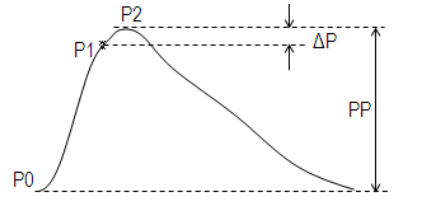
\includegraphics[width=5.5cm]{pulse_preprocess/aix1}
    }
    \quad
    \subfigure[\label{fig:aix2}拐点在波峰右侧]{
    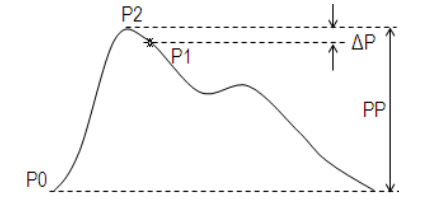
\includegraphics[width=5.5cm]{pulse_preprocess/aix2}
    }
    \caption[AIX计算原理示意]{\label{fig:aix}AIX计算原理示意\cite{Su2014}}
\end{figure}

RI是由脉搏波舒张峰值或拐点处幅值与收缩谷值之比计算得到的,如\autoref{fig:ri}所示\cite{Su2014,Elgendi2012}
\begin{equation}
    \label{equ:ri}
    RI = \frac{b}{a} \cdot 100\%
\end{equation}

K值是另一种在临床得到广泛应用的基于脉搏波面积变化的形态学特征无量纲参数,最早由罗志昌等人提出\cite{Luo1988,PPGYY}
\begin{equation}
    \label{equ:ppgk}
    K=\frac{P_m-P_d}{P_s-P_d}
\end{equation}
其中,$P_m=\frac{1}{T}\int_{0}^{T}P(t)dt$为一个心动周期内脉搏压力$P(t)$的平均值,$P_s$与$P_d$分别为收缩压与舒张压。罗志昌等人的研究表明,K值依赖于脉搏波的波形动态变化,
同时能够在很大程度上反应血管外周阻力与血管壁硬化程度等生理因素的变化。
\begin{figure}[htbp]
    \centering
    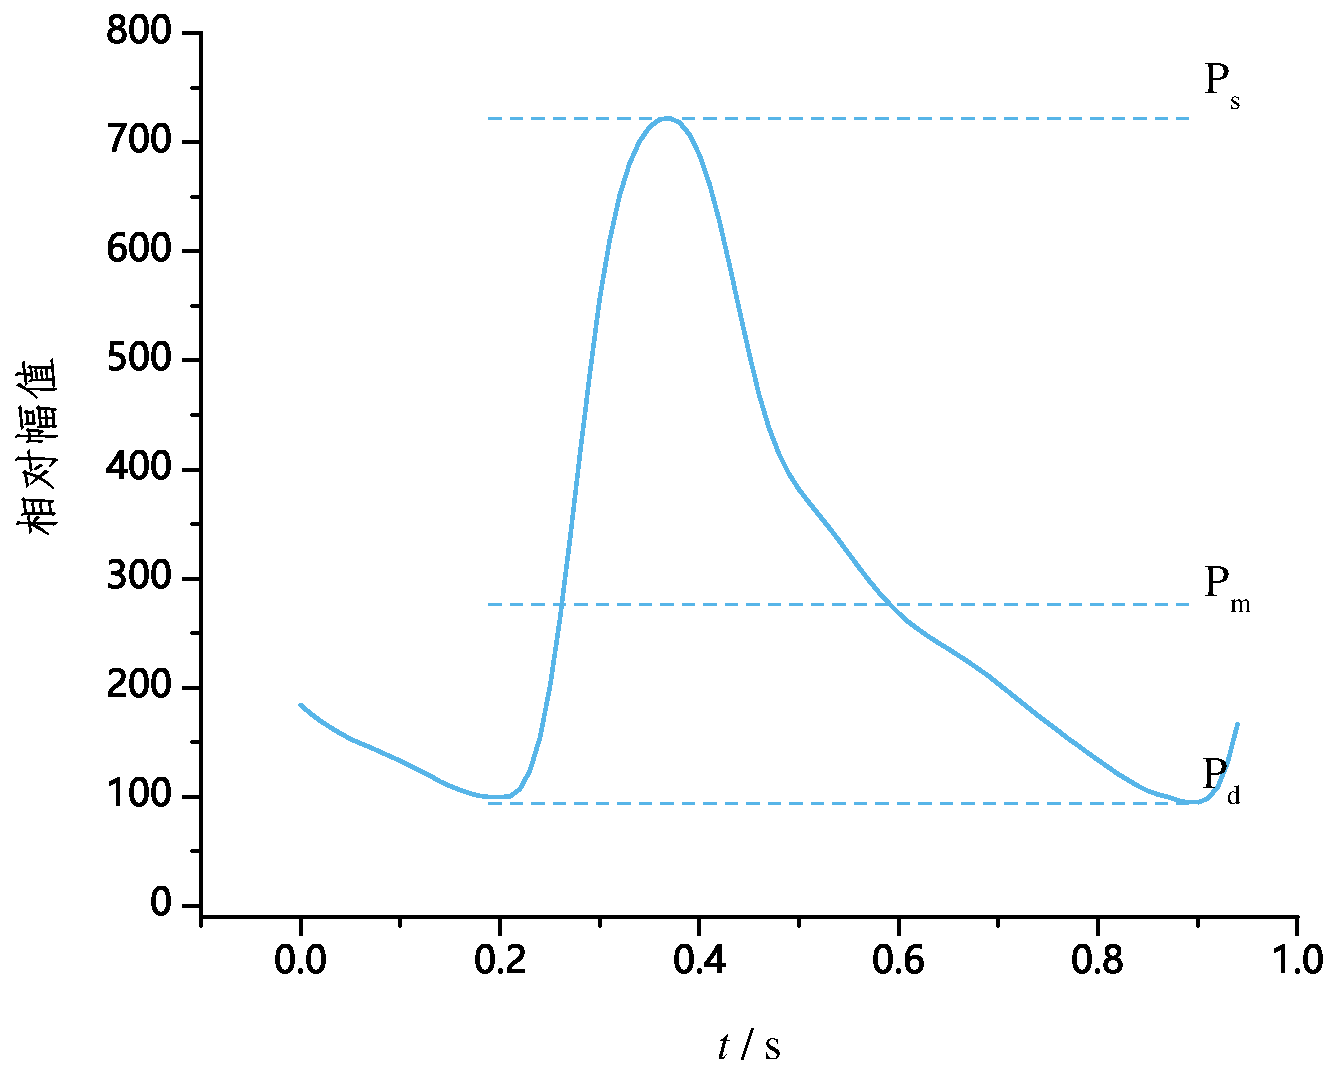
\includegraphics[width=.55\linewidth]{pulse_preprocess/k}
    \caption{\label{fig:k}K值的计算原理示意}
\end{figure}

除上述参数外,幅值类特征参数还包括脉搏波波峰幅值、波谷幅值差值、降中峡幅值及外周阻力系数等\cite{cwl,mmt}。这些参数的具体定义参见\autoref{fig:timefeature}及\autoref{tab:heightfeature}所示。
\begin{table}[htbp]
    \centering
    \zihao{-4}
    \caption{\label{tab:heightfeature}常见PPG幅值类参数定义}
    \begin{tabularx}{\linewidth}{cX<{\centering}c}
    \toprule
    \textbf{参数} & \textbf{物理意义} & \textbf{表达式} \\
    \midrule
    波峰幅值      &  主波峰幅值         &  $OP$\\
    波谷幅值差值      &  相邻波谷之间的幅值之差         &  /\\
    降中峡幅值      &  降中峡至基线幅值         &  $DD'$\\
    外周阻力系数      &  降中峡幅值与主波峰幅值之比         &  $\frac{DD'}{OP}$\\
    \bottomrule
    \end{tabularx}
\end{table}

3. 面积类特征参数

面积类参数计算依赖与脉搏波波形与基线所形成的面积,主要通过按时间方向对PPG波形曲线积分完成计算过程。
面积类参数可以看成是血管在一段时间内的血液容积的映射。
王梦婷在其研究中指出\cite{mmt},PPG上升支主要受心脏射血量与血压脉动影响,下降支主要受外周阻力影响。其中,上升支随心脏射血量增加愈益陡峭,射血时间越短,
其形态图像越向左上方凸出;而当外周阻力增加时,会导致动脉血管壁弹性下降,下降支波形向上方凸出。

常见的面积类特征参数包括上升支面积、下降支面积、
全周期面积、上升支面积比、下降支面积比、全周期面积比及(下降支)面积差值比(Area Difference Ratio,ADR)\cite{Feng2018}等。
以上参数的具体定义参见\autoref{tab:areafeature}及\autoref{fig:areafeature}。
\begin{center}
    \zihao{-4}
	\begin{longtable}{m{3.5cm}<{\centering}m{6.5cm}<{\centering}m{4.5cm}<{\centering}}
		\caption{PPG面积类参数示意}\\
		\label{tab:areafeature}\\
        \toprule
        \textbf{参数} & \textbf{物理意义} & \textbf{表达式} \\
        \midrule
        \endfirsthead
        \caption[]{(续)}\\
        \toprule
        \textbf{参数} & \textbf{物理意义} & \textbf{表达式} \\
        \midrule
        \endhead 
        \midrule
        \endfoot
        \bottomrule
        \endlastfoot
        上升支面积      &  从波形起点至峰值点对波形曲线积分所得面积值         &  $S_r=\int_{T_S}^{T_P}P(t)dt$\\
        下降支面积      &  从波形峰值点至终点对波形曲线积分所得面积值         &  $S_f=\int_{T_P}^{T_E}P(t)dt$\\
        全周期面积      &  脉搏波波形在一个完整周期内的积分所得面积值         &  $S_t=\int_{T_S}^{T_E}P(t)dt$\\
        上升支面积比    &  上升支面积与$\triangle OPS$面积之比         &   $R_r=\frac{S_r}{S_{\triangle OPS}}$    \\
        下降支面积比    &  下降支面积与$\triangle OPE$面积之比        &   $R_f=\frac{S_f}{S_{\triangle OPE}}$    \\
        全周期面积比    &  全周期面积与$\triangle SPE$面积之比         &   $R_t=\frac{S_t}{S_{\triangle SPE}}$    \\
        下降支面积差值比&  下降支面积和$\triangle OPE$面积之差与$\triangle OPE$面积之比        &    $\Delta R_f=\frac{S_{\triangle OPE}-S_f}{S_{\triangle OPE}}=1-R_f$\\
	\end{longtable}
\end{center}

\clearpage
\begin{figure}[htbp]
    \centering
    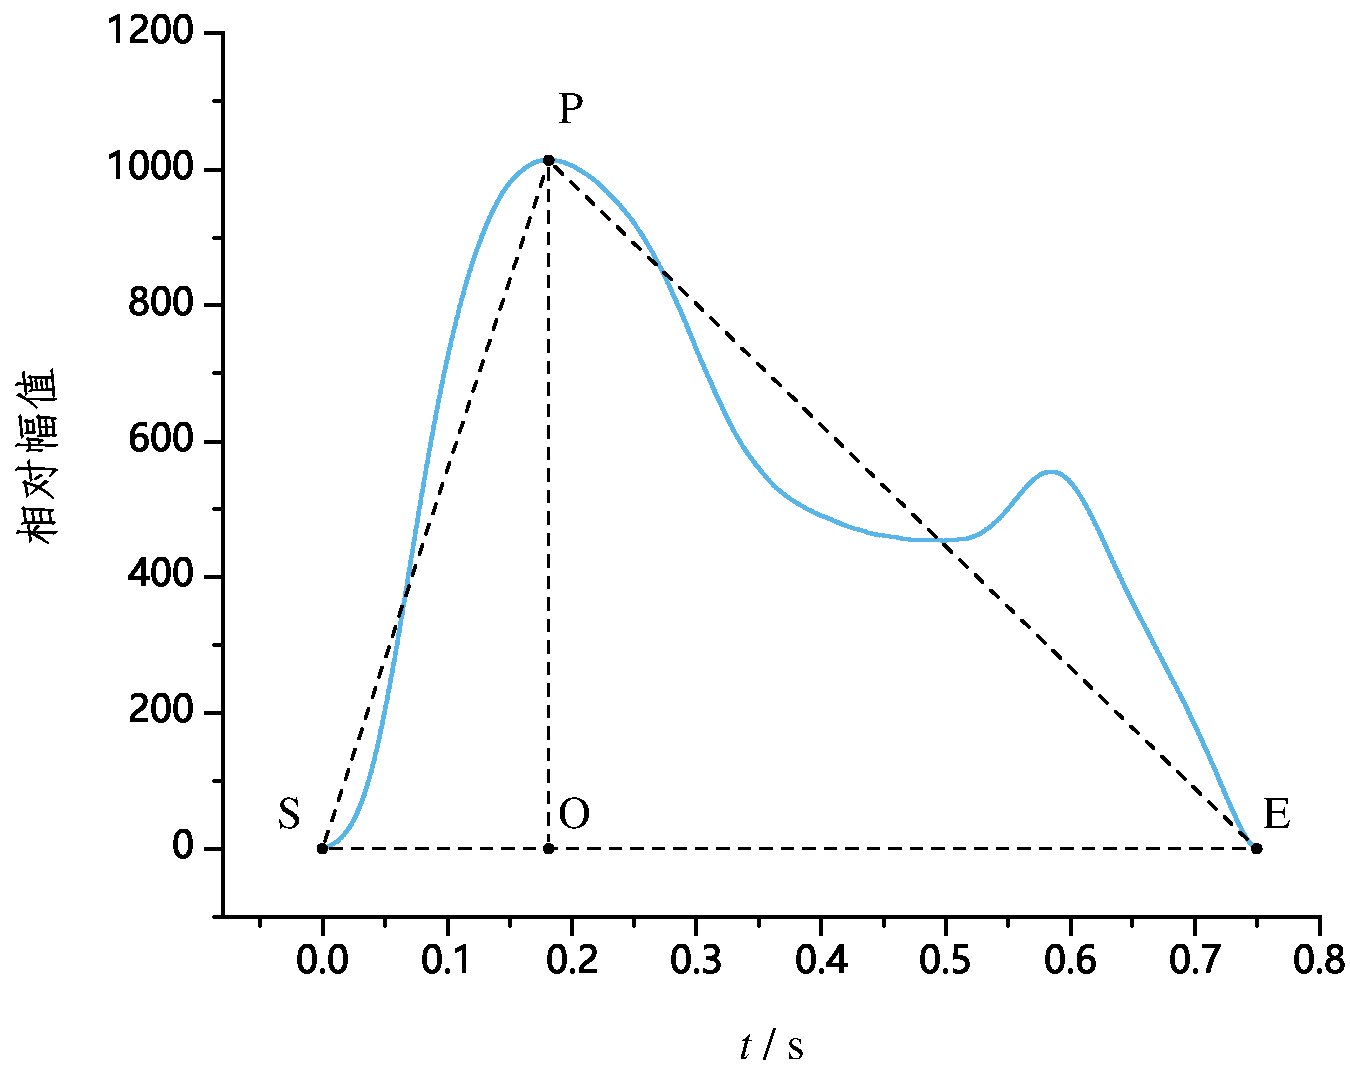
\includegraphics[width=.6\linewidth]{pulse_preprocess/areafeature}
    \caption{\label{fig:areafeature}PPG面积及斜率类参数示意}
\end{figure}

值得一提的是,Feng等人已经将ADR应用于子痫前期的研究中,其研究结果显示患有PE的孕妇与正常孕妇在PPG信号的ADR参数上具有统计意义上的显著差异(0.752 VS 0.723,P<0.01)\cite{Feng2018}。

另外需要注意的是,从\autoref{tab:areafeature}中的参数定义不难发现,ADR与下降支面积比完全线形相关,两者之间满足
\begin{equation}
    \label{equ:adr}
    ADR = 1-R_f
\end{equation}
此外,王选在其研究中也证明了全周期面积比与幅值类参数K值完全线性相关\cite{Wang2012}
\begin{equation}
    \label{equ:kandart}
    R_t=\frac{S_t}{S_{\triangle SPE}}=\frac{\int_{0}^{T}P(t)dt}{\frac{1}{2}P_sT}=\frac{2\cdot P_mT}{P_sT}=2\cdot K
\end{equation}
因此,若需要使用这两组参数对PPG进行描述时,只需视情况分别从每组中选取一个即可。

4. 斜率类特征参数

斜率类参数是对PPG波形在一段时间内幅值的上升/下降速率的快慢的量化描述,反应了血液容积在这段时间内的平均流速。

光电容积斜率指数(photoplethysmography slope index,PSI)是斜率类参数中比较有代表性的一种\cite{Chen2019}。其计算的基本思想是将PPG波形分段后再描述各段之间的幅值变化,
如\autoref{fig:psi}所示。值得一提的是,陈婉琳等人的研究发现PSI可以在一定程度上对PE患者进行识别\cite{Chen2019}。
\begin{figure}[htbp]
    \centering
    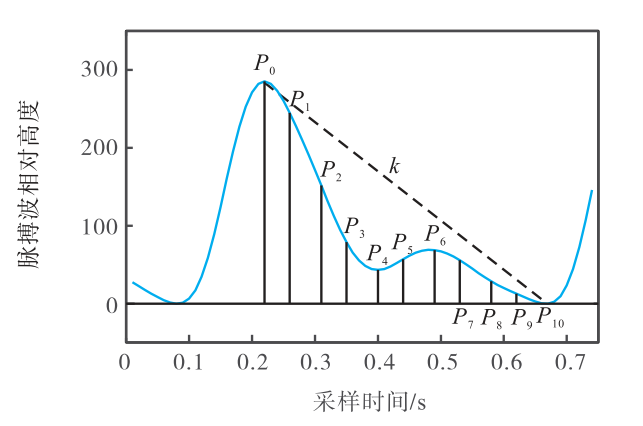
\includegraphics[width=.6\linewidth]{pulse_preprocess/psi}
    \caption[PSI计算原理示意]{\label{fig:psi}PSI计算原理示意\cite{Chen2019}}
\end{figure}

此外,常见的斜率参数还包括上升支平均斜率、上升支最大斜率、下降支平均斜率、下降支最大斜率等。这些参数的具体定义参见\autoref{fig:areafeature}及\autoref{tab:slopefeature}所示。
\begin{table}[htbp]
    \centering
    \zihao{-4}
    \caption{\label{tab:slopefeature}常见PPG斜率类参数定义}
    \begin{tabularx}{\linewidth}{cX<{\centering}c}
    \toprule
    \textbf{参数} & \textbf{物理意义} & \textbf{表达式} \\
    \midrule
    上升支平均斜率      &  主波峰值与上升支时间之比         &  $\frac{OP}{SO}$\\
    下降支平均斜率      &  主波峰值与下降支时间之比         &  $-\frac{OP}{OE}$\\
    上升支最大斜率      &           &  /\\
    下降支最小斜率      &           &   /    \\
    \bottomrule
    \end{tabularx}
\end{table}

二、其他特征

除上述特征参数外,在PPG的其他研究领域还有一些较为知名的特征参数,大动脉僵硬指数(stiffness index,SI)与脉搏波波形速度(Pulse Wave Velocity,PWV)就是其中最为典型的代表。

SI被定义为是被试身高$h$与脉搏波的主波峰值降中峡的时间间隔$\Delta T$的比值\cite{Elgendi2012,Millasseau2002,Brumfield2005},即
\begin{equation}
    \label{equ:si}
    SI = \frac{h}{\Delta T}
\end{equation}
Millasseau等人的研究表明随着大动脉硬度增加、主动脉和大动脉中压力波的脉搏波速度增加,
收缩和舒张峰值之间的时间延迟也会随着年龄的增长而减少,导致SI也会随着年龄增长而增长,如\autoref{fig:si}所示\cite{Elgendi2012,Millasseau2002,Brumfield2005}。
\begin{figure}[htbp]
    \centering
    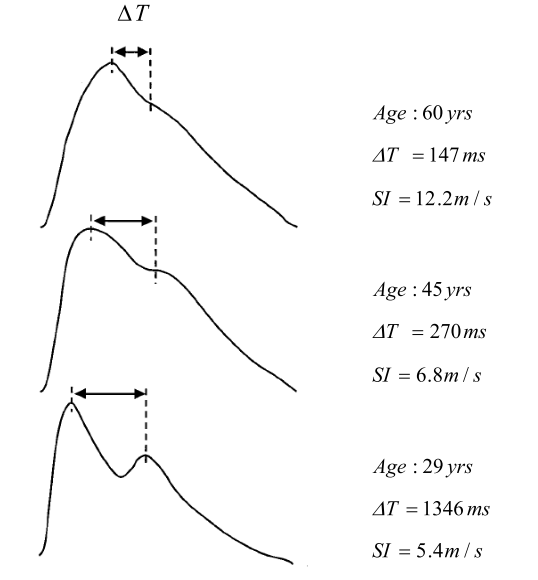
\includegraphics[width=.4\linewidth]{pulse_preprocess/si}
    \caption[SI计算原理示意]{\label{fig:si}SI计算原理示意\cite{Elgendi2012,Millasseau2002,Brumfield2005}}
\end{figure}

脉搏波波形速度(Pulse Wave Velocity,PWV)是指心脏每次搏动射血产生的沿大动脉壁传播的压力波传导速度\cite{Van2012}。在计算PWV时,需要在人体两部位分别测量脉搏波信号。
若记两测量部位的直线距离的80\%为$d$,两部位之间的脉搏波传导时间差为$t$,则有
\begin{equation}
    \label{equ:pwv}
    PWV = \frac{d}{t}
\end{equation}
PWV已被证实与动脉扩张性、僵硬度、管壁厚度和血液黏稠度密切相关。
特别地,PWV已经在子痫前期的诸多研究中得到应用\cite{Tomsin2012,Katsipi2014,VivianaIvan2018,Ira2014}。
需要注意的是,由于PWV的测量依赖于在人体不同部位测量脉搏波(且测量多利用压力传感器完成),故\textbf{不适用}单点测量的光电容积脉搏波研究。

\subsection{基于波形的新型时域特征参数设计}
在总结前人研究基础上,本研究结合脉搏波形态特点,设计了多种新型时域描述参数,以求从新的角度完成对脉搏波波形特征的描述。

一、波形特征的设计基础

以纯数学的角度来看,PPG的信号波形可以近似描述为从一条往复于水平基线与波峰之间的双向路径。一般而言,由于PPG信号的上升支通常较下降支更为简单,该双向路径可以进一步简化为从波峰下降至水平基线的一条单向路径,只要完成对该单向路径的描述
即可类比完成上升支的描述,从而完成对整个脉搏波波形的描述,如\autoref{fig:road}所示。
\begin{figure}[htbp]
    \centering
    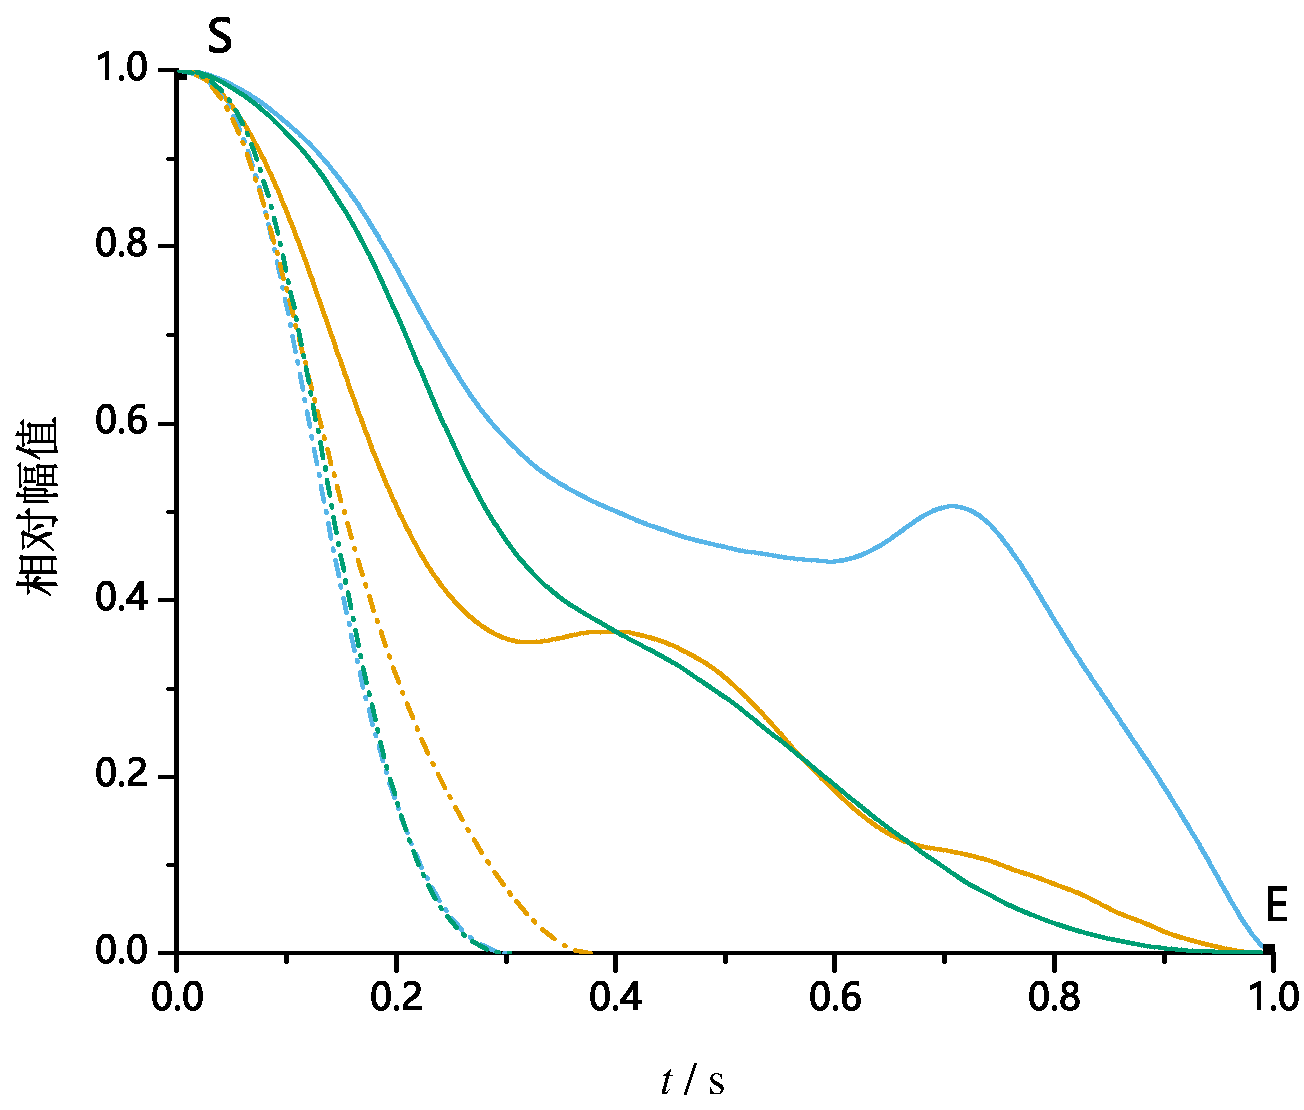
\includegraphics[width=.6\linewidth]{pulse_preprocess/road}
    \caption[脉搏波波形的单向路径表示]{\label{fig:road}脉搏波波形的单向路径表示。其中三条路径由\autoref{fig:pulsecontrast}所示的同一被试的三段波形对应线形变换得来。同一颜色的实线部分与虚线部分对应同一个脉搏波的下降支与上升支
    ,其中,下降支按一定比例缩放至目标区间内,上升支水平反向按同一比例反向进行了缩放。}
\end{figure}

由信号的采样定理可知,对上述路径的描述可通过对路径上一系列点的描述来完成。不失一般性,若将下降支的单向路径的起点坐标与终点坐标分别设置为S$(0,1)$与E$(1,0)$。
对于该路径上任意一点P,可以用原点O坐标$(0,0)$与路径始末点坐标S、E等为基本参照点,以及P
在X轴、Y轴上的投射点$P_x$、$P_y$等衍生参照点进行对该点进行描述,如\autoref{fig:point}所示。
此时对P点进行描述可使用\autoref{tab:pointsdesc}中的定义参数指标,部分参数指标的归一化/类归一化无量纲形式也在表中进行了说明。
% 同一类型下关于起始S、E两点对偶的参数只保留了一个。
\begin{figure}[htbp]
    \centering
    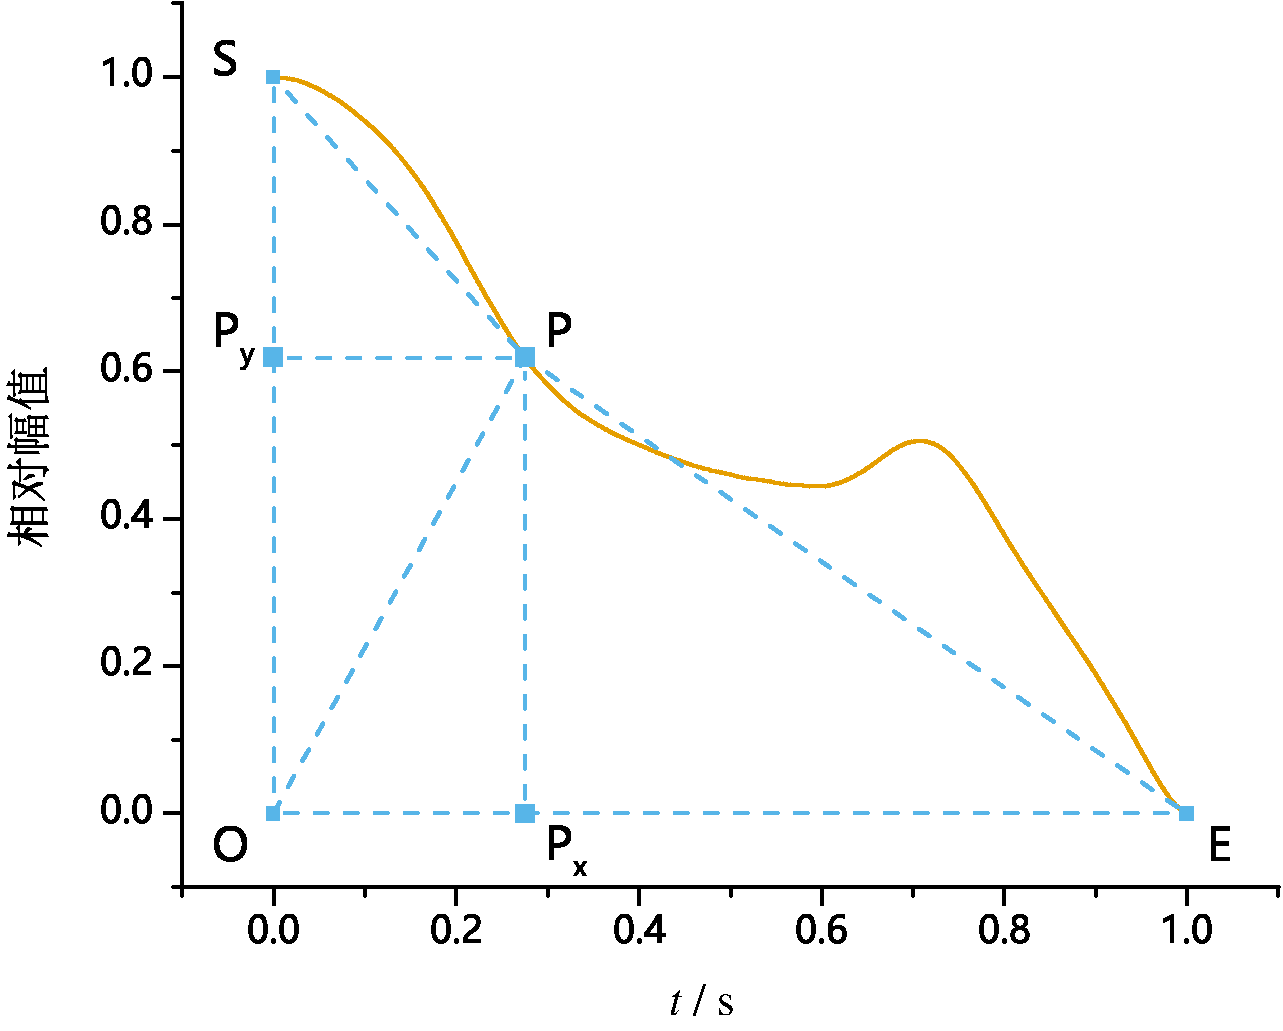
\includegraphics[width=.6\linewidth]{pulse_preprocess/point}
    \caption{\label{fig:point}单向路径上点的描述}
\end{figure}
\begin{center}
    \zihao{-4}
    % Plan A
    % \setlength\LTleft{0pt}
    % \setlength\LTright{0pt}
	% \begin{longtable}{@{\extracolsep{\fill}}|c|c|c|c|c|}
    % Plan B
    % m表示居中,p为置顶,b为置底
    % 列宽总计16cm,各列按需分配长度,p{x-0.43cm}<{\centering}即可
    % \begin{longtable}{p{1.6cm}<{\centering}p{4.1cm}<{\centering}p{2.1cm}<{\centering}p{4.1cm}<{\centering}p{2.1cm}<{\centering}}
    \begin{longtable}{m{1.57cm}<{\centering}m{4.07cm}<{\centering}m{2.07cm}<{\centering}m{4.07cm}<{\centering}m{2.07cm}<{\centering}}
		\caption{单向路径上任意一点的描述指标一览}\\
		\label{tab:pointsdesc}\\
		\hline\hline
        \multirow{2}[2]{*}{\textbf{参数类型}} & \multicolumn{2}{c}{\textbf{原始数值表达}} & \multicolumn{2}{c}{\textbf{归一化表达}} \\
            & \multicolumn{1}{c}{物理意义} & \multicolumn{1}{c}{表达式或公式} & \multicolumn{1}{c}{物理意义} & \multicolumn{1}{c}{表达式或公式} \\
        \hline
        \endfirsthead
        \caption[]{(续)}\\
        \hline
        \multirow{2}[2]{*}{\textbf{参数类型}} & \multicolumn{2}{c}{\textbf{原始数值表达}} & \multicolumn{2}{c}{\textbf{归一化表达}} \\
            & \multicolumn{1}{c}{物理意义} & \multicolumn{1}{c}{表达式或公式} & \multicolumn{1}{c}{物理意义} & \multicolumn{1}{c}{表达式或公式} \\
        \hline
        \endhead 
        \hline
        \endfoot
        \hline\hline
        \endlastfoot
                                    & Y轴方向下降高度           &   $SP_y$      &  Y轴方向下降比例     & $\frac{SP_y}{OS}$ \\
                                    & P点高度                  &   $OP_y$       &    P点高度与波峰比值   & $\frac{OP_y}{OS}$ \\
                                    & 从S点到P点所用时间        &    $OP_x$   &      起点至P点所用时间与下降支总时长比值 & $\frac{OP_x}{OE}$ \\
                                    & 从P点到E点所用时间        &    $EP_x$   &      P点至终点E所用时间与下降支总时长比值 & $\frac{EP_x}{OE}$ \\
                                    & OP两点间几何距离        &    $OP$   &  OP两点距离与SE两点距离之比     & $\frac{OP}{SE}$ \\
                                    & SP两点间几何距离        &    $SP$   &  SP两点距离与SE两点距离之比     & $\frac{SP}{SE}$ \\
        \multirow{-7}*{线段}         & PE两点间几何距离        &    $PE$   &  PE两点距离与SE两点距离之比     & $\frac{PE}{SE}$ \\
                                    &  SP两点间曲线弧长     &  $L_{\overset{\frown}{SP}}$     &     SP两点间曲线弧长与SE两点直线距离之比  & $\frac{L_{\overset{\frown}{SP}}}{SE}$ \\
        \multirow{-2}*{曲线长度} &  PE两点间曲线弧长   &   $L_{\overset{\frown}{PE}}$    &    PE两点间曲线弧长与SE两点直线距离之比  &  $\frac{L_{\overset{\frown}{PE}}}{SE}$\\
                                    &  线段SP的斜率     &  $-\frac{SP_y}{PP_y}$     &   /    &  /  \\
                                    &  线段PE的斜率     &   $-\frac{P_yP_x}{EP_x}$    &    /  &  /   \\
        \multirow{-3}*{斜率}        &  线段OP的斜率    &    $\frac{PP_y}{PP_x}$   &    /   &  /     \\
                                    &  $\angle SPP_y$的弧度      & $\arctan(\frac{SP_y}{PP_y})$     &    /  &  /   \\
                                    &   $\angle POE$的弧度    &  $\arctan(\frac{P_yP_x}{EP_x})$      &    /  &  /   \\
        \multirow{-3}*{弧度(角度)}&   $\angle PEO$的弧度   &  $\arctan(\frac{PP_y}{PP_x})$         &    /  &  /   \\
                                    &    坐标轴、曲线与$PP_y$以上围成的面积   &  $\int_{P_y}^{S}{P(t)dy} $     &   前述面积与整体面积之比    & $\frac{\int_{P_y}^{S}{P(t)dy}}{\int_O^E{P(t)dx}}$ \\
                                    &   坐标轴、曲线与$OP$以左围成的面积   &    $\int_{O}^{P_x}{P(t)dx}-S_{\triangle OPP_x}$   &  前述面积与整体面积之比     & $\frac{\int_{O}^{P_x}{P(t)dx}-S_{\triangle OPP_x}}{\int_O^E{P(t)dx}}$ \\
                                    &   坐标轴、曲线与$PP_x$以左围成的面积   &   $\int_{O}^{P_x}{P(t)dx}$    &  前述面积与整体面积之比     & $\frac{\int_{O}^{P_x}{P(t)dx}}{\int_O^E{P(t)dx}}$ \\
        \multirow{-4}*{面积}        &    曲线与$SP$围成的面积   &   $\int_{P_y}^{S}{P(t)dy}-S_{\triangle SPP_y} $    &   /    &  /\\
	\end{longtable}
\end{center}

结合\autoref{tab:pointsdesc}与\autoref{fig:point}不难发现,只要在描述路径上任意确定一点$P$,与$P$关联的线段指标、曲线长度指标、斜率指标、弧度指标及面积指标等都可以得到确定并有与之对应的唯一数值。
反之,若以\autoref{tab:pointsdesc}中某一指标为基准,并在该指标的值域内选定一具体数值,则在描述路径上也可以确定与之对应的参考点$P'$,进一步可由$P'$得到其他描述参数的具体数值。
前文介绍的诸多学者的在各项研究中提出的PPG描述参数均不外乎是这样的过程。

二、脉搏波波形特征描述向量

本研究提出的脉搏波波形特征描述向量(Photoplethysmographic pulse feature vector,PPFV)是对一类量化PPG波形形态特点特征参数的统称。
与前文介绍的诸多仅用一个数值来表征PPG的参数不同,PPFV最显著的特点在于其用一组相互联系的数值来完成对PPG波形的量化描述
\begin{equation}
    \label{equ:featurevector}
    \boldsymbol {V_n}=[v_0,v_1,\cdots,v_{n-1}]
\end{equation}
其中,$n$是特征描述向量的维数,可以视情况人工设定。在本研究中,$n$的取值一般在[8,10]。

若设定原始信号某一PPG波形的采样点数为$N$,则该原始采样数据可以视为$n=N$的特殊PPFV;同理,当该波形经插值处理后的数据可以看成$n>N$的超维PPFV;
最后,使用此前介绍的各类时域参数对波形进行描述时,这些参数可视为$n=1$的特殊PPFV。
显然,在这一过程中可以发现,PPFV对波形的描述能力随着其向量维数的增加而增强,与之相反的,对波形的抽象与概括能力在此过程中则是削弱的。
这一现象可以用信息论中的编码理论进行解释,即通讯过程中在信源原始符号不变的情况下,
增加变换编码的输出符号长度可以提高系统的信息传输能力\cite{Zhao2017}。
从这个角度理解,PPFV是在变换编码背景下一种编码长度与信息描述能力的折中与妥协。

另一方面,PPFV的定义中存在着用来描述的数值需要有相互联系的限制。这里的相互联系可以理解为按照一定的规则在脉搏波上选取$n$个数据点,并从上小节波形特征的设计基础概括的\autoref{tab:pointsdesc}中
选取同一个参数完成n个具体数值的计算,即可得到一个实例化的$n$维向量PPFV。其中的规则是指对这$n$个点的采样方式,可从线段、曲线长度、斜率、弧度及面积等方面均匀或非均匀采样完成。

三、面积类特征参数的优化

重新考察\autoref{fig:areafeature}、\autoref{tab:areafeature}与\autoref{fig:point}、\autoref{tab:pointsdesc}中所示的各种面积类参数可以发现,这类面积类特征的计算过程多数涉及到累加积分运算,会不可避免地导致
PPG波形的细节信息无法在最终的数值中得到体现
\begin{equation}
    \label{equ:area1}
    S = \int_{t_0}^{t_n}P(t)dt \approx \frac{\Delta t}{2} \sum_{i=0}^{n-1}{(P(i)+P(i+1))}
\end{equation}
换言之,我们无法仅从面积类参数的数值上反推其原始波形的细节特征。两个在形态上迥异的PPG波形可能在某一面积类参数上具有相同数值。
为弥补此类面积参数对细节描述的不足,一种最直接的思路是使用\autoref{equ:area1}计算数值时,给予每个累加项一定的权值,即
\begin{equation}
    \label{equ:area2}
    S \approx \frac{\Delta t}{2} \sum_{i=0}^{n-1}{k_{i} (P(i)+P(i+1))}
\end{equation}
其中,加权系数$k_{i}$必须要进行一定的设计,需要能在反映细节的同时也降低权值本身的影响。
\begin{figure}[h]
    \centering
    \subfigure[\label{fig:pow}幂函数簇在0<x<1区间内图像。]{
    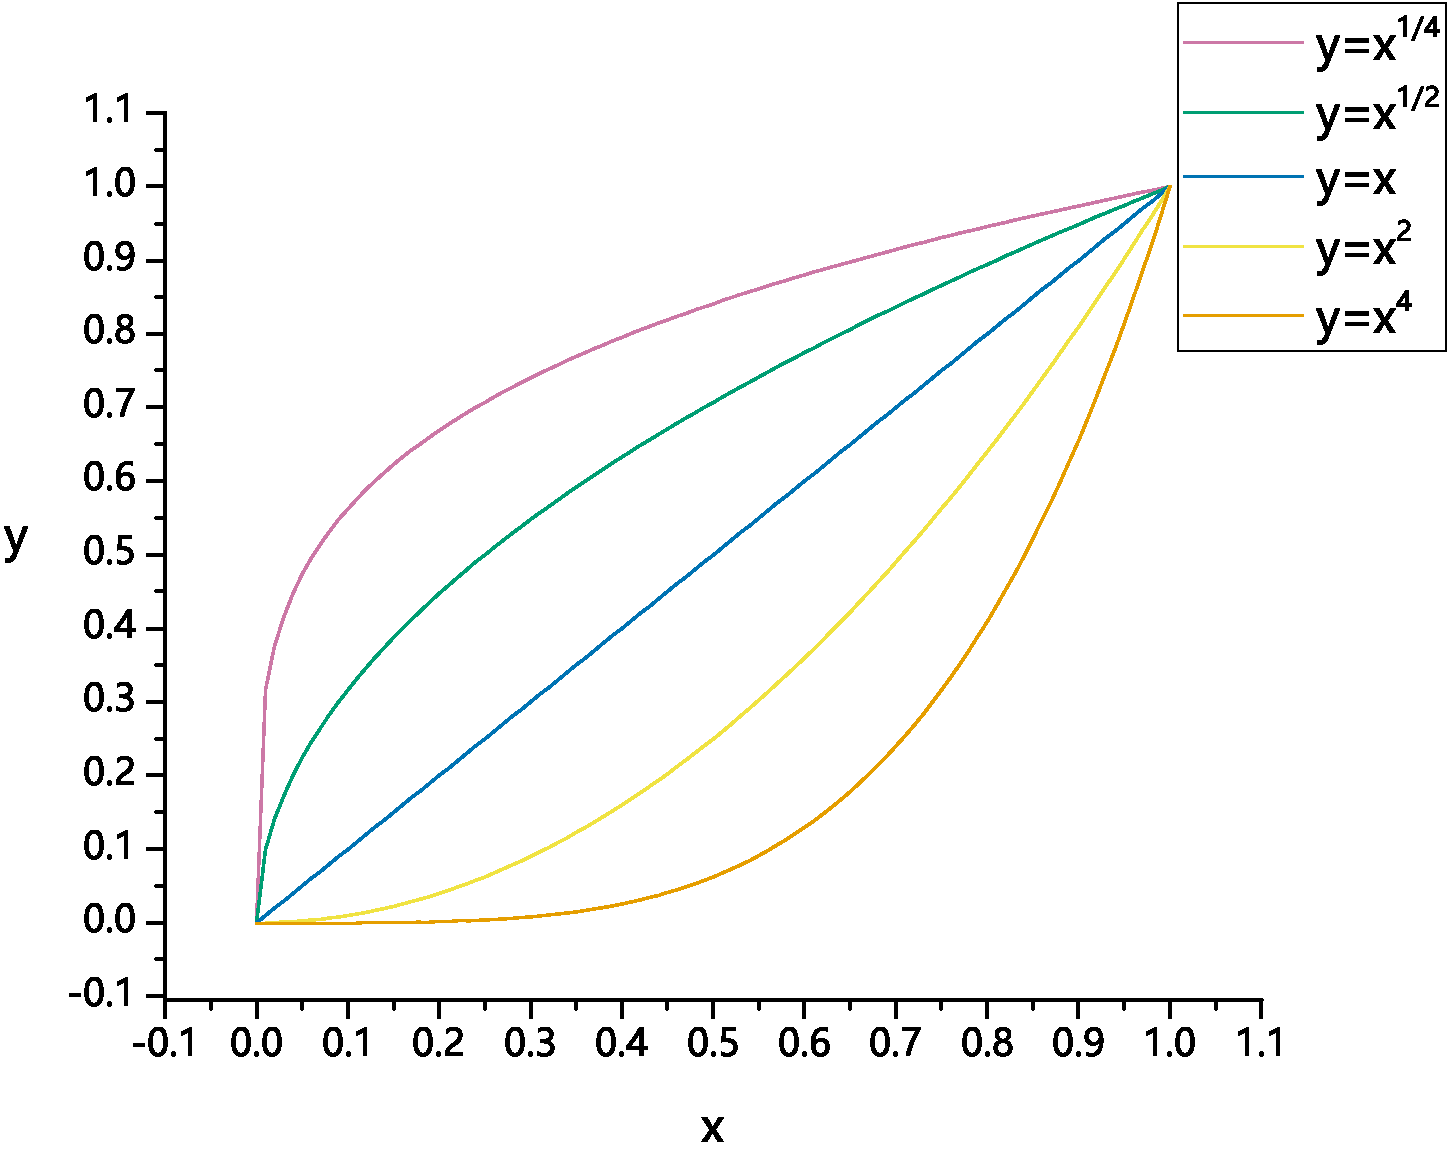
\includegraphics[width=5.5cm]{pulse_preprocess/pow}
    }
    \quad
    \subfigure[\label{fig:edi1}对\autoref{fig:pulsecontrast}中脉搏波波形进行EDI计算 I]{
    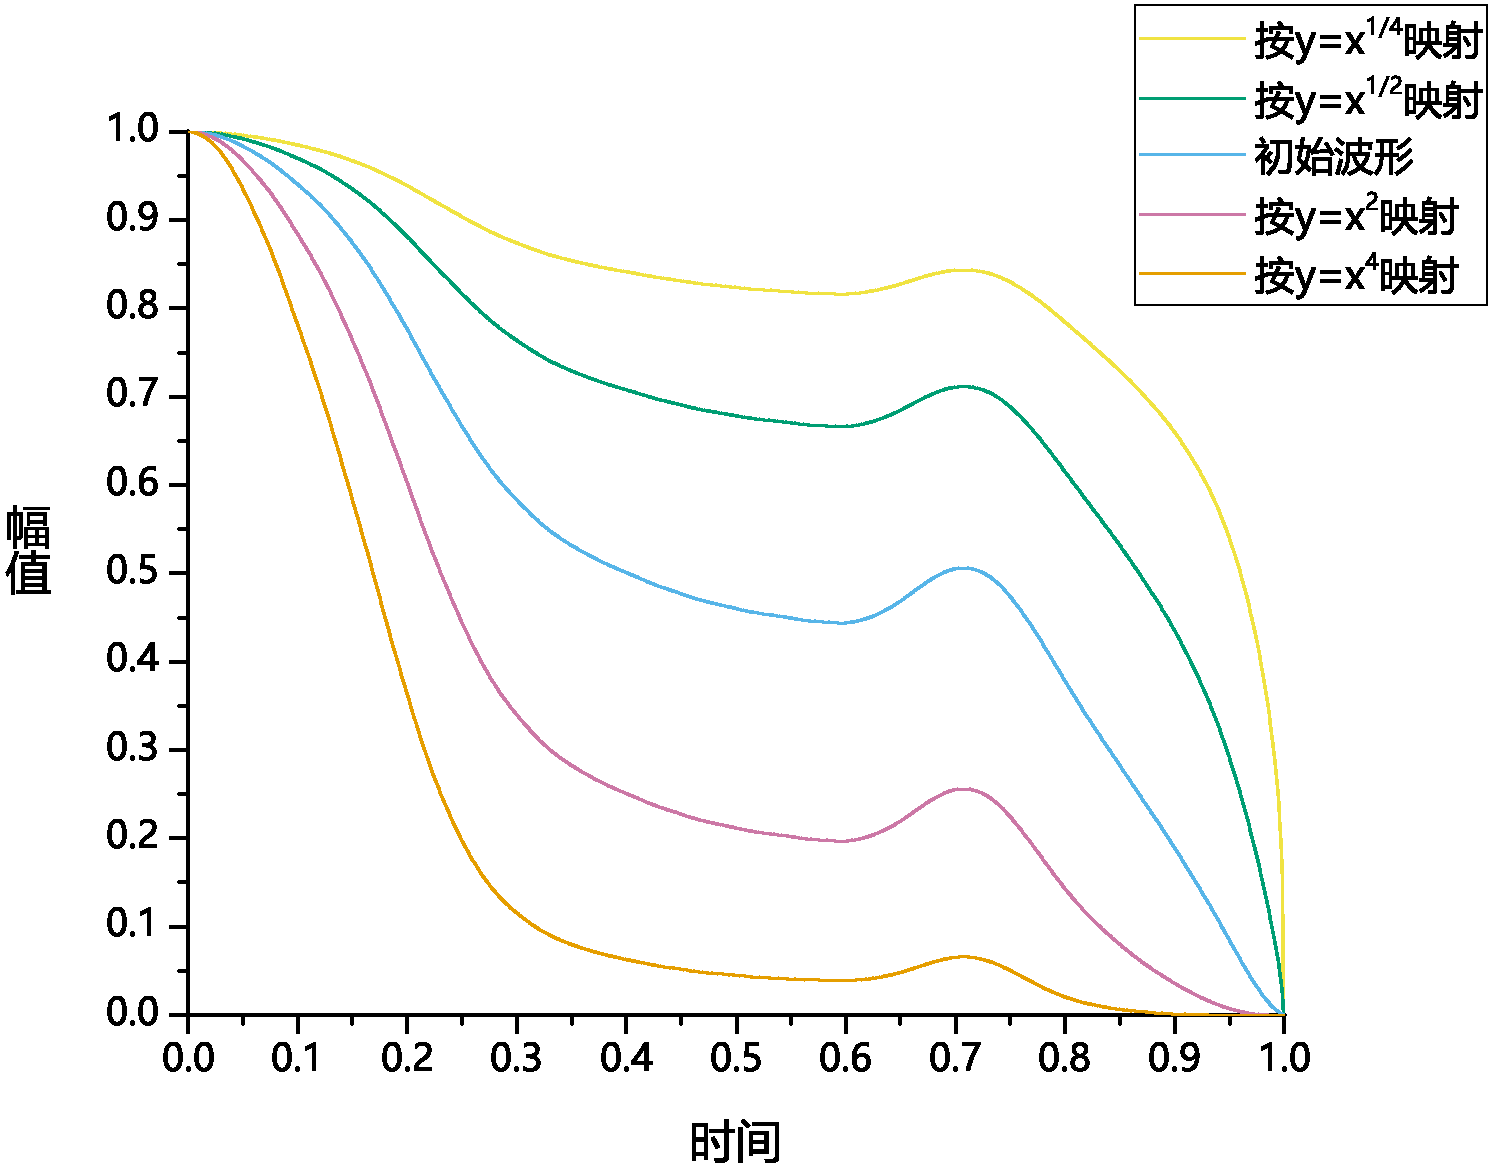
\includegraphics[width=5.5cm]{pulse_preprocess/edi1}
    }
    \quad
    \subfigure[\label{fig:edi2}对\autoref{fig:pulsecontrast}中脉搏波波形进行EDI计算 II]{
    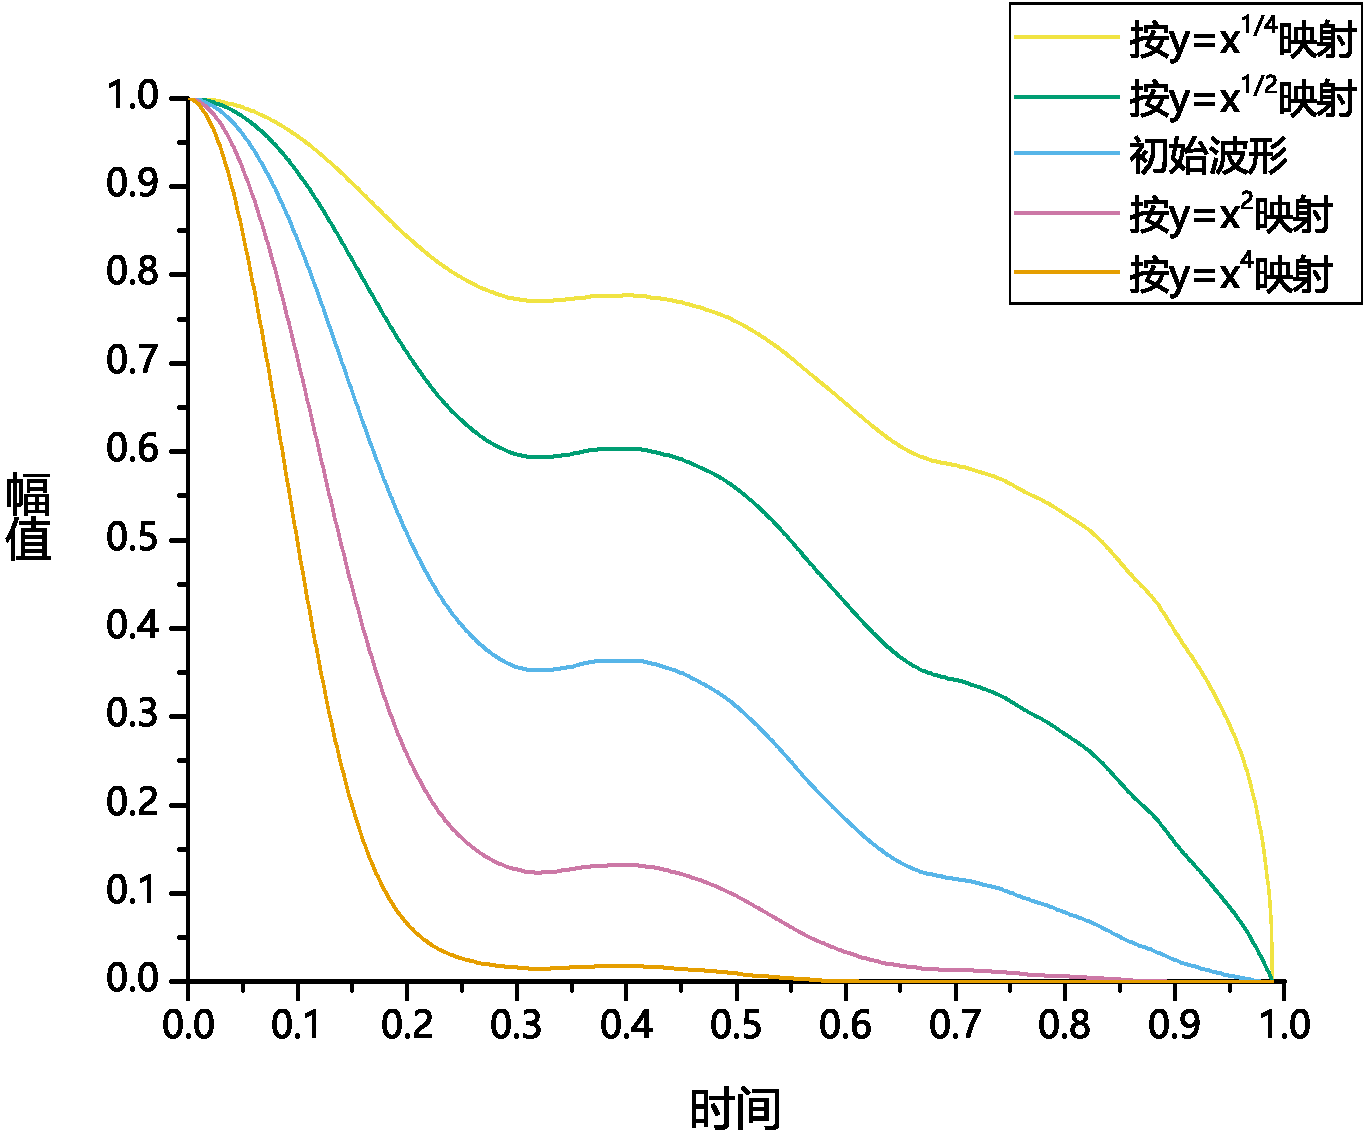
\includegraphics[width=5.5cm]{pulse_preprocess/edi2}
    }
    \quad
    \subfigure[\label{fig:edi3}对\autoref{fig:pulsecontrast}中脉搏波波形进行EDI计算 III]{
    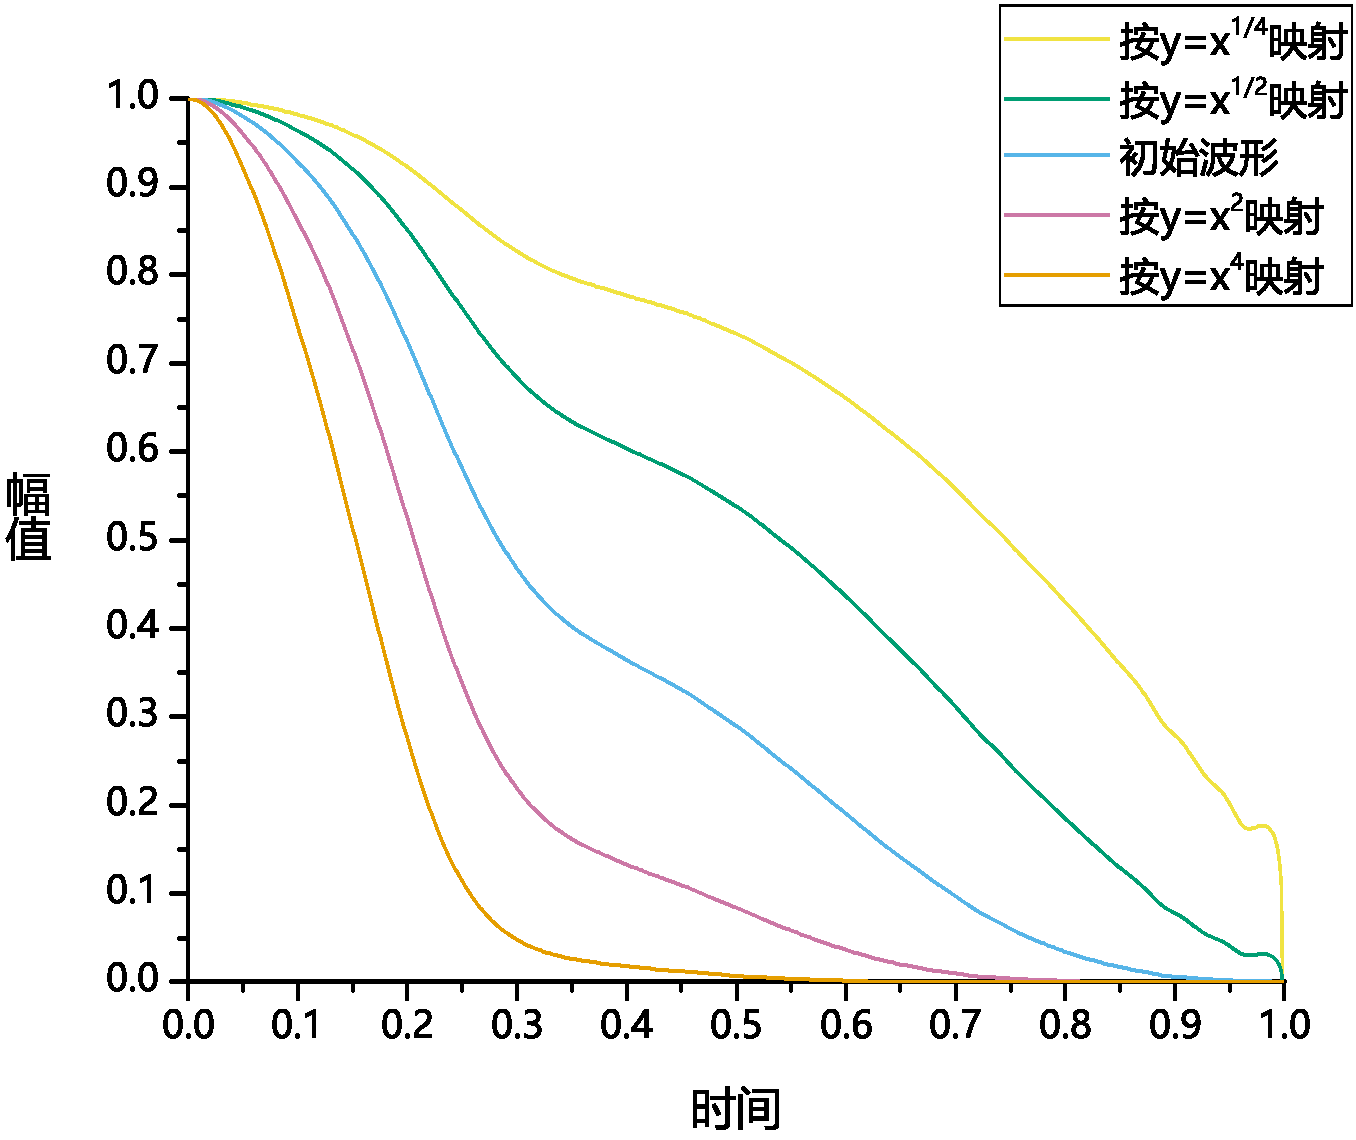
\includegraphics[width=5.5cm]{pulse_preprocess/edi3}
    }
    \caption{\label{fig:powandedi}幂函数簇与PPG波形的EDI指标示意}
\end{figure}

为解决上述问题,本研究首创提出了膨胀-腐蚀面积指数(erode and dilate area index,EDAI)这一新的描述方法。如\autoref{fig:powandedi}所示,EDAI的基本思路是利用幂函数簇的相关性质,
对\autoref{equ:area1}的累加值进行一定的映射,先对原始波形数据进行一次非线性变换
\begin{equation}
    \label{equ:area3}
    S \approx \frac{\Delta t}{2} \sum_{i=0}^{n-1}{(\boldsymbol F (P(i))+\boldsymbol F (P(i+1)))}
\end{equation}
其中,$\boldsymbol F$是幂指数函数簇。若将波形数据经幂函数$\boldsymbol F(x)=x^n$映射后的图形面积记为$S_n$,
那么,EDAI可以记为
\begin{equation}
    \label{equ:edai}
    EDAI_{k}=[S_{n_1},S_{n_2},\cdots,S_{n_k}]
\end{equation}
其中,$S_{n_k} \neq 0$。对比\autoref{equ:featurevector}可以发现,EDAI也是本研究先前定义的脉搏波波形特征描述向量的一个具体实例。

由相关数学知识可知,幂函数$\boldsymbol F(x)=x^n$在其定义域内均保持单调递增的性质。特别地,若限定函数定义域$x\subseteq [0,1]$,对于$n>1$的幂指数函数,$f(x)$均在$y=x$图像的下方,且$n$值越大,图像越贴近$x$轴,
函数图像“腐蚀”得越发严重;反之,$0<n<1$的幂指数函数会使$y=x$的图像趋近于直线$x=1$,$n$值越大,函数图像“膨胀”得愈益明显,如图\autoref{fig:pow}所示。
此时,若选取某一具体的幂函数,对所有采样点数值进行映射处理,相当于对原始波形图像进行了一次非线性拉伸变换。而幂函数本身的单调性可以保证这样的非线性缩放结果也是唯一的,
如图\autoref{fig:edi1}-图\autoref{fig:edi3}所示。若同时使用多个不同的幂函数进行上述处理,PPG波形上的差异必然在体现其对应的映射数值上,最终的面积累积值必然有所差异,
从而在面积类参数中保留了PPG波形细节信息。

\subsection{脉搏波波形间的描述}
在某些情景下,相较脉搏波间的共性特征而言,PPG波形间的差异(或者称之为PPG波形的紊乱程度)可能更需要被研究者们关注,如\autoref{fig:diff_in_pulse}所示。
如何评估、量化这种波形间乃至整条数据中所有波形之间的差异是本小节要阐述的重点。
\begin{figure}[htbp]
    \centering
    \subfigure[\label{dp0}正常孕妇的波形]{
    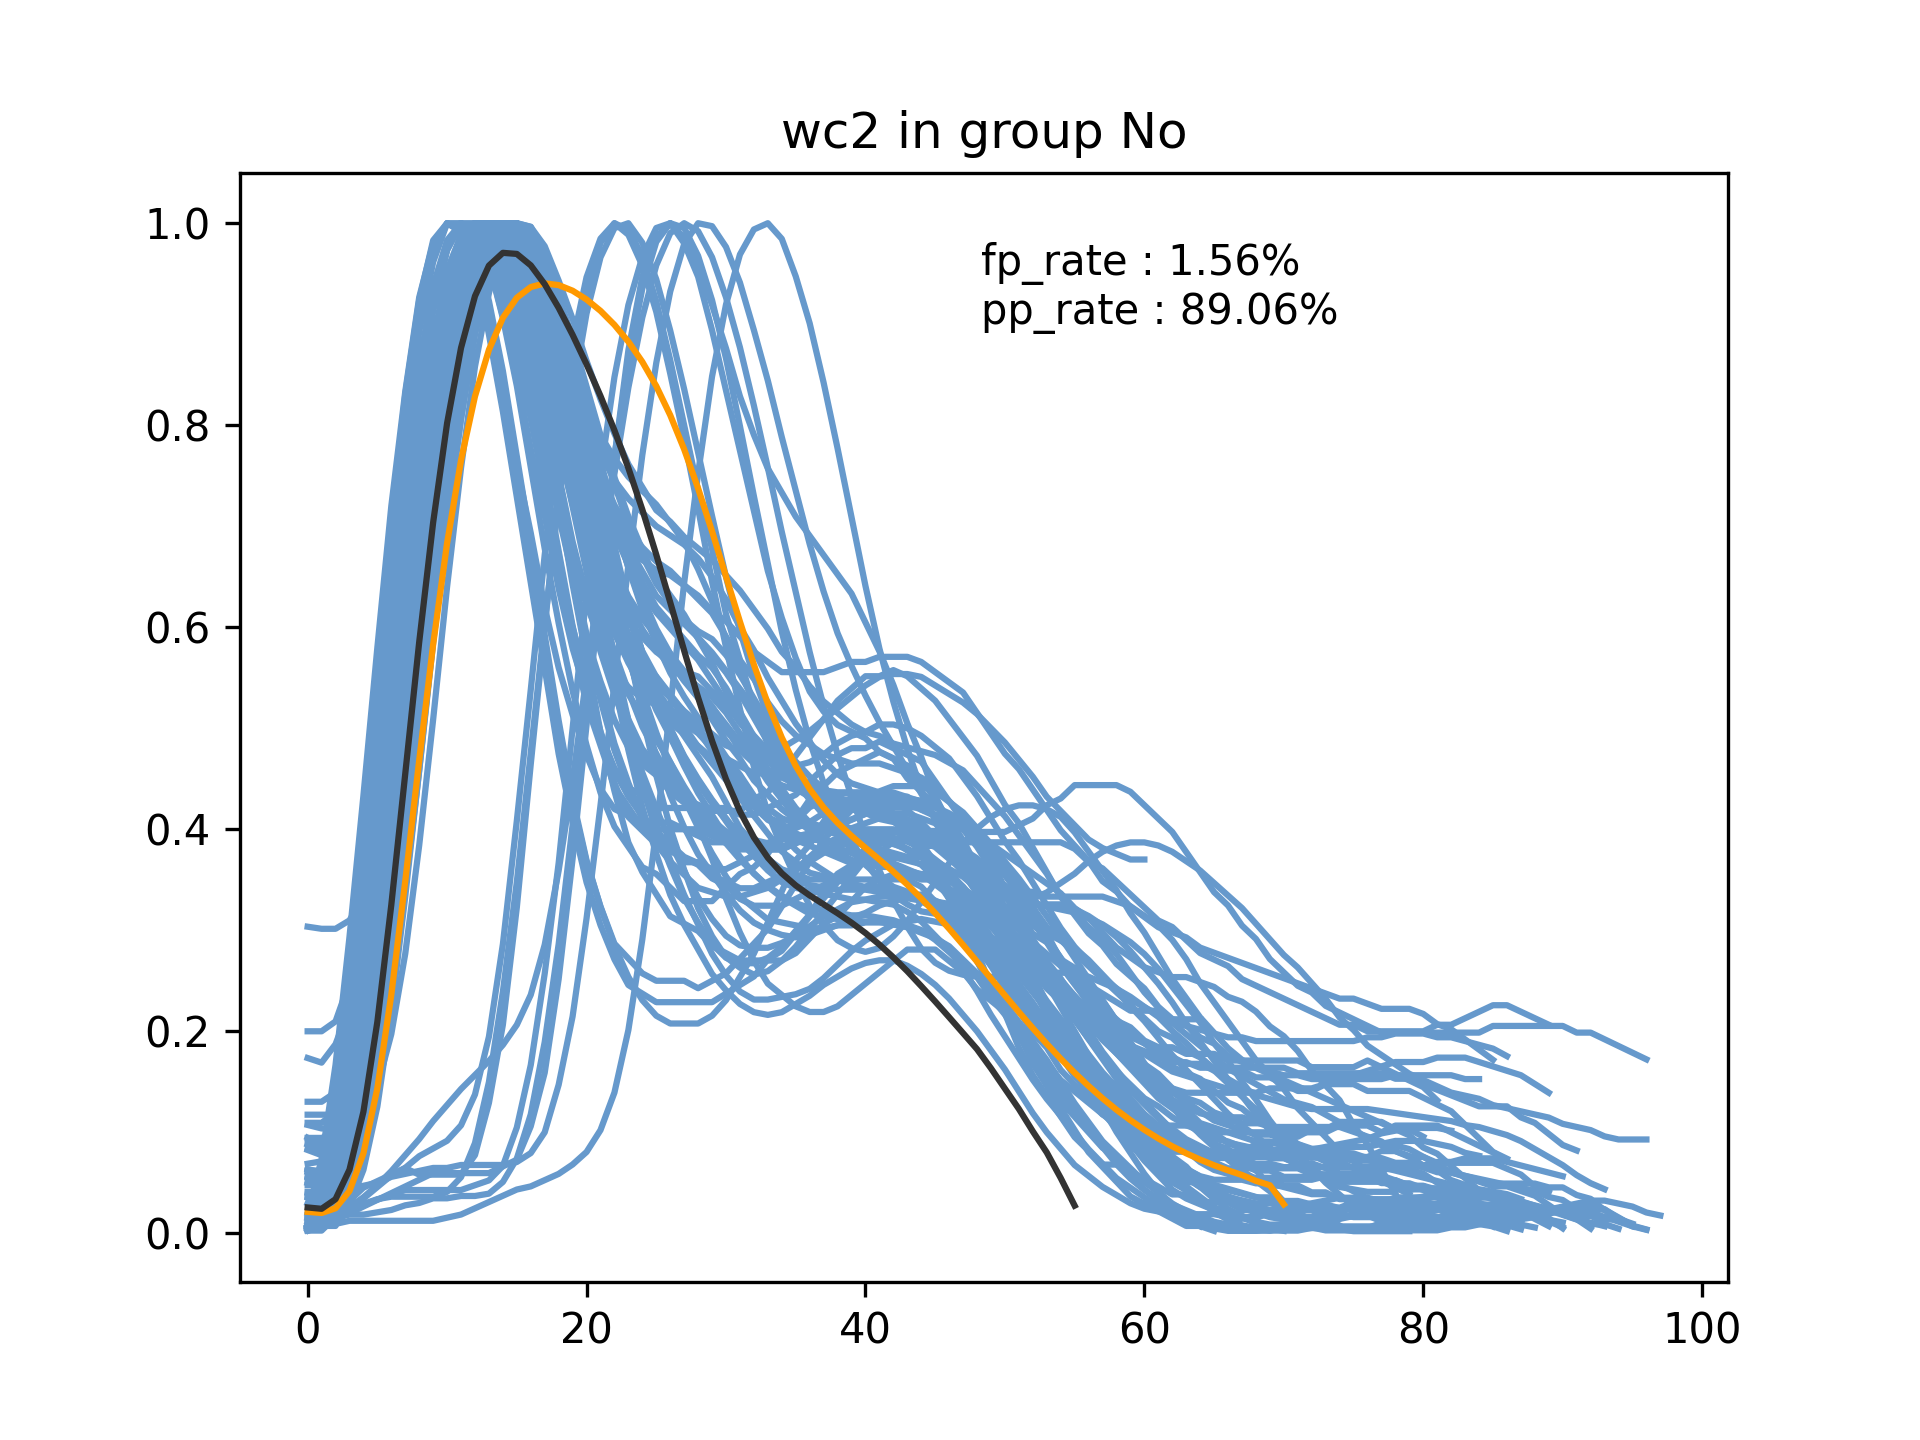
\includegraphics[width=6cm]{pulse_preprocess/wc2 in group No}
    }
    \quad
    \subfigure[\label{fig:dp1}患有PE孕妇的波形]{
    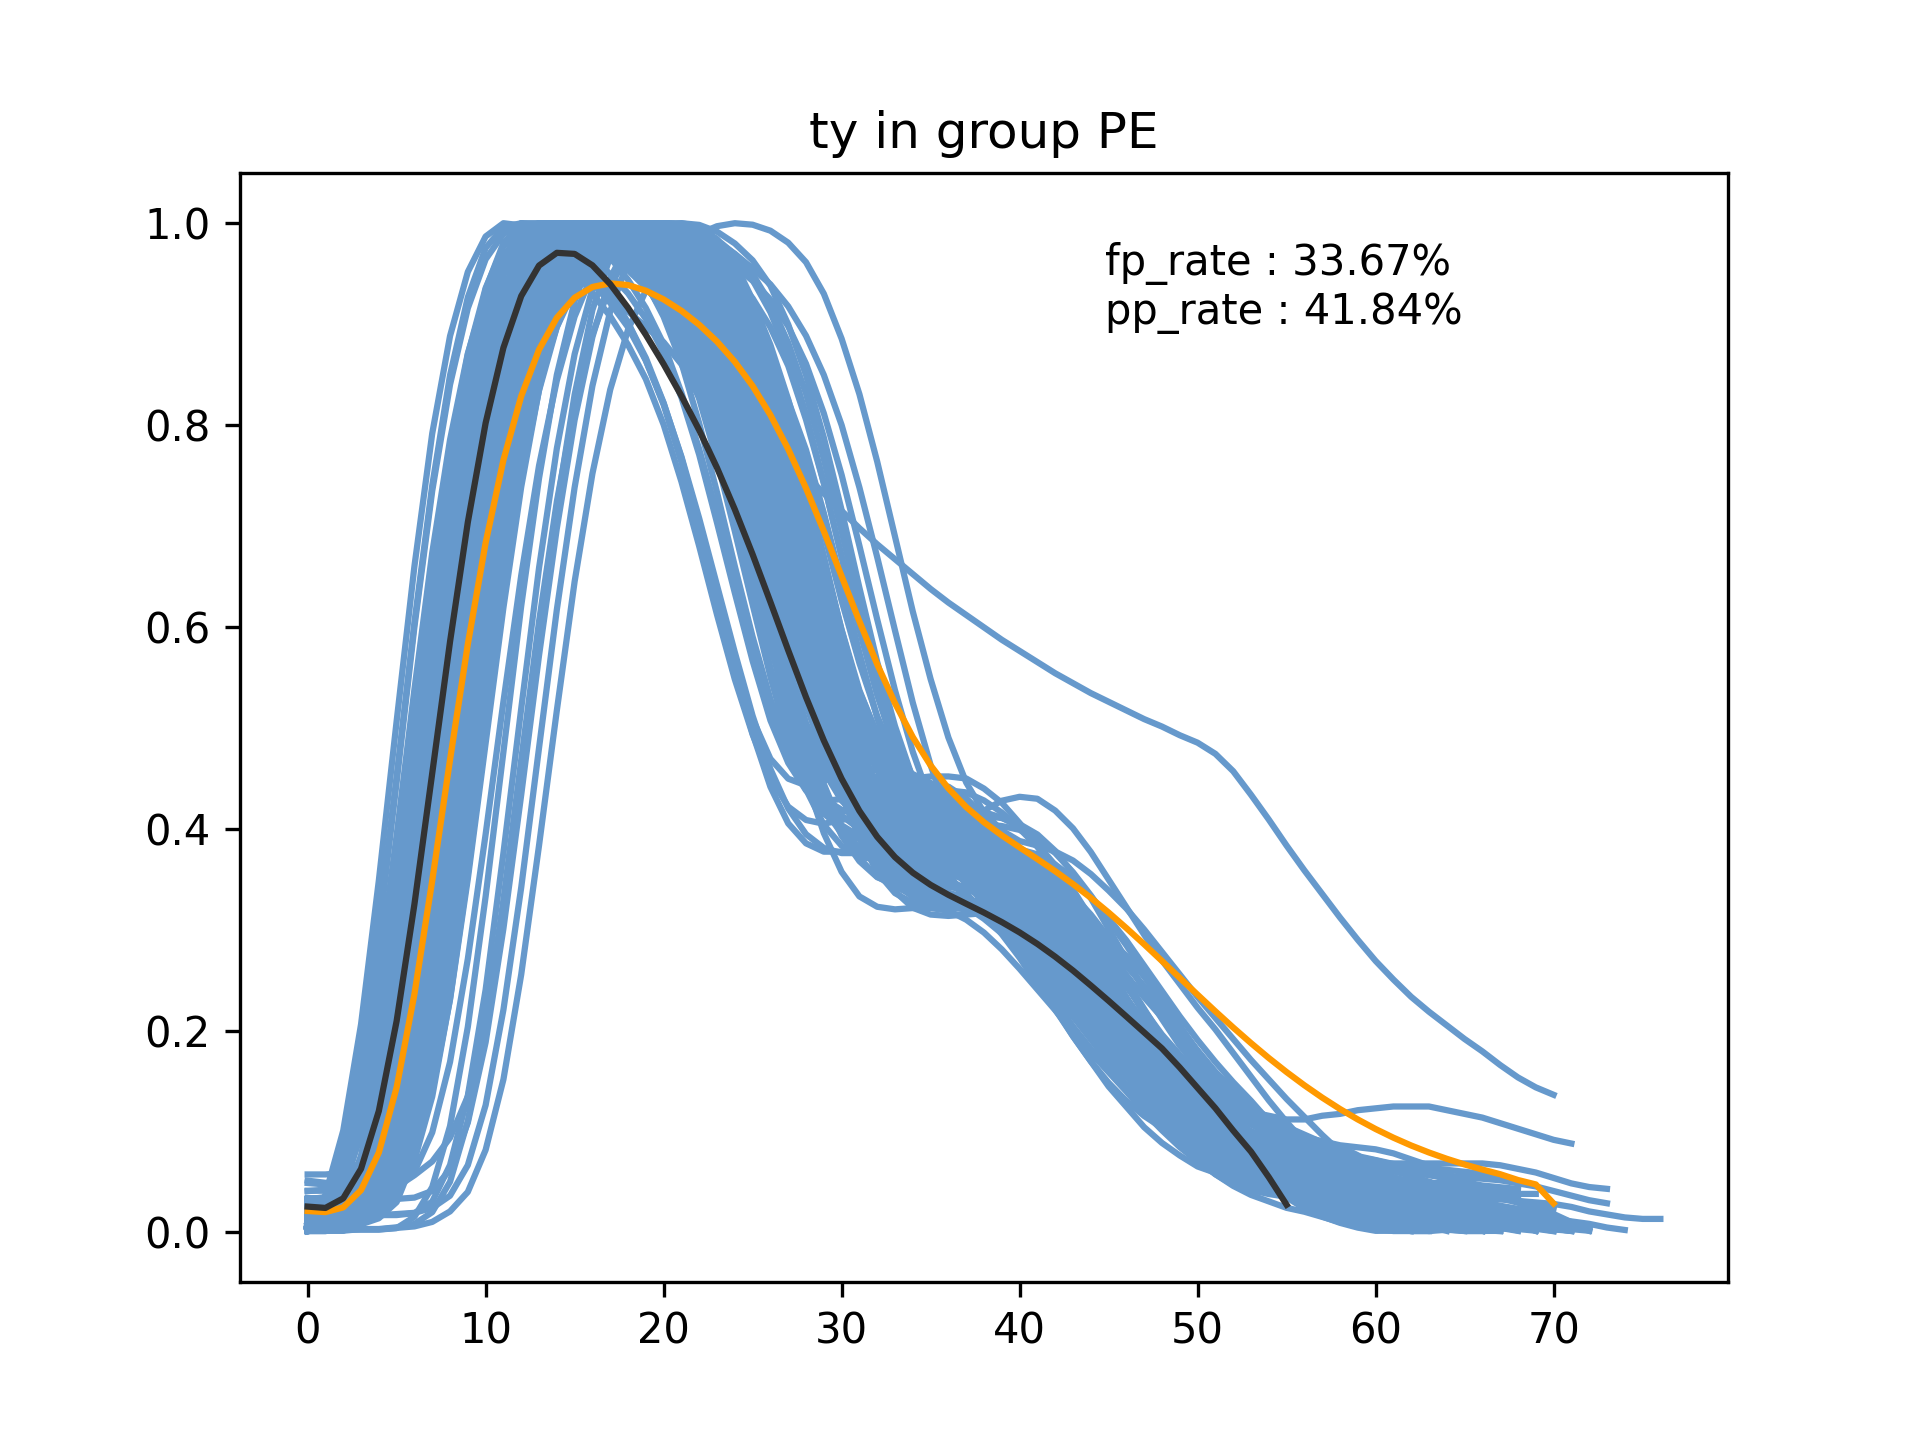
\includegraphics[width=6cm]{pulse_preprocess/ty in group PE}
    }
    \caption[脉搏波波形间的差异性]{\label{fig:diff_in_pulse}脉搏波波形间的差异性。使用了本研究自行采集的数据,所有波形经标准化后按起点进行了对齐。}
\end{figure}

本章此前介绍的PPG各项特征参数的设计逻辑多数是以一个完整波形为基本单位并对其进行量化描述,若直接用这些参数描述波形间的差异,会存在描述不够直接与描述能力有局限性等两项不足。
其中,前者是指波形间的差异能在具体参数的数值上得到体现,但差异的具体程度有待商榷;后者是指若出现涉及多个波形间的差异比较的情景,之前的参数会更显乏力。
鉴于此,本研究特进行了以下探索性研究。

一、两个波形的差异描述

本研究提出了互相关系数、Frechet距离及包络面积等三种参数量化描述脉搏波波形间的差异性。
此外,还对这三种参数的最容易遇到的对齐问题给出了一种可行解决思路。

1. 描述参数

\Rnum{1}. 相关系数

本文的第二章已经介绍过相关系数的这一变量分析方法,如\autoref{fig:relation}所示。由于相关系数本身就是作为衡量两个变量因素的密切程度而设计的,
因此,一种可行的办法是直接用相关系数去衡量两个波形之间的“相似”程度。需要注意的是,斯皮尔曼相关系数在计算时要求必须原始数据进行排序操作,而这一操作无疑会直接破坏波形的数据信息。
故本文最终选取了皮尔逊相关系数$r_p$进行表征
\begin{equation}
    \label{equ:pearson2}
    r_p=\frac{\sum_{i=1}^n{(x_i- \mathop{x} \limits^-)(y_i- \mathop{y} \limits^-)}}{\sqrt{{\sum_{i=1}^n}{{(x_i- \mathop{x} \limits^-)^2\sum_{i=1}^n}{(y_i- \mathop{y} \limits^-)^2}}}}
\end{equation}
波形间相关系数值越大,两者越“相似”。

\Rnum{2}. 弗朗明歇距离

弗朗明歇距离(Fréchet distance,FD)是最早由法国数学家Maurice René Fréchet于1906年提出的一种路径空间相似形描述方法\cite{Wien1994,Kaveh2013,GN2017}。
\autoref{fig:frechet distance}给出了FD定义的示意图。一种最经典、形象的理解是人牵着一条狗沿着不同的轨迹行走,两者之间最大的最短距离就是狗绳长度的下限,
这个值即为弗朗明歇距离。
\begin{figure}[htbp]
    \centering
    \subfigure[\label{fd0}弗朗明歇距离的形象示意]{
    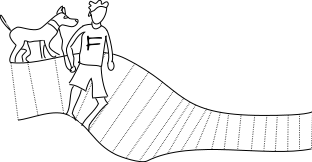
\includegraphics[width=6cm]{pulse_preprocess/frechet_distance0}
    }
    \quad
    \subfigure[\label{fig:fd1}弗朗明歇距离的数学示意\cite{GN2017}]{
    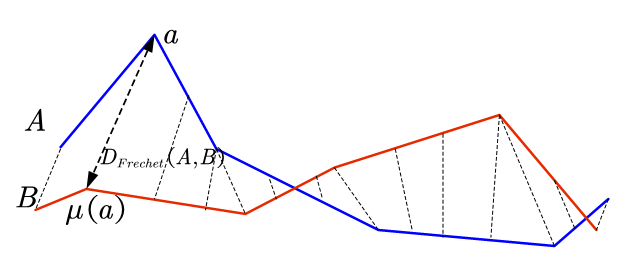
\includegraphics[width=6cm]{pulse_preprocess/frechet_distance1}
    }
    \caption{\label{fig:frechet distance}弗朗明歇距离的定义}
\end{figure}

FD的完整数学定义如下,若将曲线视为其在定义域至度量空间的一种映射关系,即$[a,b]\rightarrow V$,
那么对曲线$f:[a,b]\rightarrow V$与曲线$g:[a',b']\rightarrow V$,两者的弗朗明歇距离为
\begin{equation}
    \label{equ:frechet distance}
    \delta_F(f,g)=\inf \max \limits_{\alpha,\beta \; t \in (0,1)} d(f(\alpha(t)), g(\beta(t)))
\end{equation}
其中,$\alpha$与$\beta$是满足能将$[0,1]$分别映射至$[a,b]$与$[a',b']$的任意连续非递减函数,$d$是$V$上的度量函数\cite{Wien1994}。
一般而言,弗朗明歇距离的计算是个递归过程。
波形间的弗朗明歇距离值越小,两者越“相似”。

\Rnum{3}. 包络面积差

包络面积差(difference of envelope area ,DEA)是本研究提出的用以描述脉搏波间差异的原创指标。如\autoref{fig:dea}所示,其计算原理是计算两个经幅值归一化后的波形的按起点对齐后,由这两个波形围起来的区域的累计面积
\begin{equation}
    \label{equ:dea}
    \begin{aligned}
        S &= \int_{t_0}^{t_n}|P_f(t)-P_g(t)|dt\\
        &\approx \frac{\Delta t}{2} \sum_{i=0}^{n-1}{|(P_f(i)+P_f(i+1)-(P_g(i)+P_g(i+1))|}
    \end{aligned}
\end{equation}
\begin{figure}[htbp]
    \centering
    \subfigure[\label{fig:dea0}原始采样的包络面积差示意]{
    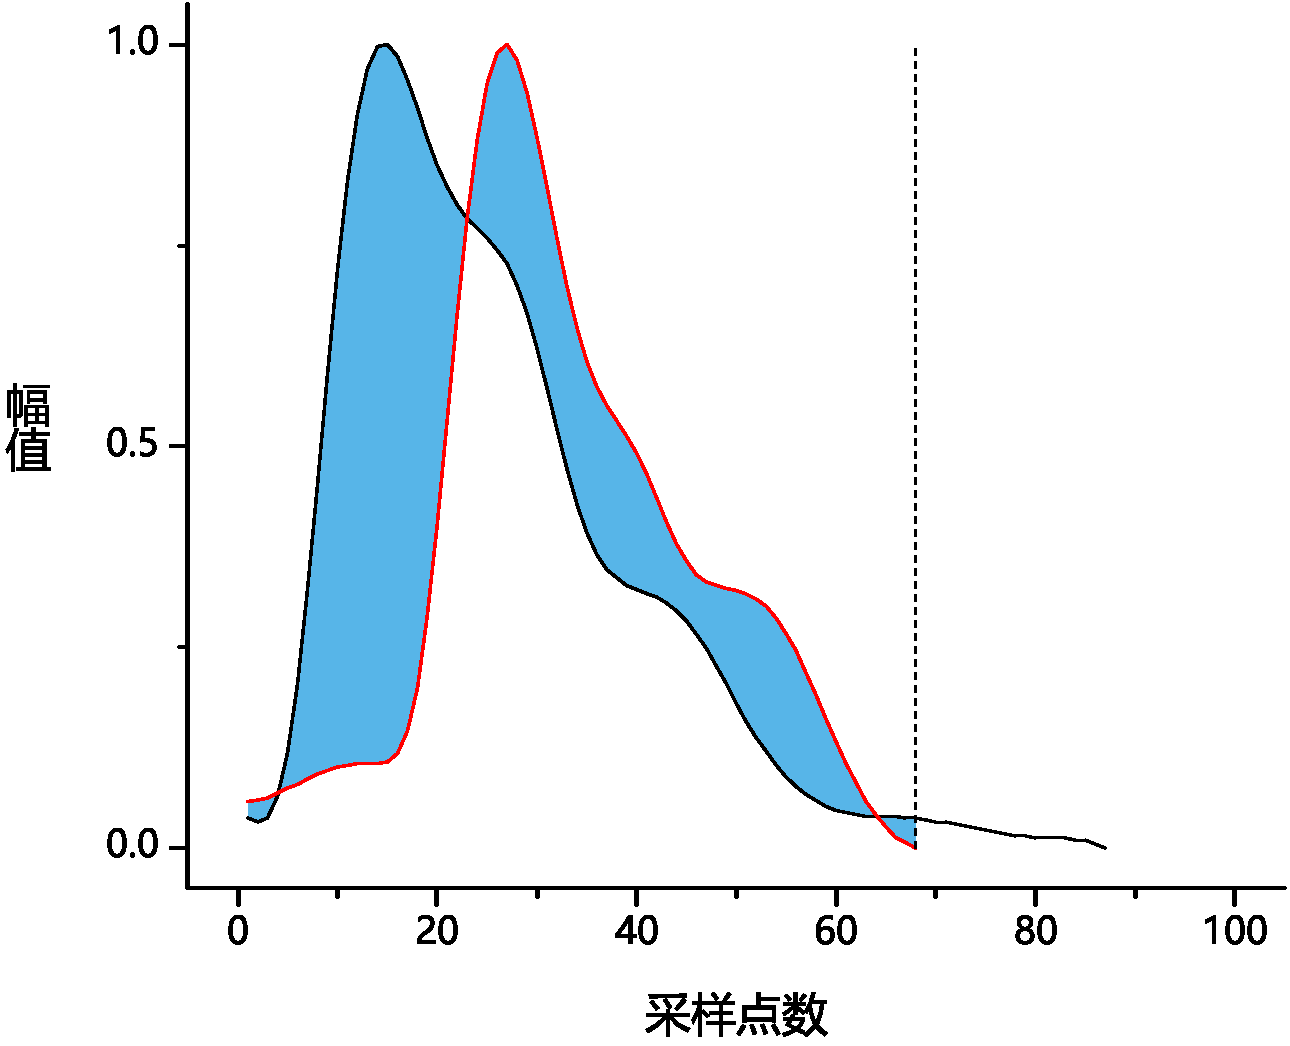
\includegraphics[width=6cm]{pulse_preprocess/dea0}
    }
    \quad
    \subfigure[\label{fig:dea1}重采样后的包络面积差示意]{
    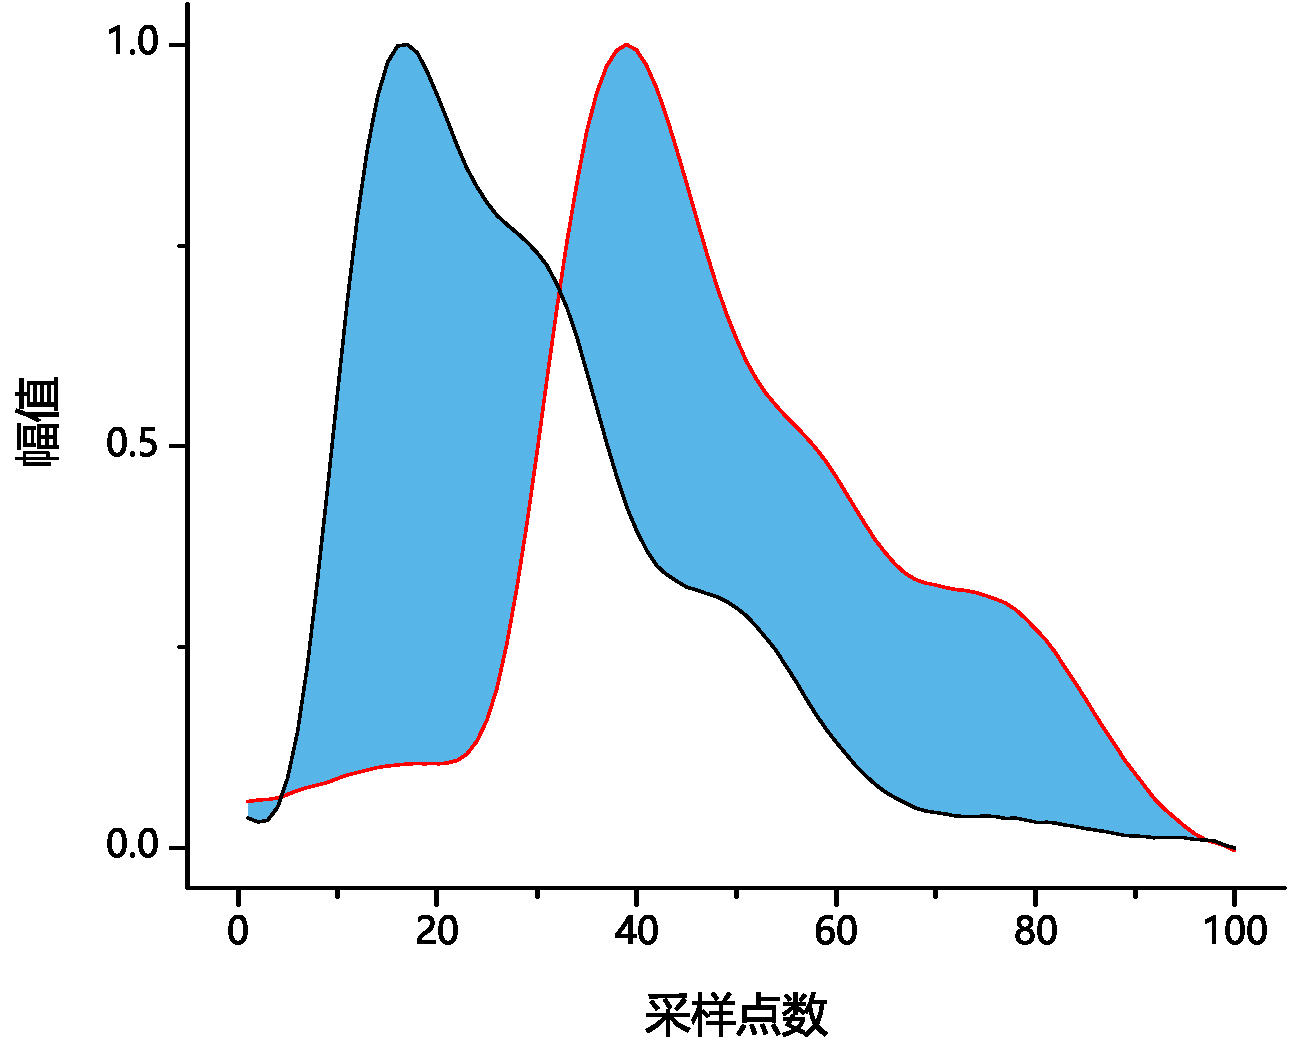
\includegraphics[width=6cm]{pulse_preprocess/dea1}
    }
    \caption[包络面积差示意]{\label{fig:dea}包络面积差示意。注意左图中虚线之后的数据处理。}
\end{figure}
波形间包络面积差值越小,两者越“相似”。

2. 波形采样点对齐

上述三个描述参数的计算过程都包含了一个隐藏的前置条件,即参与计算的两个波形的时间序列有着相等的采样点数。但如\autoref{fig:diff_in_pulse}与\autoref{fig:dea}所示,
由于脉搏波信号本身的随机性,这样的条件在实际中几乎不可能被满足。这也要求我们在计算这些参数时必须考虑波形的采样点数对齐问题。若将参与比较的两个波形的采样点数
分别记为$m$、$n$且$m \neq n$,不失一般性,设$m>n$,那么可行的解决思路有以下三种:

\Rnum{1}. 长端截取

此思路是只对两波形的前n个采样点进行计算,较长波形剩余$m-n$个采样点不参与计算。

\Rnum{2}. 短端补值

此思路是对较段波形在末端进行补值处理使其采样点数也为$m$,新增的补值可以设为0。

\Rnum{3}. 重采样至相同数值

与上述的截取、补值处理不同,重采样的处理逻辑是将两个波形的采样点数调整至相同。如在本章信号预处理小节中介绍的,通过信号的插值与抽取即可调整数据采样率。
若需将采样长度为$m$的波形调整至$k$,记$m$与$k$的最小公倍数为$p$,此时只需将原始数据均匀插值至$p$点,再按每$p/k$个点进行抽取即可。重采样前后的波形对比如\autoref{fig:dea}所示。

最后,需要指出的是,弗朗明歇距离的计算过程是一个递归过程,目前很多具体的实现算法均已可以对长度不对齐的两个序列进行计算\cite{derohde2022}。

二、更多波形间的差异性描述

前文介绍的是对两个波形间的差异的描述,对更多的波形间的描述也可按照这种思路进行。具体而言,若需量化\autoref{fig:diff_in_pulse}所示n个波形间的整体差异性,可按排列组合的方法每次从n个波形间
选取两个波形,并用上述三种描述参数进行量化,最终会得到3组数据,每组有$C_n^2$个具体数值。此时,可按数理统计的一般方法,用这3组数据的平均值、方差、标准差、极值等指标进行这n个
波形的整体性描述。

\section{小结}
本章主要对脉搏波信号的预处理过程与参数描述进行了详细的说明。针对脉搏波预处理,本章对信号滤波、波型检测、重博波检测、基线漂移去除、插值及标准化过程进行了介绍,并重点解释
了本研究提出的一种新型模块化脉搏波波形检测算法,即初筛-复核-投票算法。该算法具有检测准确度高、抗干扰能力强、可拓展性强等优点。
针对脉搏波的参数描述,本章首先从方法论的角度概括了参数描述的意义与本质,随后从常见的脉搏波时域描述参数及本研究原创提出的描述参数对研究内容进行了介绍。
其中,原创提出的脉搏波描述参数包含描述脉搏波波形及波形之间差异性等两大类。
本章的相关研究内容为后续章节所进行数据分析工作打下了坚实的基础。